%%%%%%%%%%%%%%%%%%%%%%%%%%%%%%%%%%%%%%%%%%%%%%%%%%%%%%%%%%%%%%%%%%%%%%%%%%%%%%%%%%%%%%%%%%%%%%%%%%%%%
% This template is distributed with ABSOLUTELY NO WARRANTY.
% It serves as a guideline and constitutes a basic structure for a
% thesis/dissertation. The user assumes full responsibility for formatting
% and typesetting their document and for verifying that all the thesis
% requirements set by the University of Tennessee are met. Please refer to the most
% recent UT thesis guide (http://web.utk.edu/~thesis/thesisresources.shtml)
% or contact the thesis consultant (http://web.utk.edu/~thesis/).
% Please report any bugs to the thesis consultant.
%%%%%%%%%%%%%%%%%%%%%%%%%%%%%%%%%%%%%%%%%%%%%%%%%%%%%%%%%%%%%%%%%%%%%%%%%%%%%%%%%%%%%%%%%%%%%%%%%%%%%
% O P T I O N S:
% 1. thesis/dissertation
% 2. monochrome
% 3. all options provided by the report class
\documentclass[thesis,letterpaper,12pt]{utthesis} % thesis, one side
% some alternatives are:
%\documentclass[thesis,monochrome,letterpaper,12pt]{utthesis} %thesis, one side, monochrome text
%\documentclass[thesis,twoside,letterpaper,12pt]{utthesis} % thesis, two side
%\documentclass[thesis,monochrome,twoside,letterpaper,12pt]{utthesis} % thesis, two side, monochrome text
% for a dissertation, replace the thesis option by dissertation:
% \documentclass[dissertation,letterpaper,12pt]{utthesis} . . .
\renewcommand{\baselinestretch}{1.5} 	 % line Spacing
%%%%%%%%%%%%%%%%%%%%%%%%%%%%%%%%%%%%%%%%%%%%%%%%%%%%%%%%%%%%%%%%%%%%%%%%%%%%%%%%%%%%%%%%%%%%%%%%%%%%%
% TO DO: FILL IN YOUR INFORMATION BELOW - READ THIS SECTION CAREFULLY
%%%%%%%%%%%%%%%%%%%%%%%%%%%%%%%%%%%%%%%%%%%%%%%%%%%%%%%%%%%%%%%%%%%%%%%%%%%%%%%%%%%%%%%%%%%%%%%%%%%%%
\title{Hot Ductility Behavior of 20Cr-32Ni-1Nb Heat-Resistant Stainless Steel}	       % title of thesis/dissertation
\author{John William Bohling}                % author's name
\copyrightYear{2016}            % copyright year of your thesis/dissertation
\graduationMonth{August}           % month of graduation of your thesis/dissertation
\majorProfessor{Carl D. Lundin}	    % advisor's name
\keywords{Hot ductility, Gleeble, 20Cr-32Ni-1Nb, Stainless steel}	% keywords (optional) separated by commas - these are used in the PDF file properties
\viceProvost{Dixie Thompson} % vice provost name
\major{Materials Science and Engineering}	% major: Mechanical Engineering, Aerospace Engineering, Mathematics...
\degree{Master of Science}	    % degree: Doctor of Philosophy, Master of Science, Master of Engineering...
\college{Engineering}           % college
\dept{Materials Science and Engineering}	% department
\university{The University  of Tennessee, Knoxville}	% school name
% THIS TEMPLATE ACCOMMODATES UP TO 5 COMMITTEE MEMBERS - ENTER ONLY THE NAMES OF THE MEMBERS ON YOUR COMMITTEE
\numberOfCommitteeMembers{2} % enter the number of committee members
\committeeMemberA {Hahn Choo}	% name of first committee member
\committeeMemberB {Carl J. McHargue}	% name of second committee member
\committeeMemberC {Committee Member 3}	% ... you get the trend!
\committeeMemberD {Committee Member 4}	% if your committee has less than 4 members, you do not need to edit the
\committeeMemberE {Committee Member 5}  % rest of committee names
%%%%%%%%%%%%%%%%%%%%%%%%%%%%%%%%%%%%%%%%%%%%%%%%%%%%%%%%%%%%%%%%%%%%%%%%%%%%%%%%%%%%%%%%%%%%%%%%%%%%%
% LOAD SOME USEFUL PACKAGES
%%%%%%%%%%%%%%%%%%%%%%%%%%%%%%%%%%%%%%%%%%%%%%%%%%%%%%%%%%%%%%%%%%%%%%%%%%%%%%%%%%%%%%%%%%%%%%%%%%%%%
\usepackage{lmodern}
\usepackage{nomencl}                    % produces a nomenclature
\usepackage{float}                      % figure floats
%\usepackage[square,numbers]{natbib}                     % this package allows you to link your references

%\usepackage[pagebackref=true]{hyperref}

\usepackage{csquotes}
\usepackage[english]{babel}
\usepackage[natbib=true,style=ieee,backref=true,hyperref=true,backend=biber]{biblatex}
\addbibresource{references/references-thesis.bib}
\usepackage{graphicx}					% graphics package
\graphicspath{ {figures/}{figures/eps/}{figures/pdf/} }% specify the path where figures are located
\usepackage{fancyhdr}                   % fancy headers and footers
\usepackage{url}                        % nicely format url breaks
\usepackage[inactive]{srcltx}		 	% necessary to use forward and inverse searching in DVI
\usepackage{relsize}                    % font sizing hierarchy
\usepackage{booktabs}                   % professional looking tables
\usepackage[config, labelfont={bf}]{caption,subfig} % nice sub figures
\usepackage{mathrsfs}                   % additional math scripts
\usepackage{flafter}                    % force floats to be placed after their definition
%%% PACKAGES THAT ARE PRELOADED WITH THE CLASS ARE: amsmath,amsthm,amssymb,setspace,geometry,hyperref,and color
%%%%%%%%%%%%%%%%%%%%%%%%%%%%%%%%%%%%%%%%%%%%%%%%%%%%%%%%%%%%%%%%%%%%%%%%%%%%%%%%%%%%%%%%%%%%%%%%%%%%%
\begin{document}
    \pagenumbering{alph} % this is needed to clear certain issues with the hyperref package
    %
    \makeApprovalPage % make the approval page - this is the page that needs to be signed & returned to the thesis/dissertation consultant
    \makeETDApprovalPage % make the Electronic Thesis & Dissertation page - this page is kept with the electronic copy
    %
    \addToPDFBookmarks{0}{Front Matter}{rootNode} % create a root node named "Front Matter" in the pdf bookmarks
    \addToPDFBookmarks{1}{Title}{a} % add a pdf bookmark to the title page
    \makeTitlePage % make the title page. Make sure you properly set the \docType
    %
    \pagenumbering{roman}
    \setcounter{page}{2}
    %
    \makeCopyrightPage % make the copyright page
    %
    \addToPDFBookmarks{1}{Dedication}{b} % add a pdf bookmark to the dedication page
    \chapter*{}
\begin{center}
{\centering \it To my parents,
Mark and Sandra Bohling,
for their love and support in all my endeavours}
\end{center}  % include the dedication
    %
    \addToPDFBookmarks{1}{Acknowledgements}{c} % add a pdf bookmark to the acknowledgements page
    \chapter*{Acknowledgements}
I would like to thank the Materials Properties Council under the direction of Dr. Martin Prager and the Center for Materials Processing, directed by Dr. Claudia Rawn through the Department of Materials Science and Engineering at the University of Tennessee, Knoxville, for providing funding support for my work.  % include the acknowledgements
    %
    \addToPDFBookmarks{1}{Quote}{d} % add a pdf bookmark to the quotation page
    \chapter*{}
{\it Some quotation...} % include a quote
    %
    \addToPDFBookmarks{1}{Abstract}{e} % add a pdf bookmark to the abstract page
    \chapter*{Abstract}\label{ch:abstract}
Steam reforming of hydrocarbons is an important process for the production of hydrogen for industrial needs, such as ammonia synthesis. Due to the high temperature (\SIrange[range-phrase=--]{700}{900}{\degreeCelsius}) conditions, reformer furnace components require materials with excellent creep properties and thus highly alloyed austenitic stainless steels are typically employed. For reformer outlet manifolds, a cast, heat-resistant stainless steel with the composition 20Cr-32Ni-1Nb (ASTM A351 Grade CT15C) is widely used. However, after service exposure this alloy exhibits problems with liquation cracking in the base metal \gls{haz} during repair welding. In the work presented herein, two heats of material from centrifugally-cast manifold components were evaluated to quantify the potential susceptibility to \gls{haz} liquation cracking. The weldability of the 20Cr-32Ni-1Nb materials was evaluated using the Gleeble\texttrademark{} hot ductility test to determine the on-heating and on-cooling ductility (percent reduction in area) at various temperatures after exposure to a simulated welding thermal cycle. The as-received materials and selected hot ductility samples were characterized using \gls{olm} and \gls{sem} with \gls{eds} to correlate the hot ductility behavior with microstructural characteristics.

Both 20Cr-32Ni-1Nb heats showed similar hot ductility behavior when tested (\emph{i}) on-heating and (\emph{ii}) on-cooling from the measured \gls{zdt} of \SmartUnit{fahrenheit=2375}. The hot ductility curves revealed that both materials exhibited a poor recovery of on-cooling ductility (Class C3 based on the Nippes criteria) after exposure to the \gls{zdt}, with a noticeable \gls{zdr} and a low \gls{drr} on the order of 20\%. The microstructural evaluation revealed that the loss of on-heating and on-cooling ductility was a result of liquation along the interdendritic boundaries. \gls{eds} analysis did not reveal the presence of significant amounts of Ni-Nb-Si enriched phases adjacent to the niobium carbides. The observed liquation along the interdendritic boundaries was attributed to constitutional liquation of niobium carbides which were present in the boundary regions. Based on these findings, the two 20Cr-32Ni-1Nb heats are sensitive to \gls{haz} liquation cracking when exposed to a thermal cycle as would be encountered in repair welding.




%Repair welding of heat-resistant stainless steels used in steam reformer furnace components can be problematic if the material is in the service-exposed condition, due to liquation cracking in the base metal heat-affected zone (HAZ).  Service-exposed, cast 20Cr-32Ni-1Nb heat-resistant steel extracted from a reformer outlet manifold was evaluated using the Gleeble hot ductility test to determine its susceptibility to HAZ liquation cracking.  The hot ductility curves revealed that the service-exposed material exhibited poor ductility recovery when tested upon cooling from the on-heating zero ductility temperature (ZDT) of 2375°F.  On this basis, the service-exposed 20Cr-32Ni-1Nb material would be classified as fairly susceptible to HAZ liquation cracking when exposed to a welding thermal cycle. % your abstract
    %
    \addToPDFBookmarks{0}{Table of Contents}{f}
    \tableofcontents % generate a table of contents
    %
    \addToTOC{List of Tables} % this will add the list of tables to the Table of Contents (TOC)
    \listoftables % generate a list of tables
    %
    \addToTOC{List of Figures} % this will add the list of figures to the Table of Contents (TOC)
    \listoffigures % generate a list of figures
    %
    \makenomenclature % OPTIONAL
    \addToPDFBookmarks{0}{Nomenclature}{g} % OPTIONAL
    %\addToTOC{Nomenclature}
    \printnomenclature[1.25in] % OPTIONAL
    %
    \newpage
    \pagenumbering{arabic}
    \setcounter{page}{1}
    %%%%%%%%%%%%%%%%%%%%%%%%%%%%%%%%%%%%%%%%%%%%%%%%%%%%%%%%%%%%%%%%%%%%%%%%%%%%%%%%%%%%%%%%%%%%%%%%%%%%%
    % INCLUDE THE CHAPTERS STARTING WITH THE NOMENCLATURE IF PRESENT
    %%%%%%%%%%%%%%%%%%%%%%%%%%%%%%%%%%%%%%%%%%%%%%%%%%%%%%%%%%%%%%%%%%%%%%%%%%%%%%%%%%%%%%%%%%%%%%%%%%%%%
    %%!TEX root = ..\ms-thesis.tex
% enter the list of nomenclature here
\nomenclature{HAZ}{Heat-affected zone}
 % OPTIONAL
    %!TEX root = ..\ms-thesis.tex
\chapter{Introduction} \label{ch:introduction}

Steam reforming of hydrocarbons is an important industrial process for the production of hydrogen gas either as an end product or as an input for other processes such as ammonia synthesis and petroleum hydrocracking. In the steam reforming process, a hydrocarbon feedstock is reacted with steam, usually in the presence of a catalyst, to yield hydrogen gas and byproducts according to the following reactions \cite{rostrup-nielsen_catalytic_1984}:
\begin{align}
%\ce{C_{n}H_{m}}+\ce{n H2O} -> \ce{n CO}+\bigl(n+\frac{m}{2}\bigr)\ce {H2} \quad (-\Delta{}H^{0}_{298} < 0) \\
\ce{C_{n}H_{m} + n H2O -> n CO + } \bigl(n + \frac{m}{2}\bigr) \ce{H2} \quad (-\Delta{}H^{0}_{298} < 0) \label{eq:1} \\
\ce{CO + H2O <=> CO2 + H2} \quad (-\Delta{}H^{0}_{298} = 41.2 \, \text{kJ mol}^{-1}) \label{eq:2} \\
\ce{CO + 3H2 <=> CH4 + H2O} \quad (-\Delta{}H^{0}_{298} = 206.2 \, \text{kJ mol}^{-1}) \label{eq:3}
\end{align}
Most commonly, methane (CH$_{\textnormal{4}}$) in the form of natural gas is the preferred feedstock, although heavier hydrocarbons such as propane, naphtha, and heptane can be used depending upon availability and cost \cite{rostrup-nielsen_catalytic_1984,haussinger_hydrogen_2000}. In the above reactions, steam functions as an oxiziding agent to break apart the hydrocarbon; in some variants of the process, air is also added as a further oxidizer. The catalyst is typically nickel-based on an oxide substrate.

By adjusting the process conditions (exit temperature and amount of steam), the equilibria of the reforming reactions \ref{eq:1}--\ref{eq:3} can be modified to favor certain products and thereby adjust the composition of the product gas. For example, for ammonia synthesis which is one of the largest industrial consumers of hydrogen, the typical desired process conditions are 3.3 MPa exit pressure, 800C exit temperature, and a steam to carbon ratio of 3.7 \cite{rostrup-nielsen_catalytic_1984} to minimize the methane content in the product. Considering that reaction \ref{eq:1} is endothermic while reactions \ref{eq:2} and \ref{eq:3} are exothermic, under the process conditions just listed (for minimizing methane) the overall reaction is endothermic and thus external heating is required. The necessary heat is supplied by enclosing the reaction apparatus in a \emph{reformer furnace}.

An illustration of a typical reformer furnace is shown in Figure~\ref{fig:reformer-furnace}. The furnace is a tubular reformer design, in which the feedstock stream (e.g. containing natural gas and steam) is fed simultaneously through a series of identical tubes, containing the catalyst material, which are externally heated. These tubes are visible in Figure~\ref{fig:reformer-furnace} in a vertical arrangement, with the burners installed on the sides of the furnace walls. The inlet side where the preheated feedstock enters the tubes is at the top of the furnace, with the hot product gas mixture collected at an outlet manifold at the bottom of the furnace, consisting of ``hot side'' header, tee, and reducer ("cone") which connects to a refractory-walled transfer line. Through the transfer line, the product gas flow is directed to a waste heat recovery boiler which generates high-pressure steam to be used in the reformer \cite{rostrup-nielsen_catalytic_1984}. A photograph of another furnace is shown in Figure~\ref{fig:reformer-tee-cone} \cite{penso_repair_2006} in which the outlet pigtails (from the reformer tubes), the outlet header and tee, and cone are clearly visible.

\begin{figure}[h]
\centering
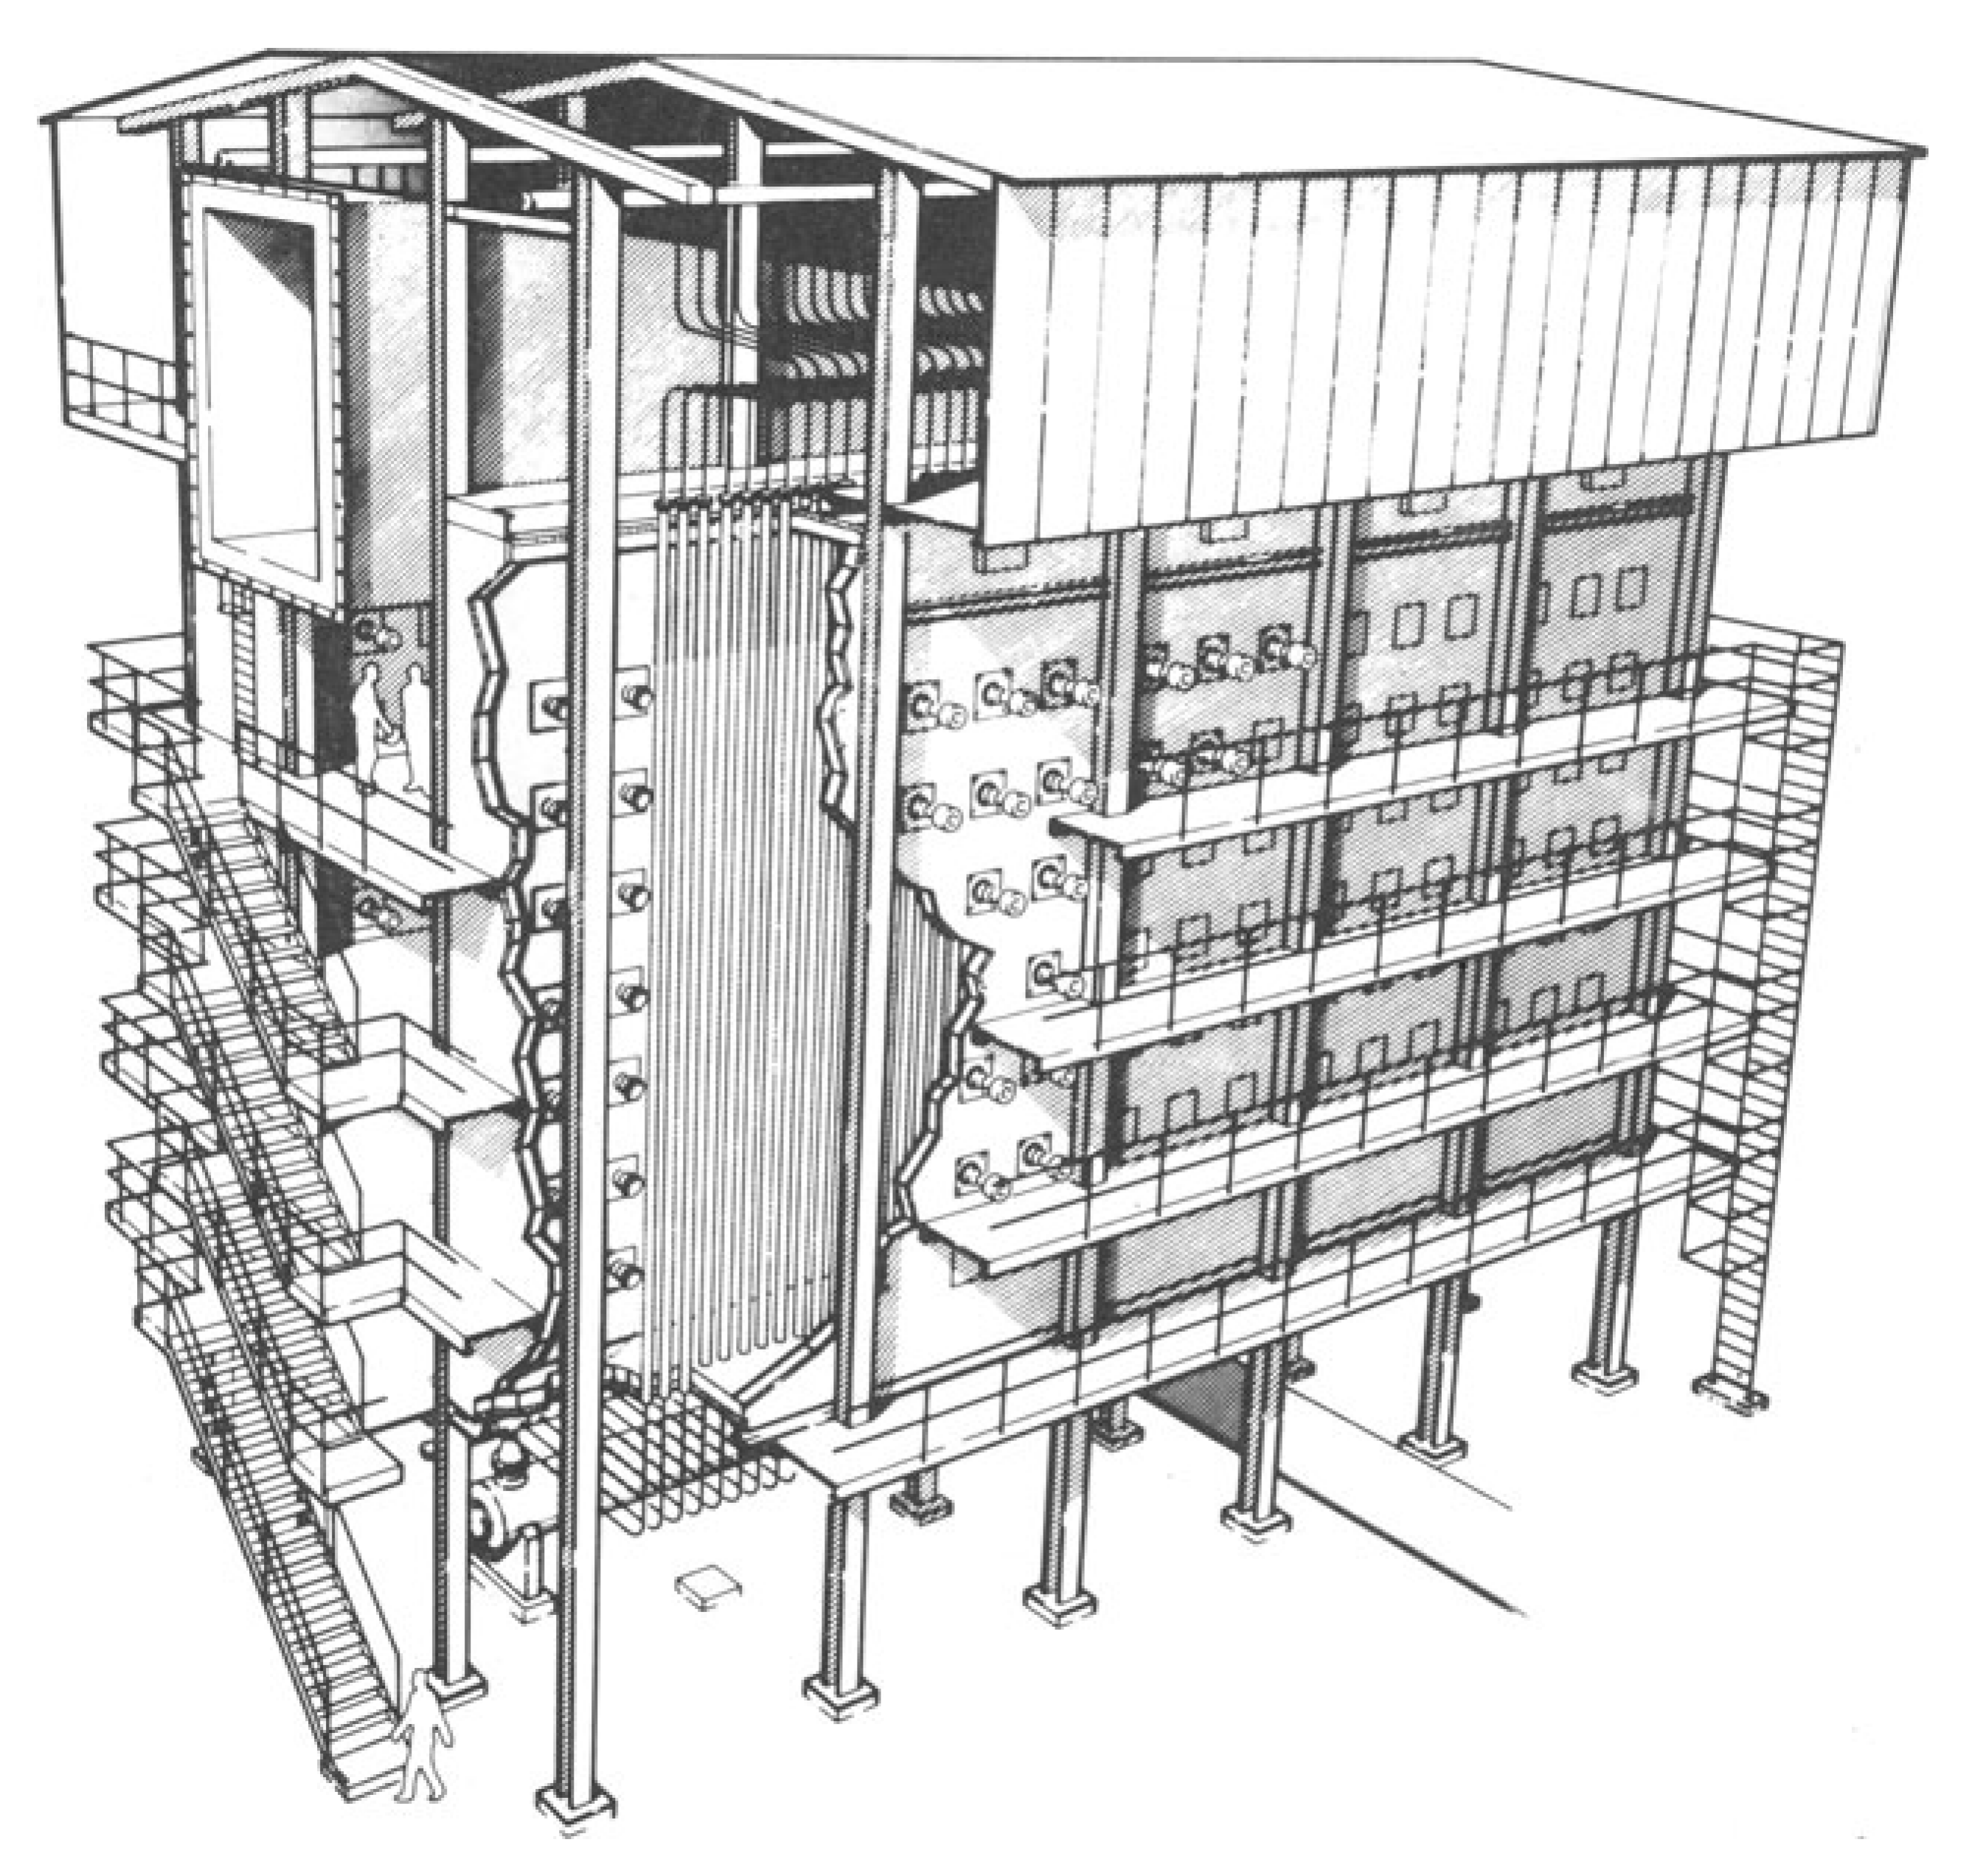
\includegraphics{figures/reformer-furnace}
\caption{Illustration of a typical reformer furnace. The reformer catalyst tubes are arranged vertically, with side-mounted burners on both walls. The pre-heated feedstock gas mixture enters the tubes from the top and the product gas is collected in an outlet manifold at the bottom of the furnace.  From \citet[Fig.~9]{rostrup-nielsen_catalytic_1984}.}
\label{fig:reformer-furnace}
\end{figure}

\begin{figure}[h]
\centering
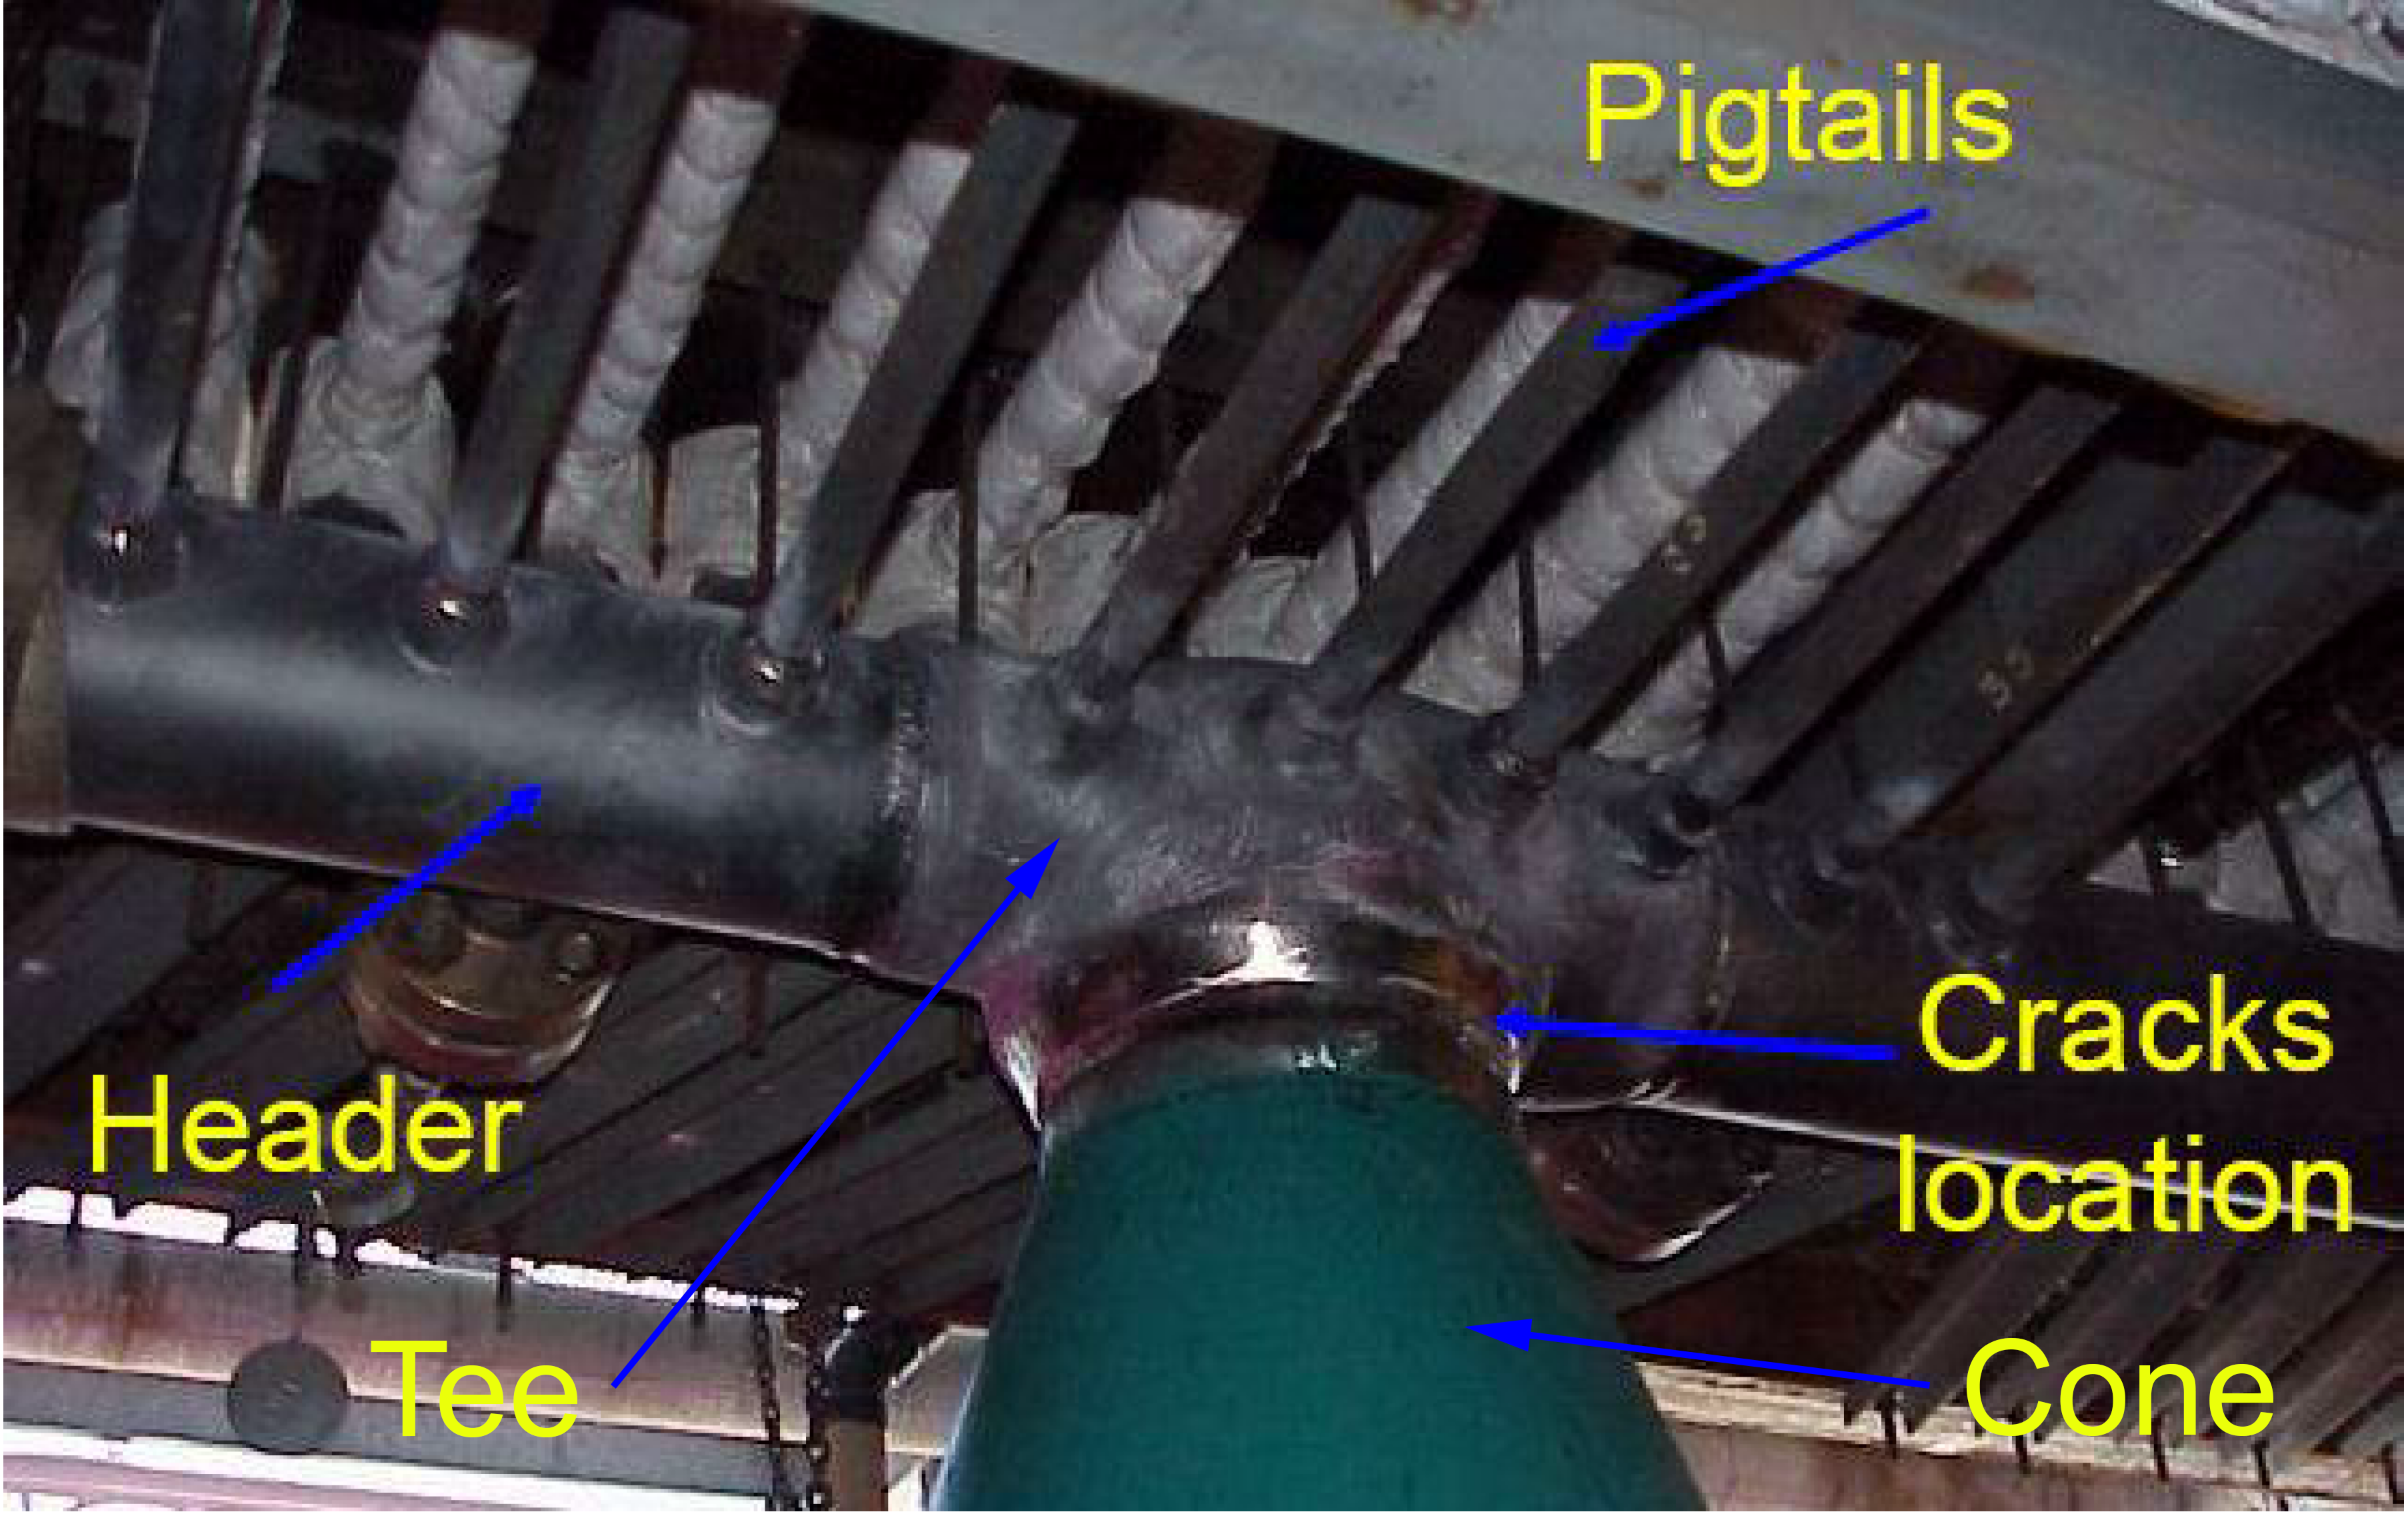
\includegraphics{figures/reformer-tee-cone}
\caption{Photograph of the outlet side of a reformer furnace, showing the outlet pigtails from the reformer catalyst tubes and the outlet header, tee, and cone which connect to the refractory-lined transfer system.  From \citet{penso_repair_2006}.}
\label{fig:reformer-tee-cone}
\end{figure}

Because high exit temperatures maximize the yield of hydrogen from the reformer \cite{haussinger_hydrogen_2000}, typical temperatures are in the range of 700--900C on the outlet side of the reformer furnace. Thus, the reformer tubes and outlet manifold require materials possessing excellent creep performance in addition to resistance to carburization and oxidation. The traditional choice for reformer tubes was centrifugally cast HK-40 (20Cr-25Ni) alloy \cite{rostrup-nielsen_catalytic_1984}, although this has been supplanted by newer alloys such as the HP-Modified alloys (25Cr-35Ni) due to higher creep strength \cite{schillmoller_hp-modified_1992}. For outlet manifold components, Alloy 800, HU-40 (19Cr-39Ni), and HK-40 have been used previously \cite{shibasaki_experience_1993}. The HU-40 and HK-40 alloys were implemented because they offered higher creep strength than Alloy 800, but they were discovered to have problems either with excessive thermal gradients (for HU-40), which was the same problem as originally experienced with Alloy 800, or with unacceptable loss of ductility after long-term service exposure (HK-40) \cite{shibasaki_experience_1993,collins_effect_1980}. To increase the ductilty after service exposure while maintaining high creep strength, a cast steel with the nominal composition of 20Cr-32Ni-Nb was developed \cite{collins_effect_1980}. This alloy, which is specified as Grade CT15C in ASTM A351 \cite{astm_a351_2010}, has similar creep strength to HK-40 \cite{shibasaki_experience_1993} with improved ductility after service-exposure. 

Despite these improvements over traditional alloys, over the years industry has become aware \cite{api_942_2014} that the 20Cr-32Ni-Nb alloy exhibits significant issues when it is subjected to repair welding after service exposure. These issues manifest primarily as cracking occurring in the base metal \gls{haz}, for example as reported by \citet{hoffman_weld_1998}. The cracking occurrences are not alleviated by changes to welding procedures, such as utilizing a more ductile filler metal, but rather are only prevented by high-temperature solution annealing (>2000\textdegree{}F) of the service-exposed material prior to welding. Thus the cracking issues are directly related to the microstructural changes which occur under service conditions (700--900C). The objective of the current work is to evaluate the weldability of service-exposed 20Cr-32Ni-Nb material, utilizing a well-established test method for characterizing the weldability of steels (the Gleeble hot ductility test), and to relate the hot ductility results to observed microstructural characteristics.


% Due to high exit temperatures in the range of 700--900C on the outlet side of the reformer furnace, the reformer tubes and outlet manifold require materials possessing excellent creep performance. 


% Because the efficiency of the reforming reactions are linked to the exit temperature, materials with excellent creep performance are necessary for both the reformer tubes and outlet manifold to enable high operating temperatures to ensure high yield.


% Because the efficiency of the reforming reactions are dependent upon maintaining a high exit temperature, materials with excellent creep performance are necessary for both the reformer tubes and outlet manifold to enable high operating temperatures to ensure high yield.


% how does tube creep properties influence tube design?


% Because the reaction in 1 is endothermic while 2 and 3 are exothermic, the overall heat balance is negative under most process conditions and external heat must be supplied. Thus, steam reforming occurs in a reformer furnace having numerous reformer tubes which contain the catalyst material and through which the reactants are passed. 



    %!TEX root = ..\ms-thesis.tex
\chapter{Literature Review} \label{ch:literature-review}

\section{Weldability Evaluation} \label{sec:weldability-evaluation}

\subsection{Characteristics of a Weldability Test}

\subsection{The Hot Ductility Test}

\subsubsection{Hot Ductility Evaluation Criteria}
In one of their early studies utilizing the Gleeble hot ductility test to evaluate a number of alloys, \citet{nippes_further_1957} classified the observed hot ductility responses of the various alloys into several categories, based on the shapes of the hot ductility curves: Classes H1 or H2 for the on-heating behavior and Classes C1, C2, or C3 for the on-cooling behavior. Schematic hot ductility curves illustrating the characteristics of each behavior class are shown in Figure~\ref{fig:nippes-criteria} and a brief text description for each is provided in Table~\ref{tab:nippes-classification}. Of the two on-heating behavior categories, Class H2 (Figure~\ref{fig:nippes-criteria}b) behavior was identified as being intrinsically sensitive to hot cracking. Class H1 behavior (Figure~\ref{fig:nippes-criteria}a) was not considered in and of itself indicative of a propensity for hot cracking and thus required the evaluation of on-cooling results to determine the material's susceptibility. With regard to the on-cooling categories, materials exhibiting Class C1 (Figure~\ref{fig:nippes-criteria}c) behavior were considered not sensitive to hot cracking. Class C2 and Class C3 behaviors (Figure~\ref{fig:nippes-criteria}d,e) were associated with a higher sensitivity to hot cracking, with Class C3 behavior indicating the greatest sensitivity. In particular, \citeauthor{nippes_further_1957} found that those materials in the study which were known to exhibit hot cracking, based on field experience, exhibited Class C3 behavior with on-cooling ductility of 40\% or less of the on-heating ductility. Thus, using the Nippes classification system, in most cases a material's on-cooling ductility response will be the major indicating factor regarding its hot cracking susceptibility. Materials exhibiting Class C3 on-cooling behavior with a low recovery of on-cooling ductility (0--40\% of on-heating ductility) can be identified as showing the greatest susceptibility to hot cracking.

% Nippes Criteria
%\bigskip
\begin{figure}[h]
\centering
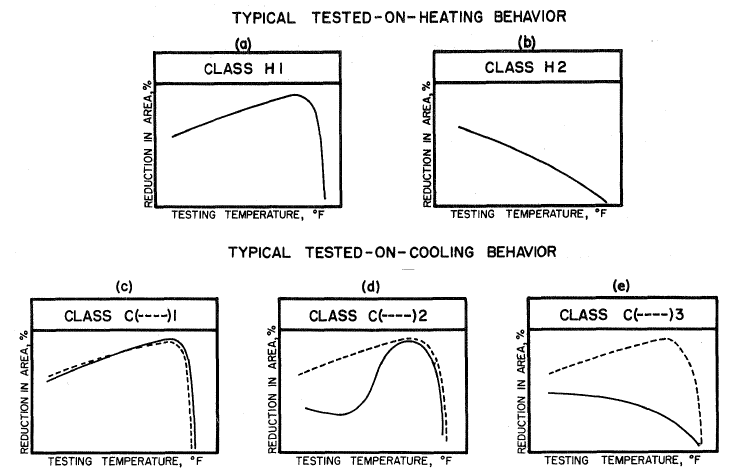
\includegraphics[width=6in]{figures/nippes-criteria.png}
\caption{Classification of Hot Ductility Behavior for On-heating and On-Cooling Tests; in (c), (d), and (e), the solid line is the on-cooling curve and the dashed line is the on-heating curve.  From \citet[Fig.~66]{nippes_further_1957}.}
\label{fig:nippes-criteria}
\end{figure}

\begin{table}[h]
\caption{Classification of on-heating and on-cooling hot ductility responses based on the work of \citet{nippes_further_1957}. Schematic curves for each behavior class are depicted in Figure~\ref{fig:nippes-criteria}.}
\begin{tabular}{ lp{4in} }
\toprule
\textbf{Classification} & \textbf{Description} \\
\midrule
On-Heating Class H1 & On-heating ductility generally increases as temperature increases, followed by a sudden loss of ductility over a relatively narrow range as the temperature increases further toward the melting point. (Figure~\ref{fig:nippes-criteria}a) \\
\addlinespace
On-Heating Class H2 & On-heating ductility shows a gradual decrease over a wide temperature range as the temperature increases toward the melting point. (Figure~\ref{fig:nippes-criteria}b) \\
& \\
On-Cooling Class C1 & On-cooling ductility is the essentially same as on-heating ductility at all test temperatures. (Figure~\ref{fig:nippes-criteria}c) \\
\addlinespace
On-Cooling Class C2 & On-cooling ductility is the same as on-heating ductility at test temperatures of 2100\textdegree{}F or above, but is significantly lower at test temperatures in the range of 1800--2000\textdegree{}F. (Figure~\ref{fig:nippes-criteria}d) \\
\addlinespace
On-Cooling Class C3 & On-cooling ductility is lower than on-heating ductility at all test temperatures; severity of ductility decrease may change with on-cooling test temperature or with the peak temperature utilized for the on-cooling thermal cycle. (Figure~\ref{fig:nippes-criteria}e) \\
\bottomrule
\end{tabular}
\label{tab:nippes-classification}
\end{table}


Further investigation of hot ductility test criteria was undertaken in a review by \citet{yeniscavich_correlation_1970}. One of the criteria reviewed, attributed to Nippes, was the \gls{drr}. According to this criteria, crack-resistant materials show a rapid recovery of on-cooling ductility after exposure to the \gls{haz} peak temperature, while the on-cooling ductility for crack-sensitive materials recovers slowly and remains low even at test temperatures well below the peak temperature. Schematic curves illustrating the \gls{drr} for crack-resistant and crack-sensitive materials are shown in Figure~\ref{fig:drr-schematic}. Numerically, the \gls{drr} is determined by taking the ratio of the on-cooling ductility to the on-heating ductility at a specified temperature, typically the rapid-ductility-decrease temperature on the on-heating curve (the point on the curve immediately prior to the sudden drop in ductility).

\begin{figure}
\centering
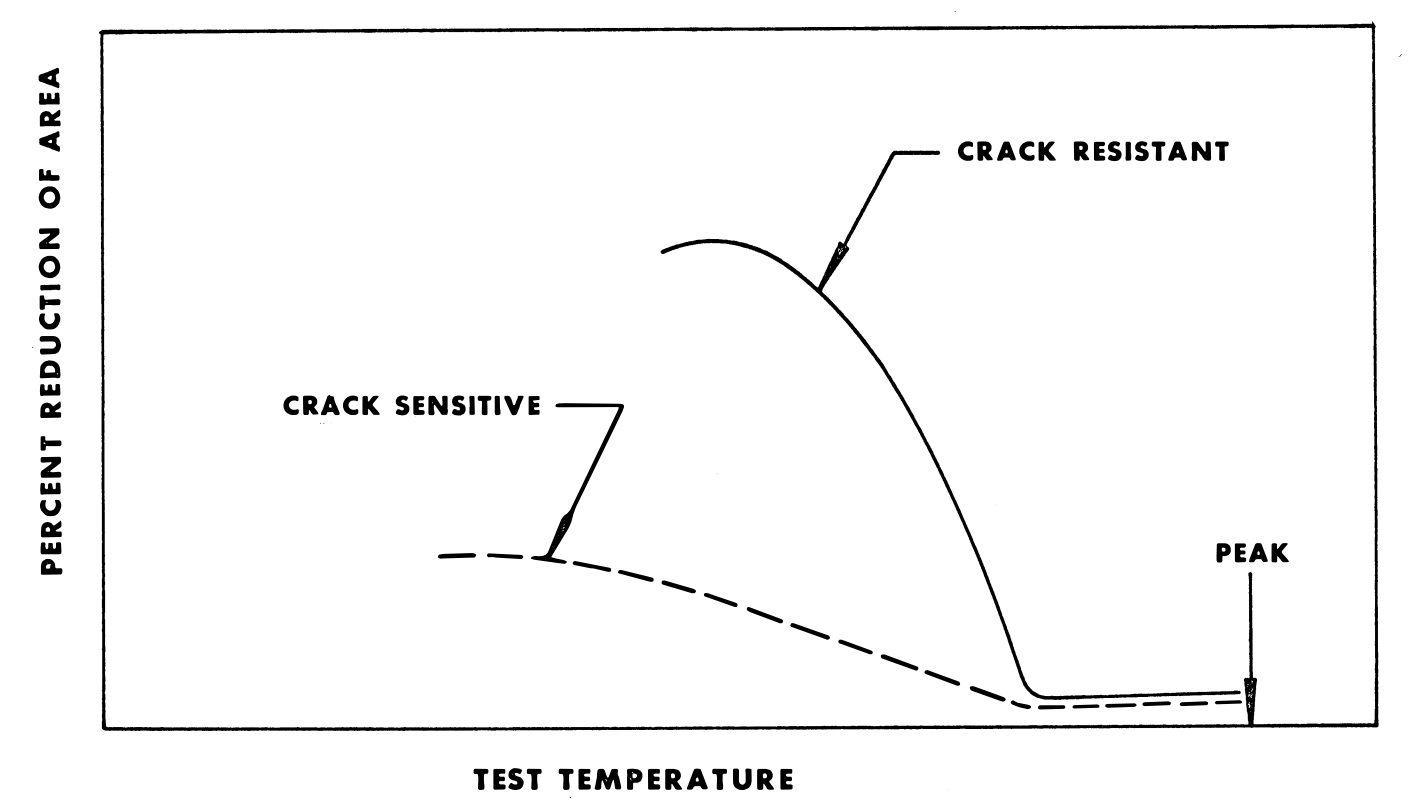
\includegraphics[width=6in]{figures/yeniscavich-drr.png}
\caption{Schematic curves illustrating the on-cooling \acrshort{drr} criteria for crack-resistant and crack-sensitive materials.  From \citet[Fig.~2]{yeniscavich_correlation_1970}}
\label{fig:drr-schematic}
\end{figure}

Yeniscavich also proposed the \gls{zdr} as an improved indicator of propensity for hot cracking. The \gls{zdr} phenomenon corresponds to a finite temperature increment below the ZDT in which the on-cooling ductility remains zero, i.e. the ductility does not immediately increase once the on-cooling test temperature is below the ZDT. The physical significance of the \gls{zdr} is related to the fact that the HAZ must possess sufficient ductility to withstand the thermal strains imposed during welding, otherwise cracking will occur. Since the magnitude of these strains is small over the length scale of an HAZ, the HAZ ductility must be on the order of zero for hot cracking to be of concern. Thus, alloys which show a large \gls{zdr} (zero ductility over a wide on-cooling temperature range) are considered more vulnerable to hot cracking than alloys which show a narrow \gls{zdr} (see Figure~\ref{fig:zdr-schematic}).

\begin{figure}
\centering
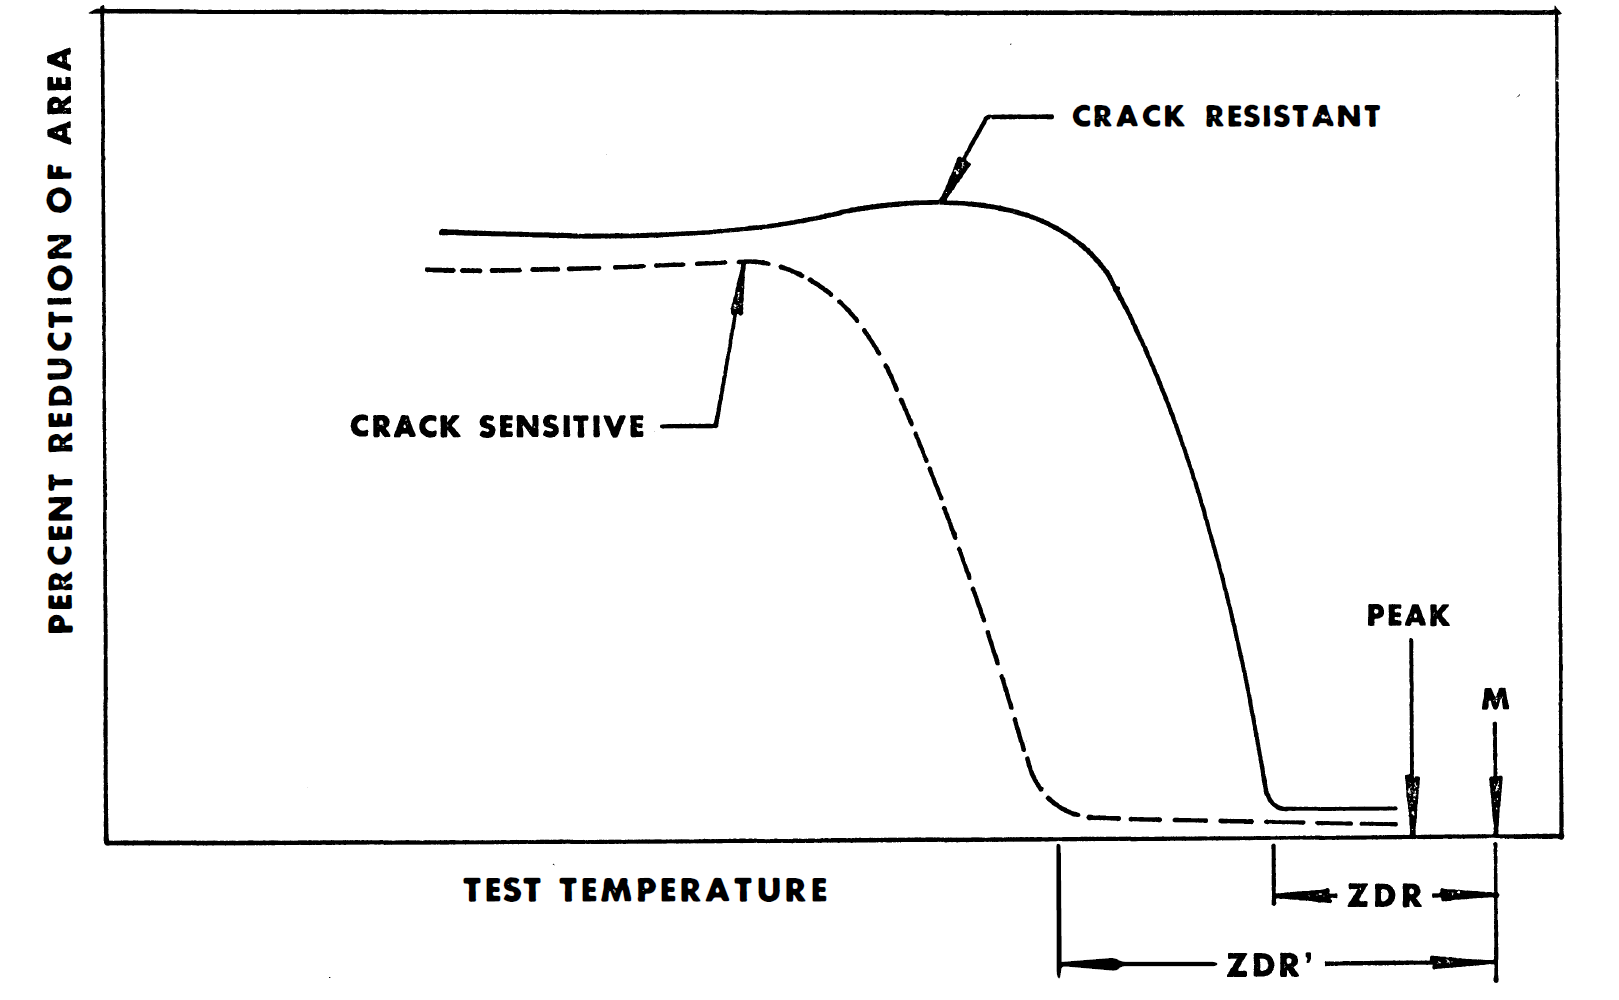
\includegraphics[width=6in]{figures/zdr-schematic.png}
\caption[Schematic of Hot Ductility Curves Illustrating Different On-Cooling Behaviors According to the Zero Ductility Range Criteria.]{Schematic of Hot Ductility Curves Illustrating Different On-Cooling Behaviors According to the Zero Ductility Range Criteria: Crack-Sensitive (\gls{zdr}') and Crack-Resistant (\gls{zdr}).  From \citet[Fig.~4]{yeniscavich_correlation_1970}}
\label{fig:zdr-schematic}
\end{figure}



    \chapter{Computational Fluid Dynamics}\label{ch:cfd}
    %!TEX root = ..\ms-thesis.tex
\chapter{Experimental Methods} \label{ch:experimental-methods}

\section{Hot Ductility Tests}
Standard hot ductility samples with dimensions of 114\,mm (4.5\,in) [length] by 6.35\,mm (0.25\,in) [diameter] were extracted from the Cone~1 and Cone~5 base metals adjacent to the respective cone-to-tee weld joints where cracking during repair welding had been observed.  A thermal cycle characteristic of \gls{smaw} with \SI[round-mode=places,round-precision=2]{2.75}{\kilo\joule\per\milli\meter} (\US{70}{\kilo\joule\per\inch}) energy input in 38\,mm (1.5\,in) stainless steel plate \cite{nippes_heat-affected_1955}, with an initial plate temperature of \SmartUnit{fahrenheit=80}, was utilized for the on-heating hot ductility tests.  This thermal cycle was determined based on the F(s,d) method \cite{nippes_cooling_1949} using data provided by Duffers Scientific \cite{duffers_haz_1989}. The peak temperature of the chosen thermal cycle was \SmartUnit{fahrenheit=2450}, equal to the estimated solidus temperature for the CT15C alloy based on data for Incoloy 800H (CT15C is considered a ``cast'' version of 800H) and which would roughly correspond to the maximum temperature experienced at the weld fusion line.

Once the on-heating hot ductility tests had been performed using the aforementioned thermal cycle and the \gls{zdt} had been determined, the thermal cycle was re-scaled so that the peak temperature coincided with the \gls{zdt}. The modified thermal cycle was subsequently used to perform the on-cooling hot ductility tests.  Both the on-heating and on-cooling tests were conducted according to the parameter guidelines recommended by a detailed study \cite{lundin_standardization_1990_experiment} undertaken to establish a standardized procedure for hot ductility testing.  The specific test parameters utilized in the current work are given in Table~\ref{tab:hot-ductility-parameters}.  For each test, the output of the control thermocouple was recorded, and the post-test cross-sectional area was determined and used to calculate the ductility in terms of percent reduction in area for each specimen.  The collected data were used to create plots of on-heating and on-cooling ductility (\% RA) as a function of test temperature.

\begin{table}[h]
\caption{Parameters and Conditions Used for Hot Ductility Testing, Based on Recommendations in \citet{lundin_standardization_1990_experiment}}
\begin{tabular}{ lp{4in} }
\toprule
\textbf{Parameter} & \textbf{Condition} \\
\midrule
Thermal Cycle & 38\,mm (1.5\,in) stainless steel plate, \gls{smaw} process, \SI[round-mode=places,round-precision=2]{2.75}{\kilo\joule\per\milli\meter} (\US{70}{\kilo\joule\per\inch}) energy input, \SmartUnit{fahrenheit=80} initial plate temperature \\
\addlinespace
Sample & 114\,mm (4.5\,in) length, 6.35\,mm (0.25\,in) diameter, 1/4-20 thread \\
\addlinespace
On-Cooling Peak Temp. & Zero Ductility Temperature determined from On-Heating Curve \\
\addlinespace
Crosshead Speed & \SI{50}{\milli\meter\per\second} (\US{2}{\inch\per\second}) \\
\addlinespace
Jaw Separation & 16\,mm (0.625 in) \\
\addlinespace
Control Thermocouple & 0.25\,mm (0.01\,in) diameter Chromel-Alumel; Percussion Welding / Separate attachment technique, \SI{1}{\milli\metre} wire spacing \\
\addlinespace
%Preload & \SIrange{3}{4}{\kilo\newton} \\
Test Atmosphere & Air \\
\bottomrule
\end{tabular}
\label{tab:hot-ductility-parameters}
\end{table}

\section{Microstructure Characterization}
Metallographic evaluations were conducted for the as-received Cone~1 and Cone~5 materials, utilizing remnants of the slices removed from the cones for machining of the hot ductility samples.  Metallography was also performed on selected hot ductility samples.  The hot ductility samples were sectioned longitudinally and mounted in castable epoxy and were subsequently ground and polished to a \SI[round-mode=places,round-precision=2]{0.05}{\micro\meter} finish.  The polished samples were electrolytically etched with an aqueous 10\% oxalic acid solution using a stainless steel cathode (\SI{50}{\milli\meter} (\US{2}{\inch}) spacing between the sample and cathode). For the as-received base metal samples, a potential of \SI{6}{\volt} for \SIrange[range-phrase=--]{3}{5}{\second} was used; for the hot ductility samples, it was found that a lower potential, \SI[round-mode=places,round-precision=1]{1.5}{\volt} for \SI{3}{\second}, was necessary to avoid excessive attack of certain phases near the fracture surfaces. \Gls{olm} examination of the etched samples was performed with a Nikon MA-200 inverted metallograph equipped with a 12 megapixel digital camera for obtaining micrographs. \Gls{sem} examination was conducted on selected samples using a LEO Gemini 1525 field emission \gls{sem} equipped with an Oxford Instruments PentaFet \gls{eds} system. Typically, a beam voltage of \SI{20}{\kilo\volt} was used for both \gls{se} and \gls{bse} imaging and for \gls{eds} analysis.
    %!TEX root = ..\ms-thesis.tex
\chapter{Results and Discussion} \label{ch:results-discussion}

\section{Hot Ductility Curves}
The on-heating and on-cooling hot ductility curves for the Cone~1 and Cone~5 materials are presented in Figure~\ref{fig:c1-hot-ductility} and Figure~\ref{fig:c5-hot-ductility} respectively.  In general, the on-heating ductility for both Cones increased with testing temperature, up to a ductility maximum, before dropping rapidly to zero over a short temperature range.  From Figure~\ref{fig:c1-hot-ductility} and Figure~\ref{fig:c5-hot-ductility}, it is apparent that Cone~1 and Cone~5 also showed similar trends in on-cooling behavior, in that the on-cooling ductility remains essentially zero for a definite temperature range below the \gls{zdt} before gradually increasing at lower test temperatures.  Specifically for Cone~1, it is apparent from Figure~\ref{fig:c1-hot-ductility} that the Cone~1 material exhibited an on-heating \gls{zdt} of 2375\textdegree{}F and an on-cooling \gls{drt} of 2300\textdegree{}F, resulting in a \gls{zdr} of 75F\textdegree{}.  Figure~\ref{fig:c5-hot-ductility} shows that the Cone~5 material also exhibited an on-heating \gls{zdt} of 2375\textdegree{}F, \gls{drt} of 2300\textdegree{}F, and \gls{zdr} of 75F\textdegree{}.  These characteristics of the hot ductility curves for both materials are summarized in Table~\ref{tab:hot-ductility-results}.

\begin{figure}[h!]
    \setlength{\abovecaptionskip}{15pt}
    \centering
    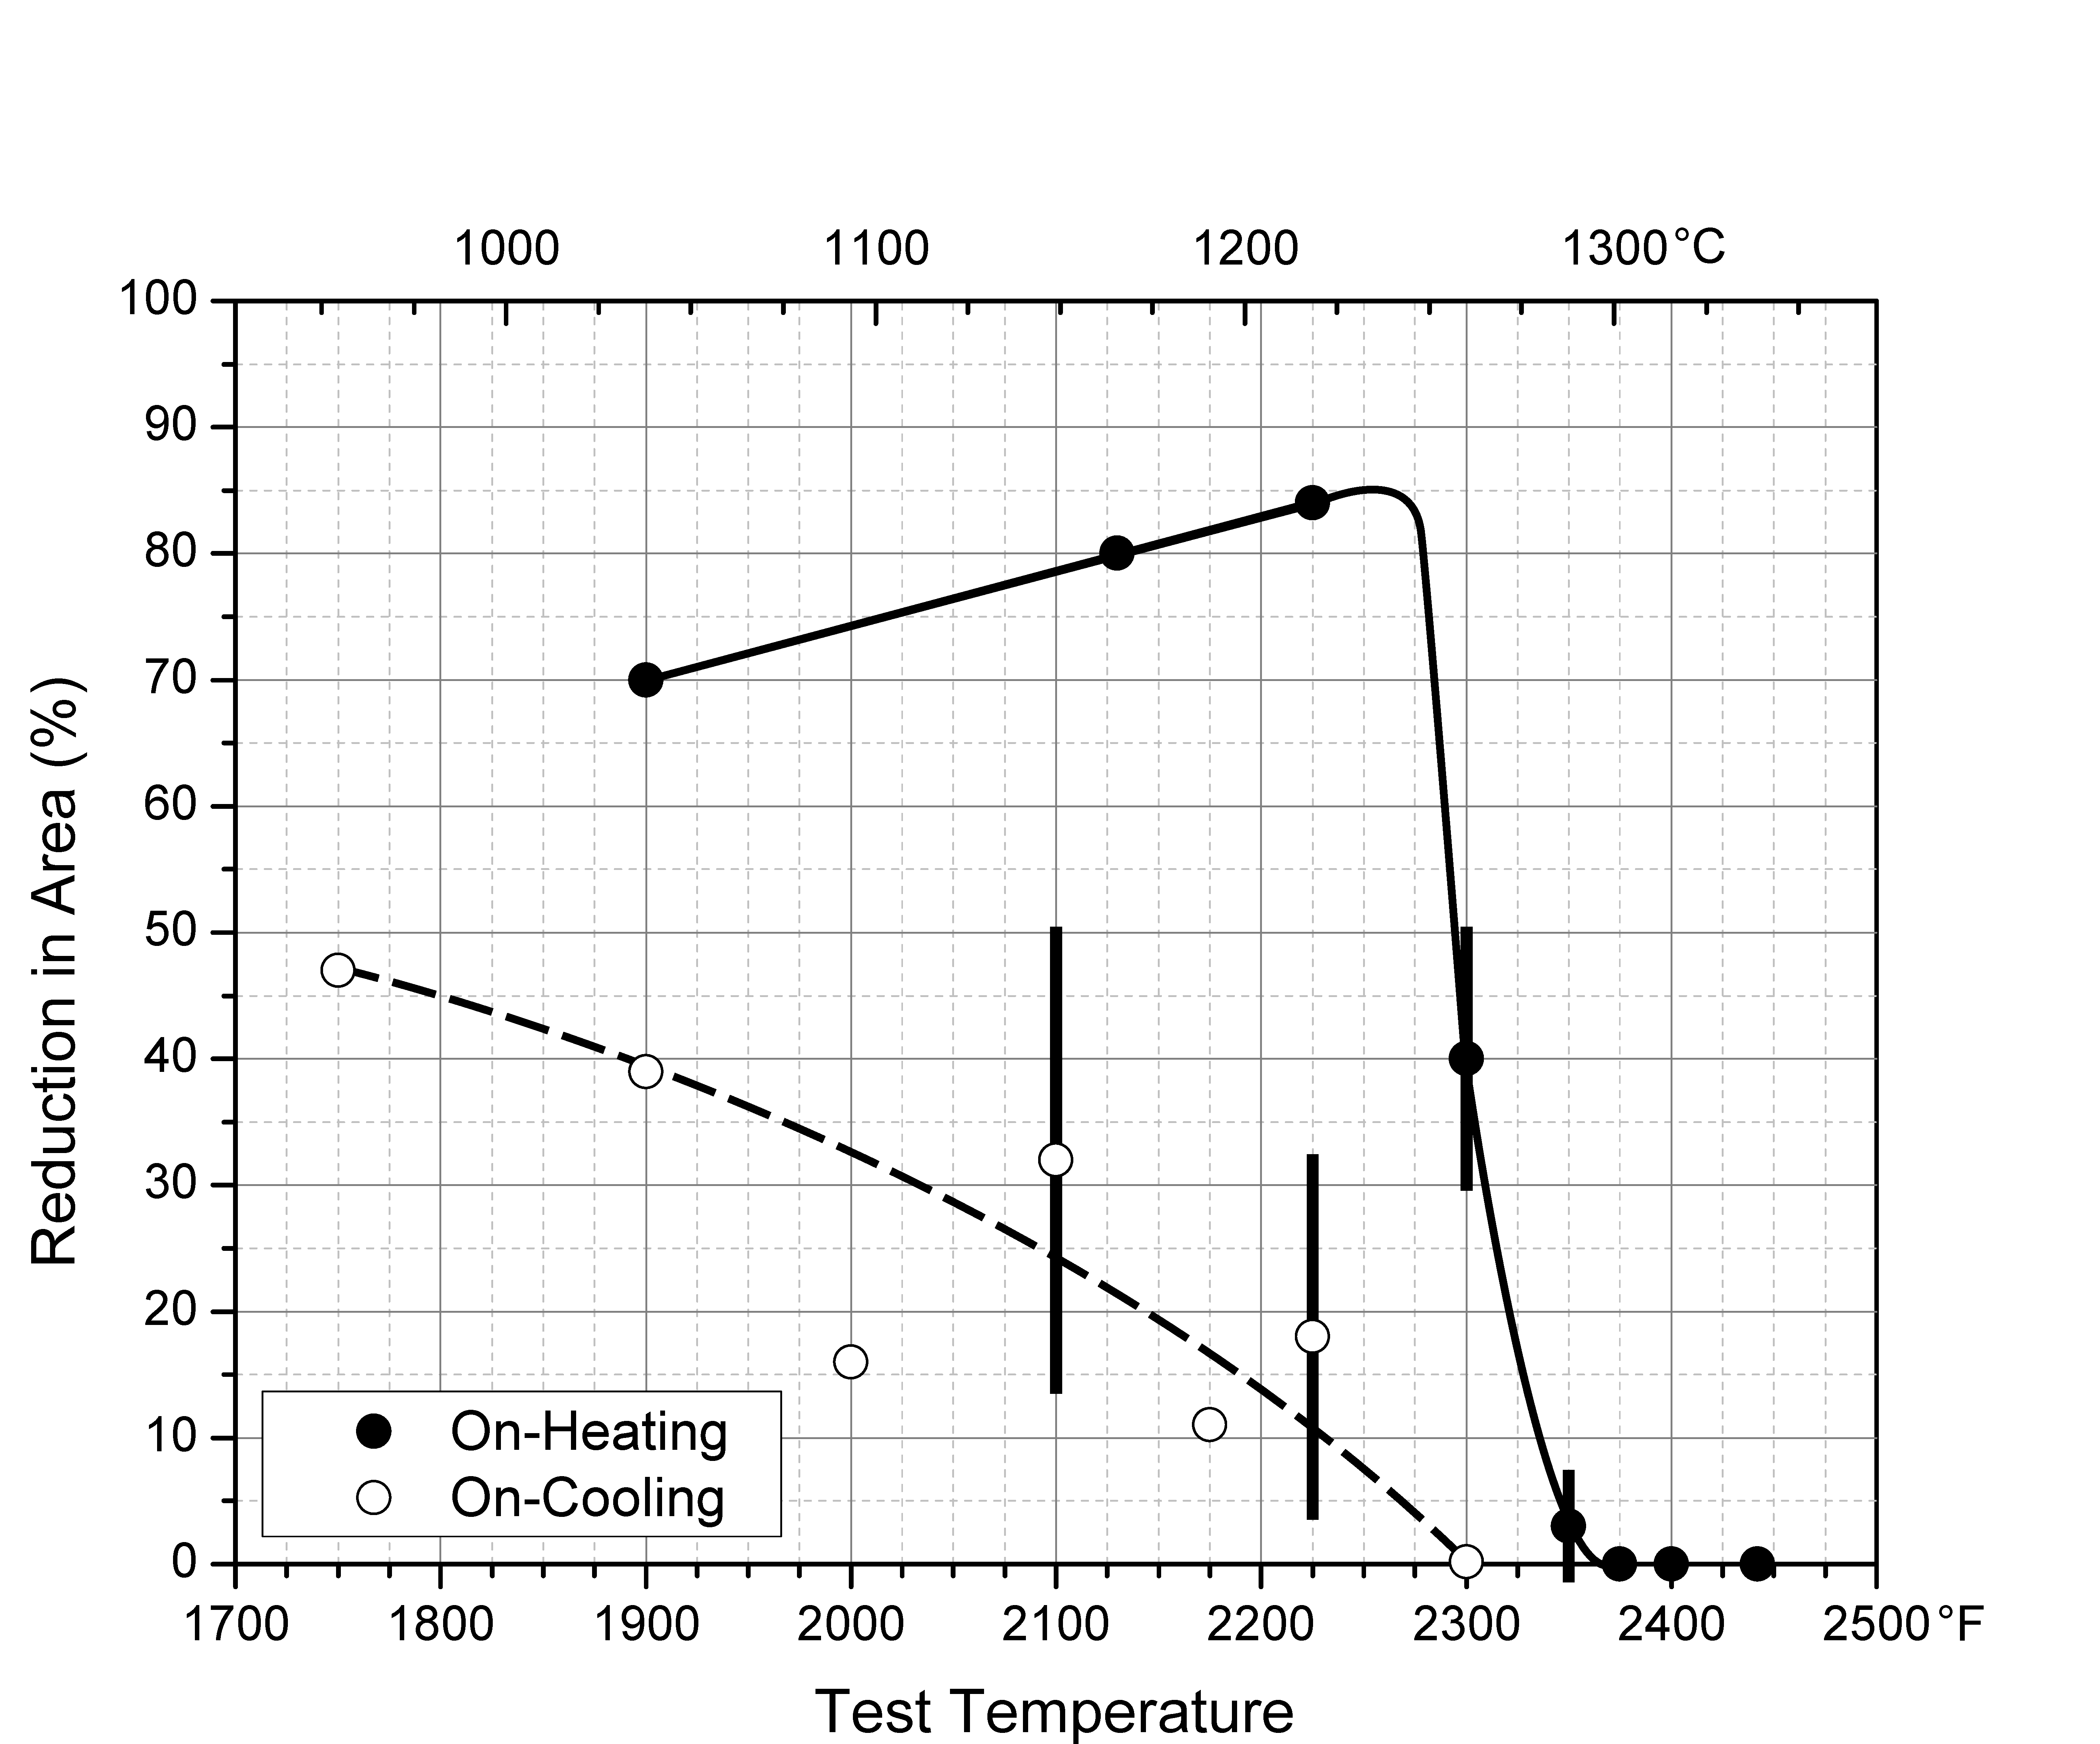
\includegraphics[width=6in]{figures/hot-ductility/c1-hot-ductility-curve.pdf}
    \caption[Hot Ductility Behavior of Cone~1 Base Metal.]{Hot Ductility Behavior of CT15C Cone~1 Base Metal.  Bars indicate range of \%RA values at indicated test temperature.  On-Heating Curve Exhibits Class H1 behavior with \gls{zdt} = 2375\textdegree{}F; On-Cooling Curve (from Peak Temperature of 2375\textdegree{}F) Exhibits Class C3 behavior.  \gls{drr}(2225\textdegree{}F) = 21\%. Hot Ductility Test Parameters Given in Table~\ref{tab:hot-ductility-parameters}.}
    \label{fig:c1-hot-ductility}
\end{figure}

\begin{figure}[h!]
    \setlength{\abovecaptionskip}{15pt}
    \centering
    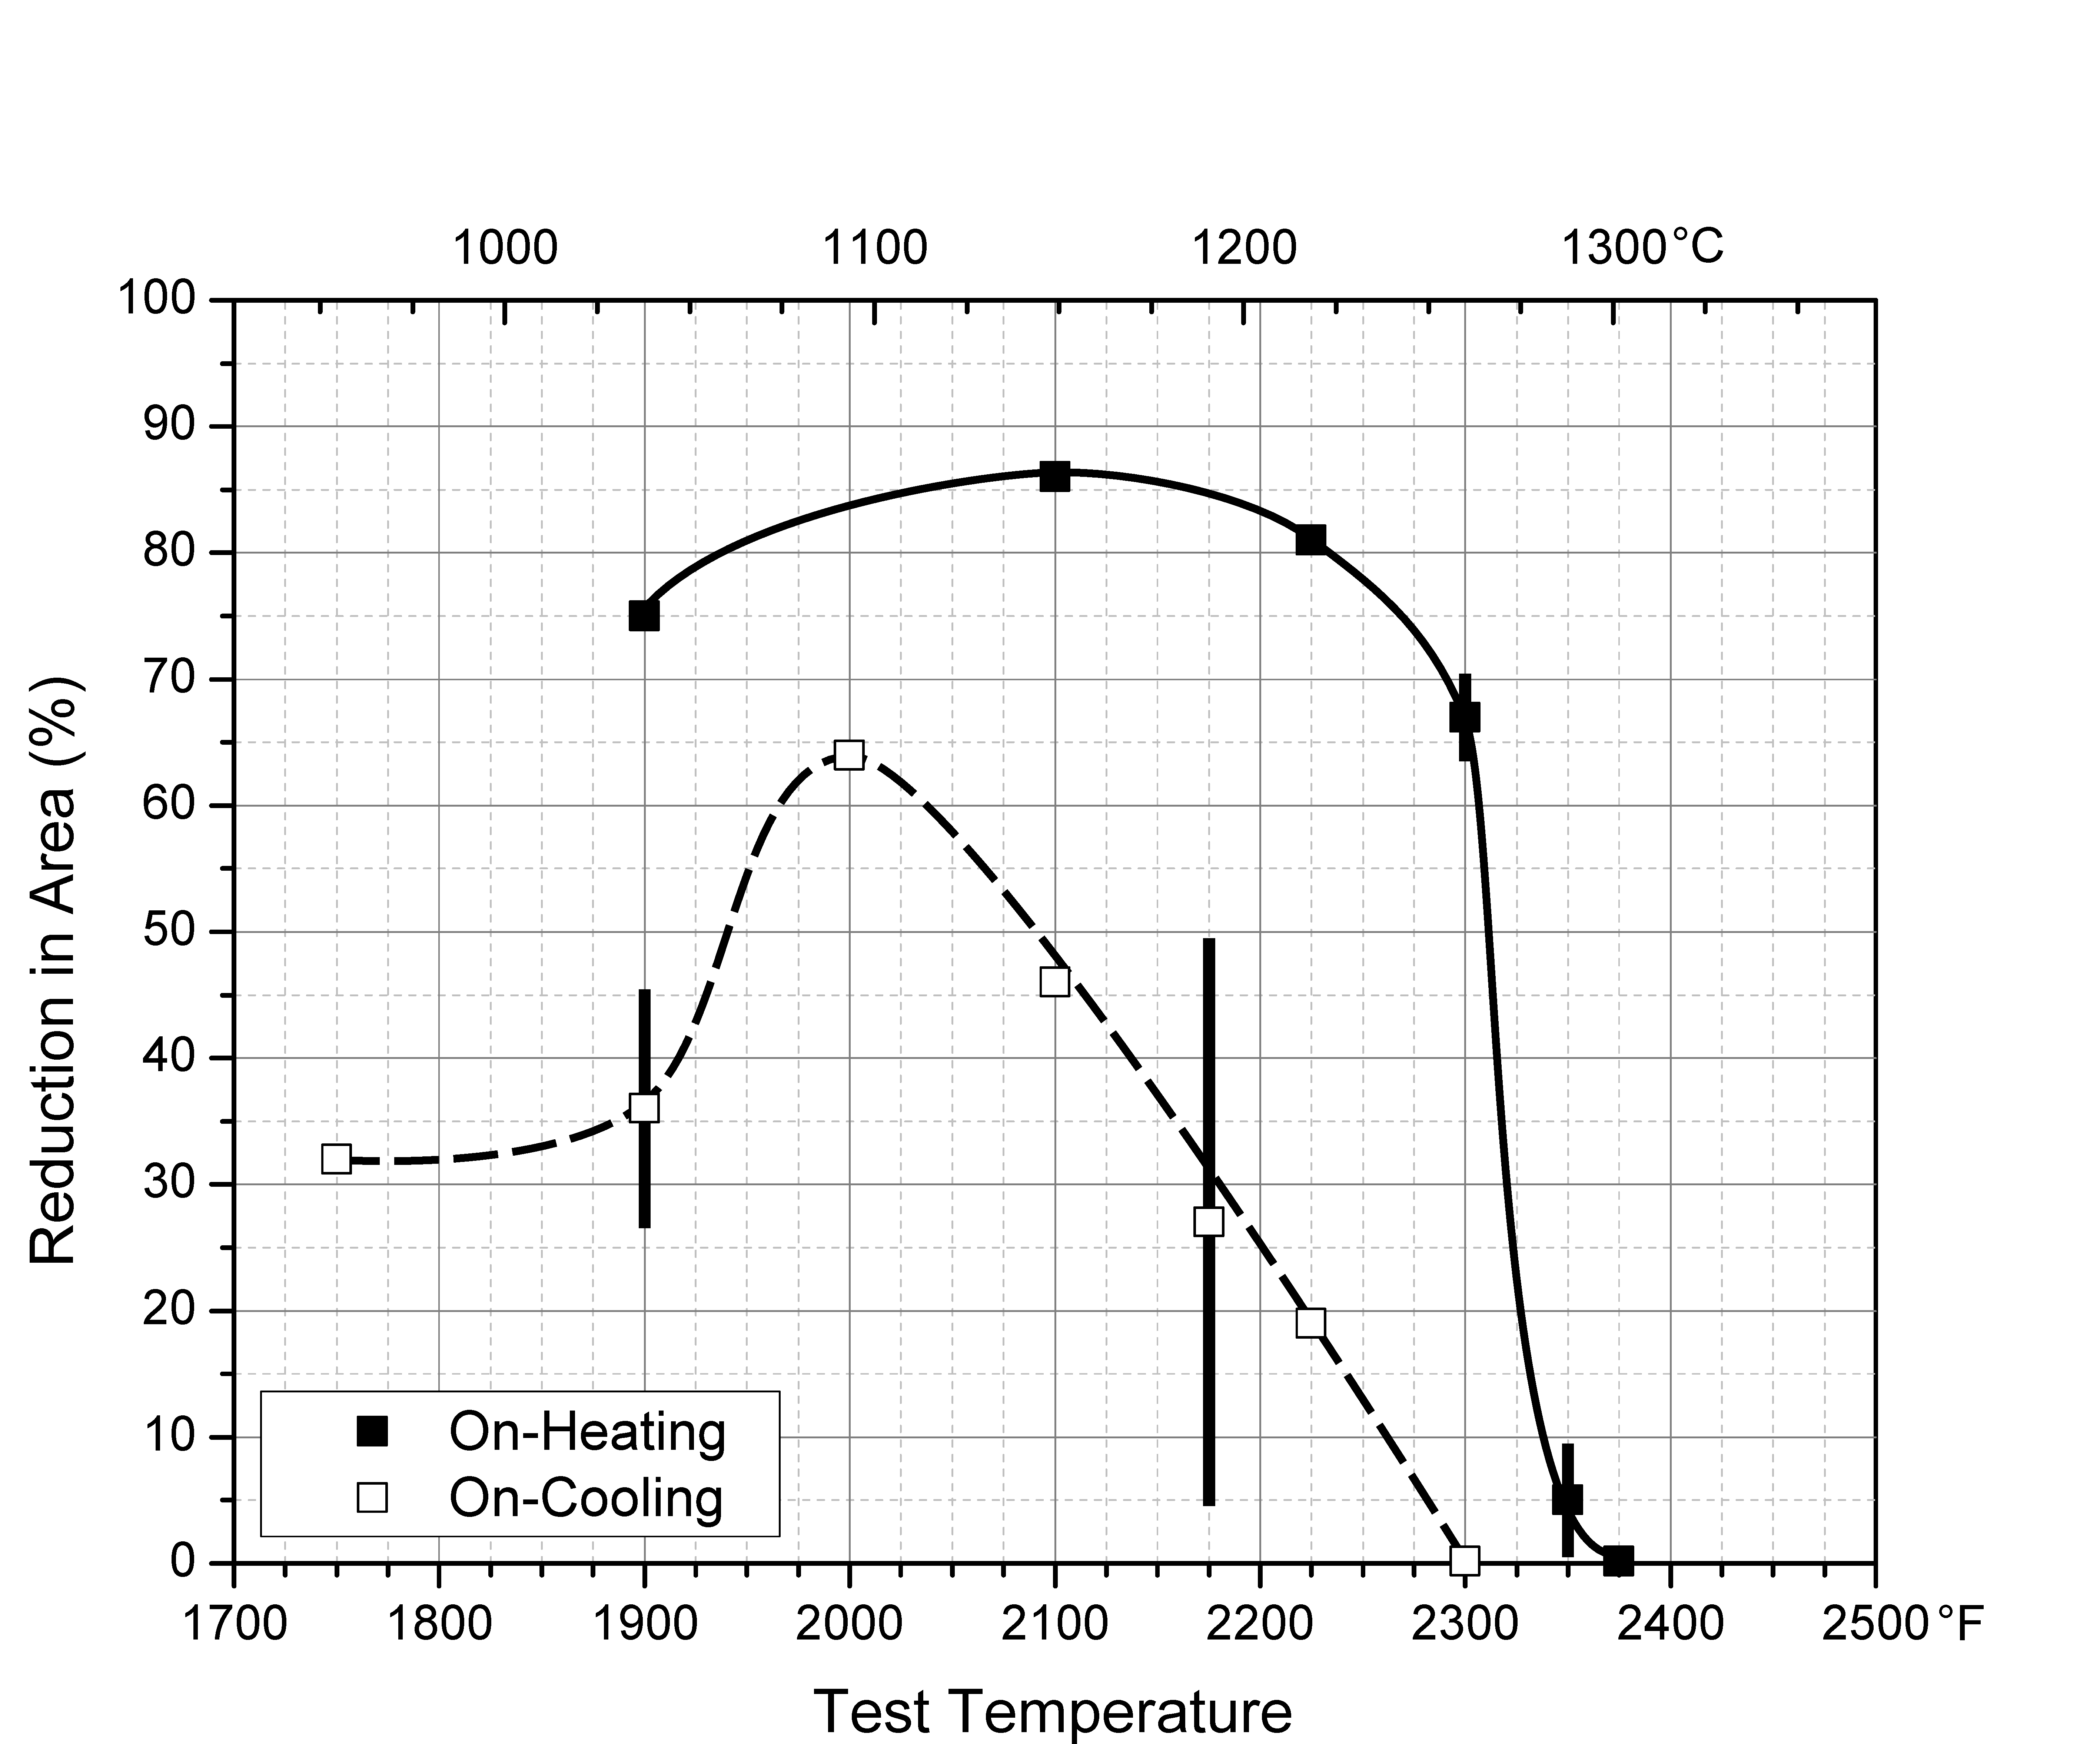
\includegraphics[width=6in]{figures/hot-ductility/c5-hot-ductility-curve.pdf}
    \caption[Hot Ductility Behavior of Cone~5 Base Metal.]{Hot Ductility Behavior of CT15C Cone~5 Base Metal.  Bars indicate range of \%RA values at indicated test temperature.  On-Heating Curve Exhibits Class H1 behavior with \gls{zdt} = 2375\textdegree{}F; On-Cooling Curve (from Peak Temperature of 2375\textdegree{}F) Exhibits Class C3 behavior.  \gls{drr}(2225\textdegree{}F) = 23\%. Hot Ductility Test Parameters Given in Table~\ref{tab:hot-ductility-parameters}.}
    \label{fig:c5-hot-ductility}
\end{figure}

\begin{table}[h]
    \caption{Summary of hot ductility characteristics for Cone~1 and Cone~5 materials, as determined from the curves in Figure~\ref{fig:c1-hot-ductility} and Figure~\ref{fig:c5-hot-ductility}.}
    \begin{tabular}{ lccc }
    \toprule
    \textbf{Material ID and Condition} & \textbf{\gls{zdt} (\textdegree{}F)} & \textbf{\gls{drt} (\textdegree{}F)} & \textbf{\gls{zdr} (\gls{zdt}-\gls{drt}) (F\textdegree{})} \\
    \midrule
    Cone~1 & 2375 & 2300 & 75 \\
    Cone~5 & 2375 & 2300 & 75 \\
    \bottomrule
    \end{tabular}
    \label{tab:hot-ductility-results}
\end{table}
\clearpage

As can be seen from Figure~\ref{fig:c1-hot-ductility} and Figure~\ref{fig:c5-hot-ductility}, the on-heating hot ductility curves for both Cone materials appear similar, with similar reduction in area (\% RA) values at each test temperature, except in the vicinity of 2300\textdegree{}F.  At this temperature, Cone~1 exhibits a more rapid loss in ductility than Cone~5.  Based on the Nippes evaluation criteria \cite{nippes_further_1957} described previously, examination of the shape of the on-heating ductility curves in Figure~\ref{fig:c1-hot-ductility} and Figure~\ref{fig:c5-hot-ductility} shows that both Cones exhibit Class H1 on-heating hot ductility behavior rather than Class H2 behavior.  This observation regarding the Cone~1 and Cone~5 materials is indeterminate on its own, as \citet{nippes_further_1957} observed in some cases that two materials which both showed H1 on-heating behavior were later found to exhibit either crack-sensitive or crack-insensitive characteristics when tested on-cooling.

Considering the shapes of the on-cooling ductility curves for the Cone~1 and Cone~5 materials after exposure to a peak temperature corresponding to the on-heating \gls{zdt} (2375\textdegree{}F) as shown Figure~\ref{fig:c1-hot-ductility} and Figure~\ref{fig:c5-hot-ductility}, it is apparent that both Cone materials exhibit Class C3 on-cooling behavior when exposed to the \gls{zdt}, based on the Nippes criteria (Figure~\ref{fig:nippes-criteria}).  This category of on-cooling behavior is associated with the greatest degree of hot cracking susceptibility as established by \citet{nippes_further_1957}.  While in general both materials exhibit Class C3 behavior, it appears from Figure~\ref{fig:c1-hot-ductility} and Figure~\ref{fig:c5-hot-ductility} that Cone~5 shows a slightly better qualitative recovery of on-cooling ductility than Cone~1.  As shown in Figure~\ref{fig:c5-hot-ductility}, the on-cooling ductility for Cone~5 recovers to higher values than for Cone~1, particularly at 2100\textdegree{}F and 2000\textdegree{}F.  However, when considering the apparent difference, it should be noted that both Cones are cast components with a large dendrite size, and it was observed in early work on hot ductility by \citet{nippes_further_1957} that castings typically showed wider variation in ductility values at a given test temperature than was observed for wrought material.  The 20Cr-32Ni-1Nb cast material used in both Cones is no different in this regard, for example as evidenced by the variation at 2100\textdegree{}F on-cooling for Cone~1 and 2175\textdegree{}F on-cooling for Cone~5.  Due to the reality of variations in ductility values, it is recommended practice (\citet{lundin_standardization_1990_experiment}) to run a minimum of two hot ductility tests at each temperature, with some studies (\citet{nippes_further_1957}) running up to four tests per temperature for cast materials.  Unfortunately, the number of samples available in the current study was not sufficient to permit duplicate tests at all test temperatures; however, duplicates were performed wherever possible, including at the \gls{zdt}.  If sufficient samples had been available for duplicate tests at all temperatures, it is possible that the average \% RA at certain test temperatures (e.g. 2000\textdegree{}F on-cooling and 2100\textdegree{}F on-cooling) would be closer in magnitude between Cone~1 and Cone~5.  Taking these considerations into account, it is likely that Cone~1 and Cone~5 are more similar in on-cooling behavior than would be suggested by a casual inspection of the curves in Figure~\ref{fig:c1-hot-ductility} and Figure~\ref{fig:c5-hot-ductility}.

To quantify the severity of the on-cooling ductility loss exhibited by both materials, the ductility recovery rate (\gls{drr}) was determined for both Cone~1 (Figure~\ref{fig:c1-hot-ductility}) and Cone~5 (Figure~\ref{fig:c5-hot-ductility}) at a test temperature of 2225\textdegree{}F since this corresponds most closely with the observed rapid-ductility-decrease temperature (on-heating) for both Cones.  The \gls{drr} at 2225\textdegree{}F was similarly low for both Cone materials: 21\% for Cone~1 and 23\% for Cone~5.  Additionally, both Cones exhibited a region of zero on-cooling ductility (\gls{zdr}) after exposure to the on-heating \gls{zdt}; for both Cone~1 and Cone~5, the \gls{zdr} is 75F\textdegree{} wide (2300–2375\textdegree{}F).  Considered together, the occurrence of Class C3 cooling behavior, the relatively low \gls{drr} values, and the presence of a significant \gls{zdr} all indicate that the Cone~1 and Cone~5 materials are both susceptible to \gls{haz} liquation cracking when exposed to peak temperatures typically experienced during a welding thermal cycle. Compared to other heat-resistant alloys, the hot ductility behavior of 20Cr-32Ni-Nb as revealed in Figures~\ref{fig:c1-hot-ductility} and \ref{fig:c5-hot-ductility} is similar to the behavior of ``crack sensitive'' Alloy 800H material (e.g. as shown in Figure~\ref{fig:qiao-hot-ductility-800h-susceptible}) as investigated by \citet{qiao_weldability_1993} using hot ductility and Varestraint testing \cite{lundin_varestraint_1965}. For comparison, Qiao also evaluated the hot ductility of ``standard'' 316 stainless steel which showed excellent ductility recovery, with a minimal \gls{zdr} and Class C1 on-cooling recovery as shown in Figure~\ref{fig:qiao-hot-ductility-316}.

\begin{figure}
    \centering
    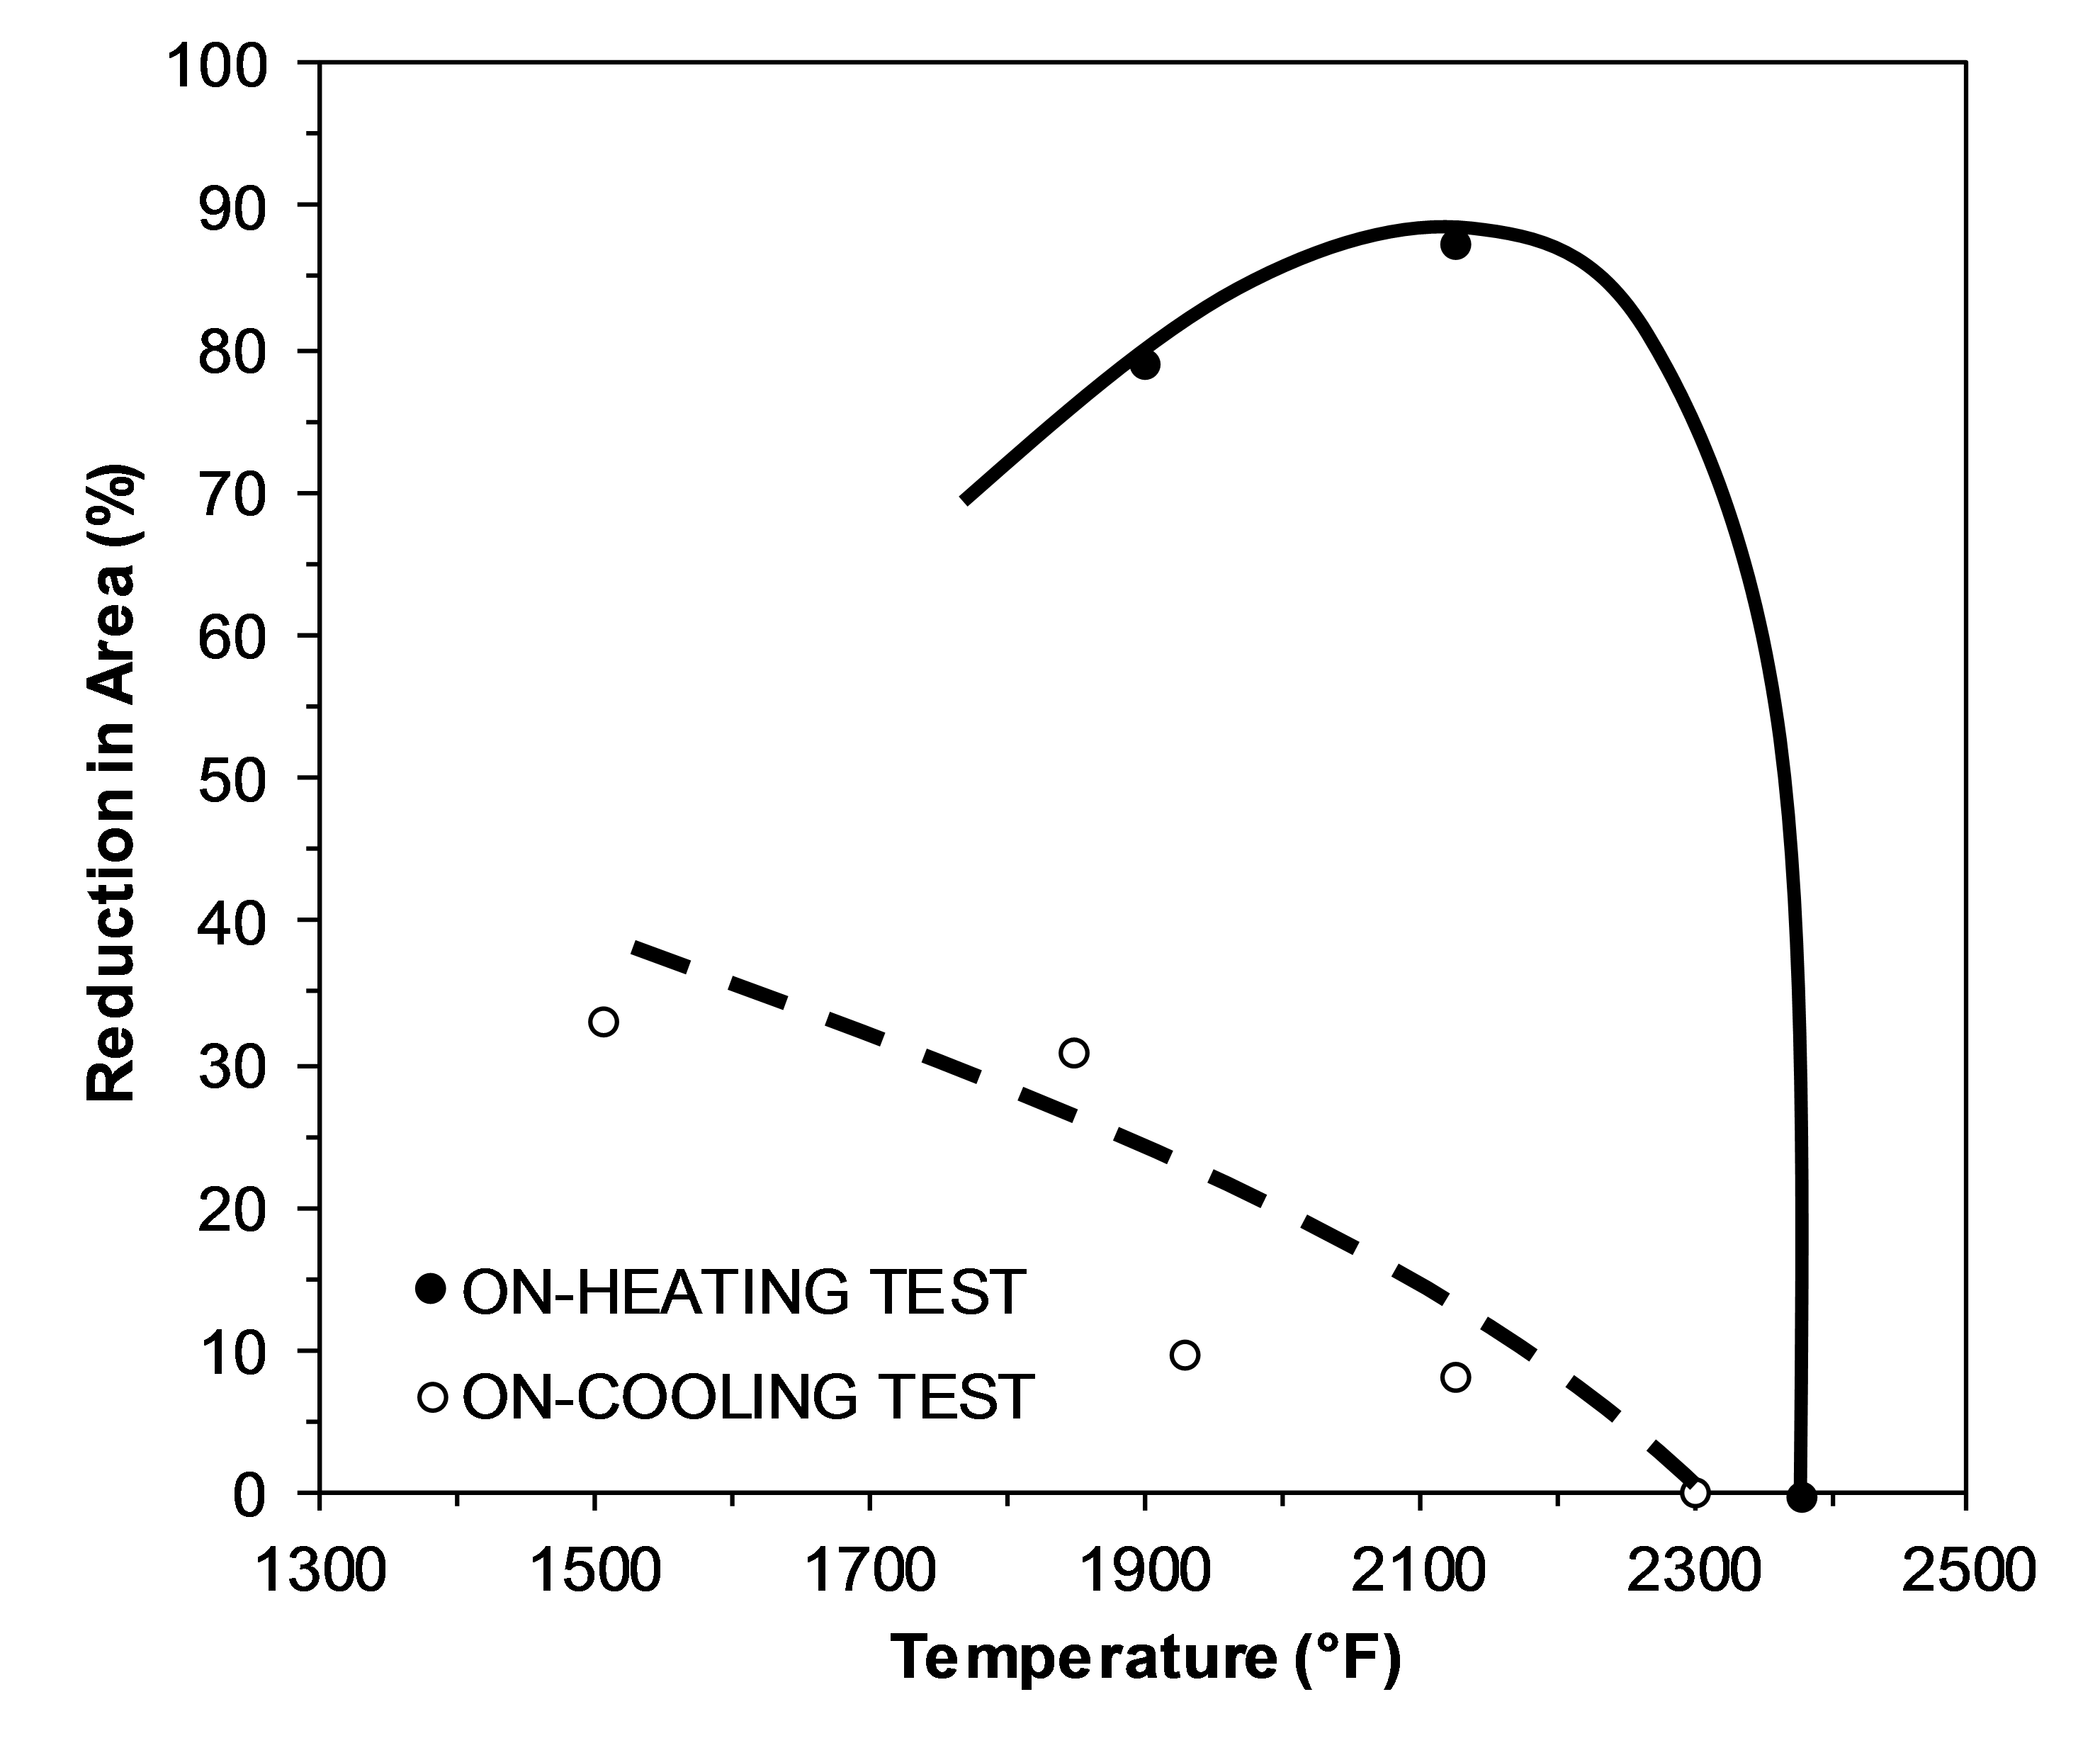
\includegraphics{figures/qiao-hot-ductility-800h-susceptible-r1.png}
    \caption{Hot ductility behavior of wrought modified 800H material exhibiting poor ductility recovery and classified as ``crack sensitive'' based on hot ductility and Varestraint testing. Adapted from \citet{qiao_weldability_1993}.}
    \label{fig:qiao-hot-ductility-800h-susceptible}
\end{figure}

\begin{figure}
    \centering
    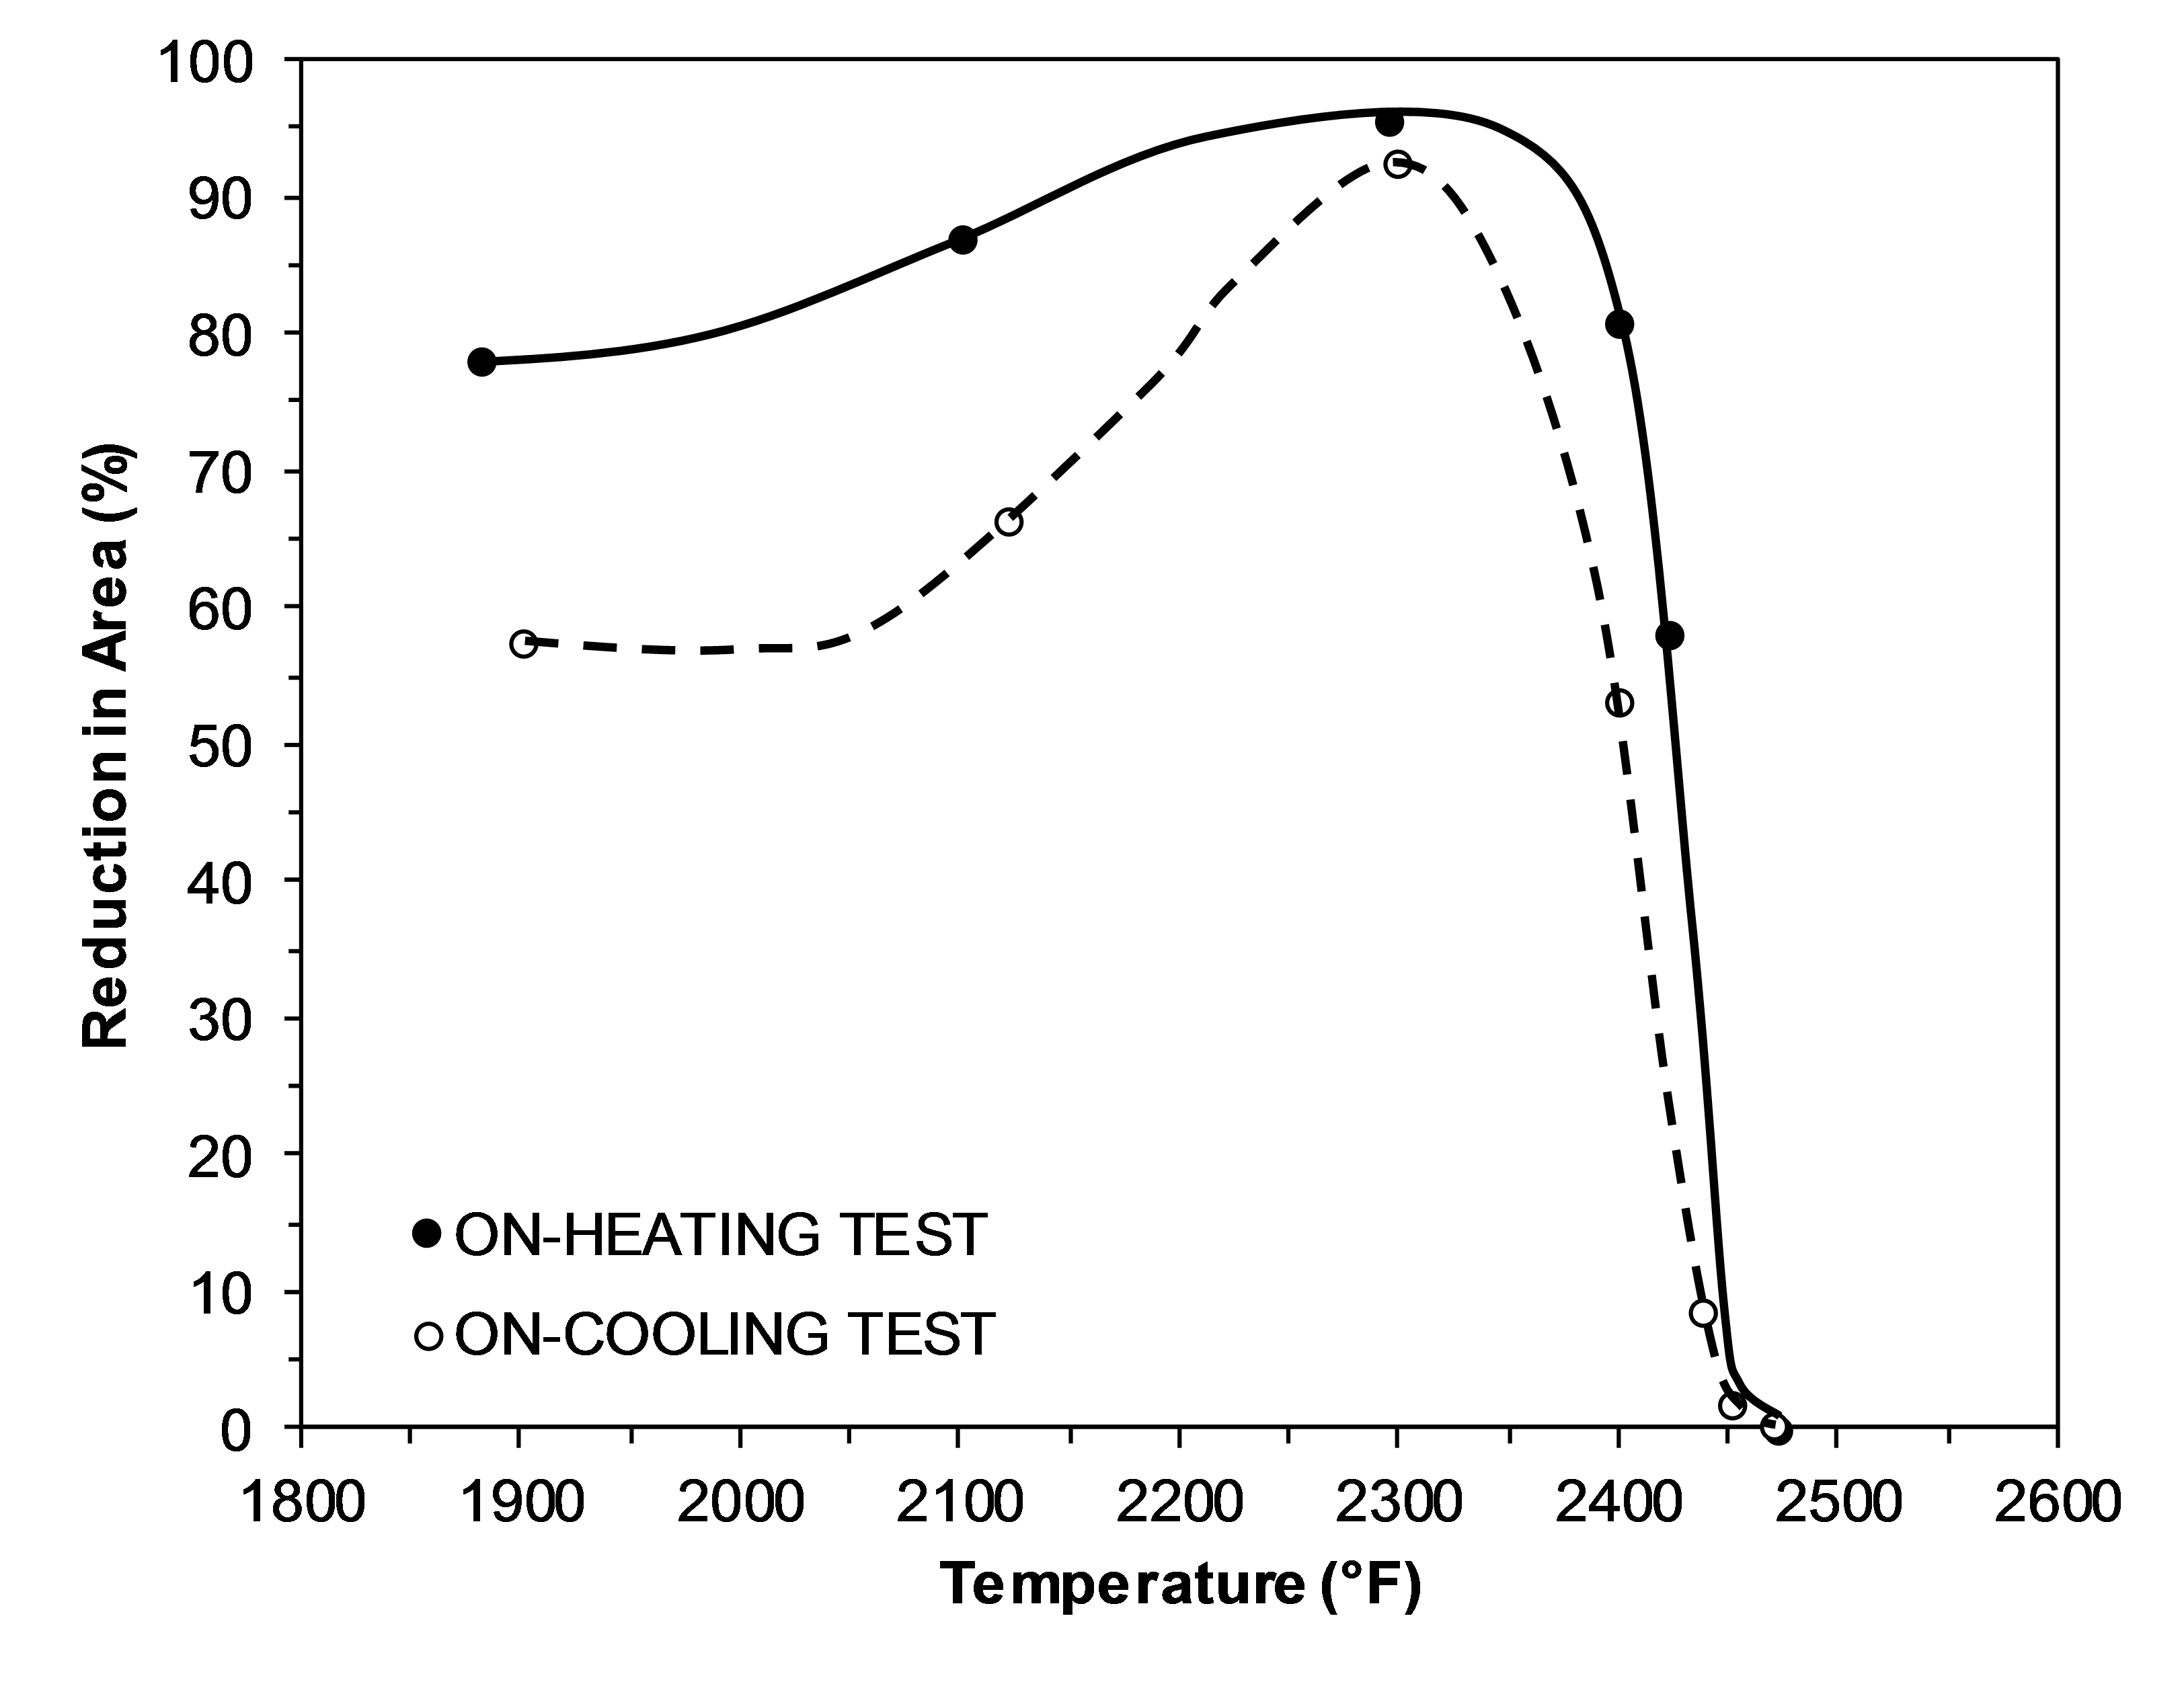
\includegraphics{figures/qiao-hot-ductility-ref-316-r1.png}
    \caption{Hot ductility behavior of 316 stainless steel exhibiting excellent ductility recovery with correspondingly low susceptibility to \gls{haz} liquation cracking. Adapted from \citet{qiao_weldability_1993}.}
    \label{fig:qiao-hot-ductility-316}
\end{figure}

\section{Microstructural Characterization}
\subsection{Characterization of As-Received Base Metals}
The typical as-received microstructures for the Cone~1 and Cone~5 materials, respectively, are shown in the optical micrographs in Figure~\ref{fig:c1-asreceived} and Figure~\ref{fig:c5-asreceived}.  Both Cone materials exhibited a cast, dendritic structure with a large dendrite size.  The 500X magnification micrographs in Figure~\ref{subfig:c1-asreceived-500X} and Figure~\ref{subfig:c5-asreceived-500X} show the presence of abundant fine intradendritic precipitates in the austenite matrix in addition to the larger phases along the interdendritic boundaries. The as-received Cone~1 and Cone~5 base metals were also examined in the \gls{sem} to perform \gls{eds} analyses of some of the constituents. \Gls{sem} micrographs and \gls{eds} results for typical Cone~1 and Cone~5 microstructures are presented in Figures \ref{fig:c1-ar-sem} and \ref{fig:c1-ar-eds} and Figures \ref{fig:c5-ar-sem} and \ref{fig:c5-ar-eds}, respectively. For Cone~1 material, Figure~\ref{fig:c1-ar-sem} shows both coarse interdendritic phases (e.g. ``A'' in Figure~\ref{subfig:c1-ar-sem-5kx}) and clusters of finer precipitates (``B'' in Figure~\ref{subfig:c1-ar-sem-5kx}). The \gls{eds} results in Figure~\ref{fig:c1-ar-eds}, corresponding to points ``A'' and ``B'' in Figure~\ref{subfig:c1-ar-sem-5kx}, show a high amount of niobium indicating that both regions consist of niobium carbides (NbC). It should be noted that in Figure~\ref{fig:c1-ar-eds} (and all subsequent \gls{eds} determinations), carbon has been excluded from the quantitative results because it is difficult to accurately assess carbon with \gls{eds}. These interdendritic NbC particles are apparent in the optical micrographs in Figures~\ref{fig:c1-asreceived} and \ref{fig:c5-asreceived} (e.g. as the larger ``salmon''-colored phases). The chromium, iron, and nickel contents reported for point ``B'' are considered to arise from beam interaction with the surrounding matrix, due to the small size of the analyzed particles. Similarly for the Cone~5 material, Figure~\ref{fig:c5-ar-sem} shows coarse interdendritic phases (``A'' in Figure~\ref{subfig:c5-ar-sem-5kx}) with finer phases present at the periphery (area ``B'' in Figure~\ref{subfig:c5-ar-sem-5kx}). Both ``A'' and ``B'' in Figure~\ref{subfig:c5-ar-sem-5kx} contain a high amount of niobium as shown in Figure~\ref{fig:c5-ar-eds}, corresponding to NbC. The compositions of the very fine (<< \SI{1}{\micro\meter}) intradendritic precipitates, visible in both Cone~1 and Cone~5 in Figure~\ref{subfig:c1-ar-sem-1kx} and Figure~\ref{subfig:c5-ar-sem-1kx} respectively, were not determined because these precipitates are too small to be analyzed with \gls{eds}. 

It should be noted that in service-exposed 20Cr-32Ni-Nb material, the formation of a secondary phase rich in nickel, niobium, and silicon (``Ni-Nb silicide'') around the NbC carbides often occurs as reported by a number of authors \cite{shi_microstructure_2008,hoffman_high_2000-1,knowles_service_2004,patchett_welding_1998}. The formation of Cr-rich M23C6 carbides along the interdendritic boundaries has also been reported after service exposure \cite{shi_microstructure_2008,patchett_welding_1998}. However, the presence of Cr-rich M23C6 carbides or Ni-Nb-Si-rich phases around the NbC carbides was not observed in either the Cone~1 or Cone~5 materials despite the fact that they were reported to be in service-exposed condition with ~15 y of exposure at 1575\textdegree{}F. \citet{hoffman_high_2000-1} observed differences in the extent of Ni-Nb-Si-rich phase formation (which he identified as G-phase) between statically cast tees and centrifugally cast cones with different compositions, with the cone material having a lesser (unspecified) extent of silicide formation. Compared to the service conditions and materials reported by other workers \cite{hoffman_high_2000-1,patchett_welding_1998,knowles_service_2004,shi_microstructure_2008}, in some cases the Cone~1 and Cone~5 materials (this study) reportedly have longer service exposure time or higher service temperature. In a 25Cr-32Ni-2Nb alloy, higher temperatures (~1800\textdegree{}F) have been associated with reduced stability of G-phase \cite{de_almeida_soares_niobium_1992}. However, this temperature is well above the reported service temperature of the two materials examined in thus study, making it unlikely that the reported service temperature of 1575\textdegree{}F for Cone~1 and Cone~5 is responsible for the disparity between observation of G-phase as reported in the literature and the lack of G-phase in the current materials. 

%The lack of published time-temperature precipitation (TTP) data for the 20Cr-32Ni-Nb alloy (cite Patchet??) makes it difficult to ascertain if this is the case.}

%Ni-Nb-Si phases, cite Shi, Hoffman 2000, KNowles 2004, Patchett 1998, Shibasaki

%Under the beam conditions used for the current analyses, the interaction volume that is sampled by a single ``spot'' \gls{eds} analysis is [volume].

%Figure X and Figure Y present higher magnification SEM micrographs of the typical Cone~1 microstructure along with \gls{eds} results.

\begin{figure}
    \centering
    \subfloat[100X]{\label{subfig:c1-asreceived-100X}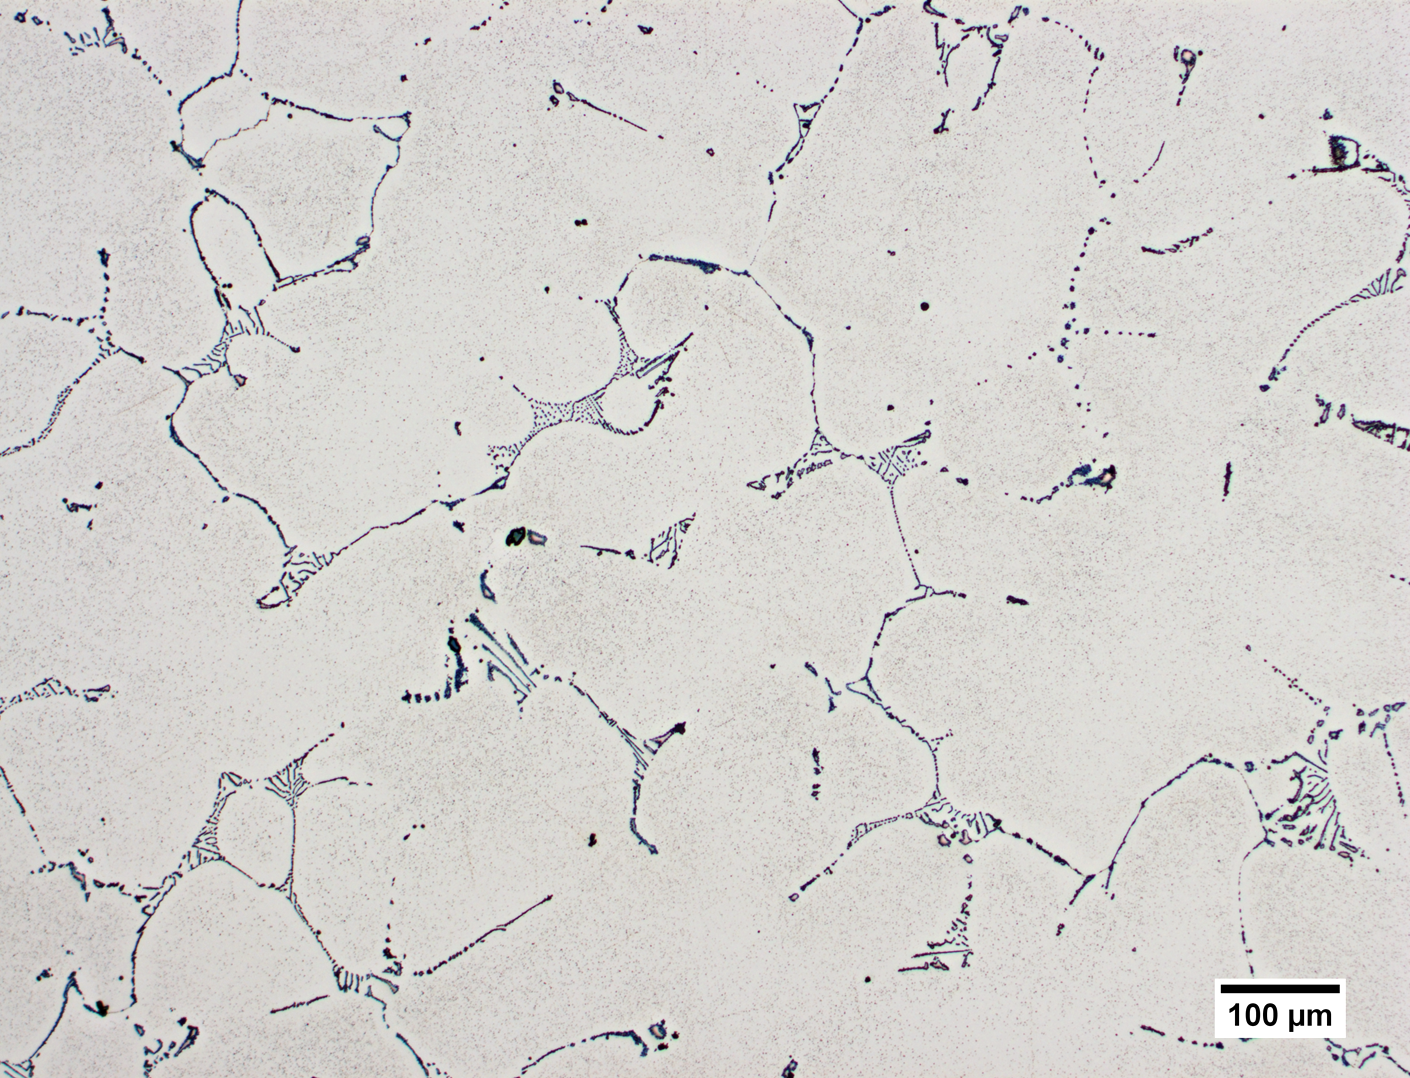
\includegraphics[width=4.7in]{figures/metallography/c1-ar-100X}} \\
    \subfloat[500X]{\label{subfig:c1-asreceived-500X}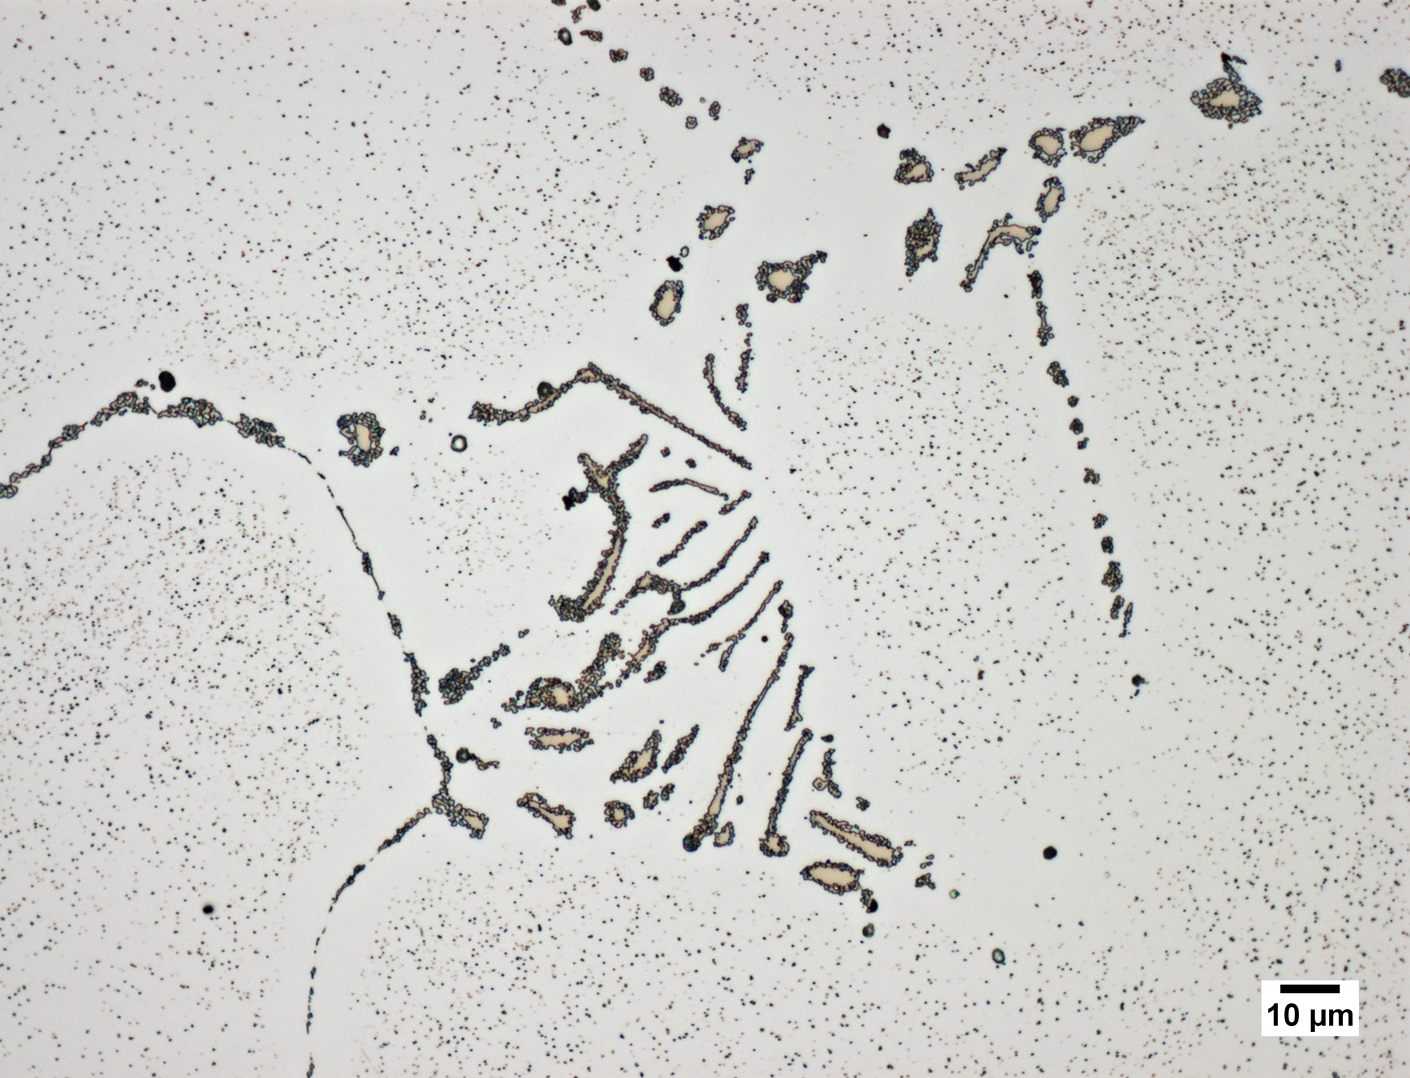
\includegraphics[width=4.7in]{figures/metallography/c1-ar-500X}}
    \caption[Optical micrographs showing the typical as-received microstructure of Cone~1 Material.]{Optical micrographs showing the typical as-received microstructure of Cone~1 material utilized for hot ductility testing, (A) 100X and (B) 500X.  Etch: electrolytic 10\% oxalic acid.}
    \label{fig:c1-asreceived}
\end{figure}

\begin{figure}
    \centering
    \subfloat[100X]{\label{subfig:c5-asreceived-100X}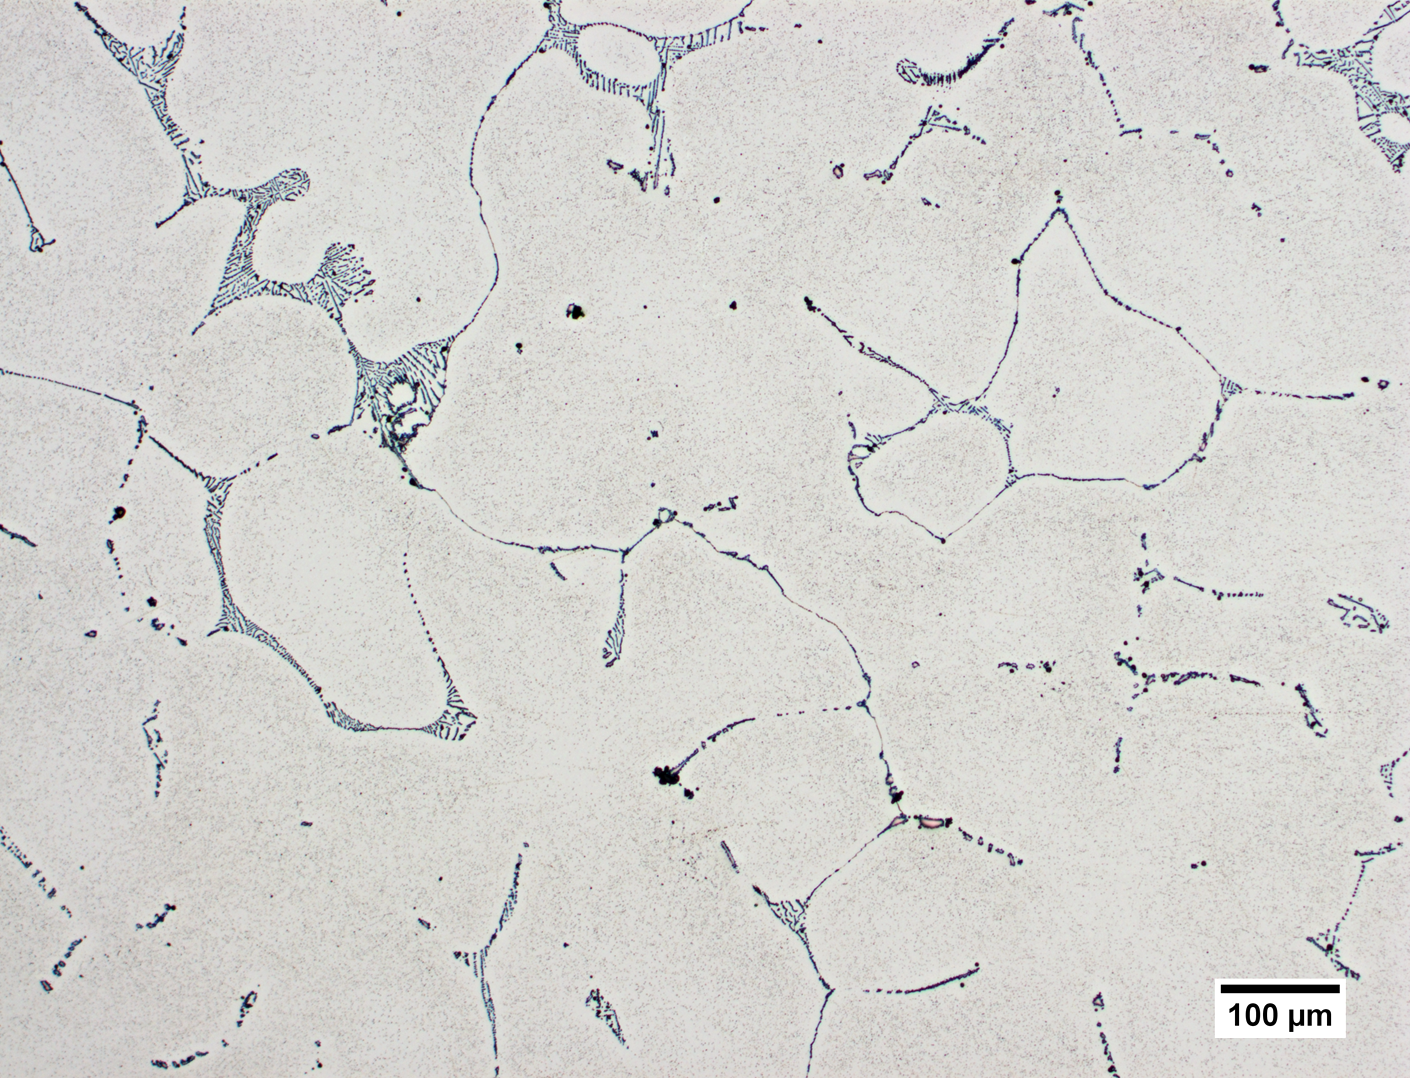
\includegraphics[width=4.7in]{figures/metallography/c5-ar-100X}} \\
    \subfloat[500X]{\label{subfig:c5-asreceived-500X}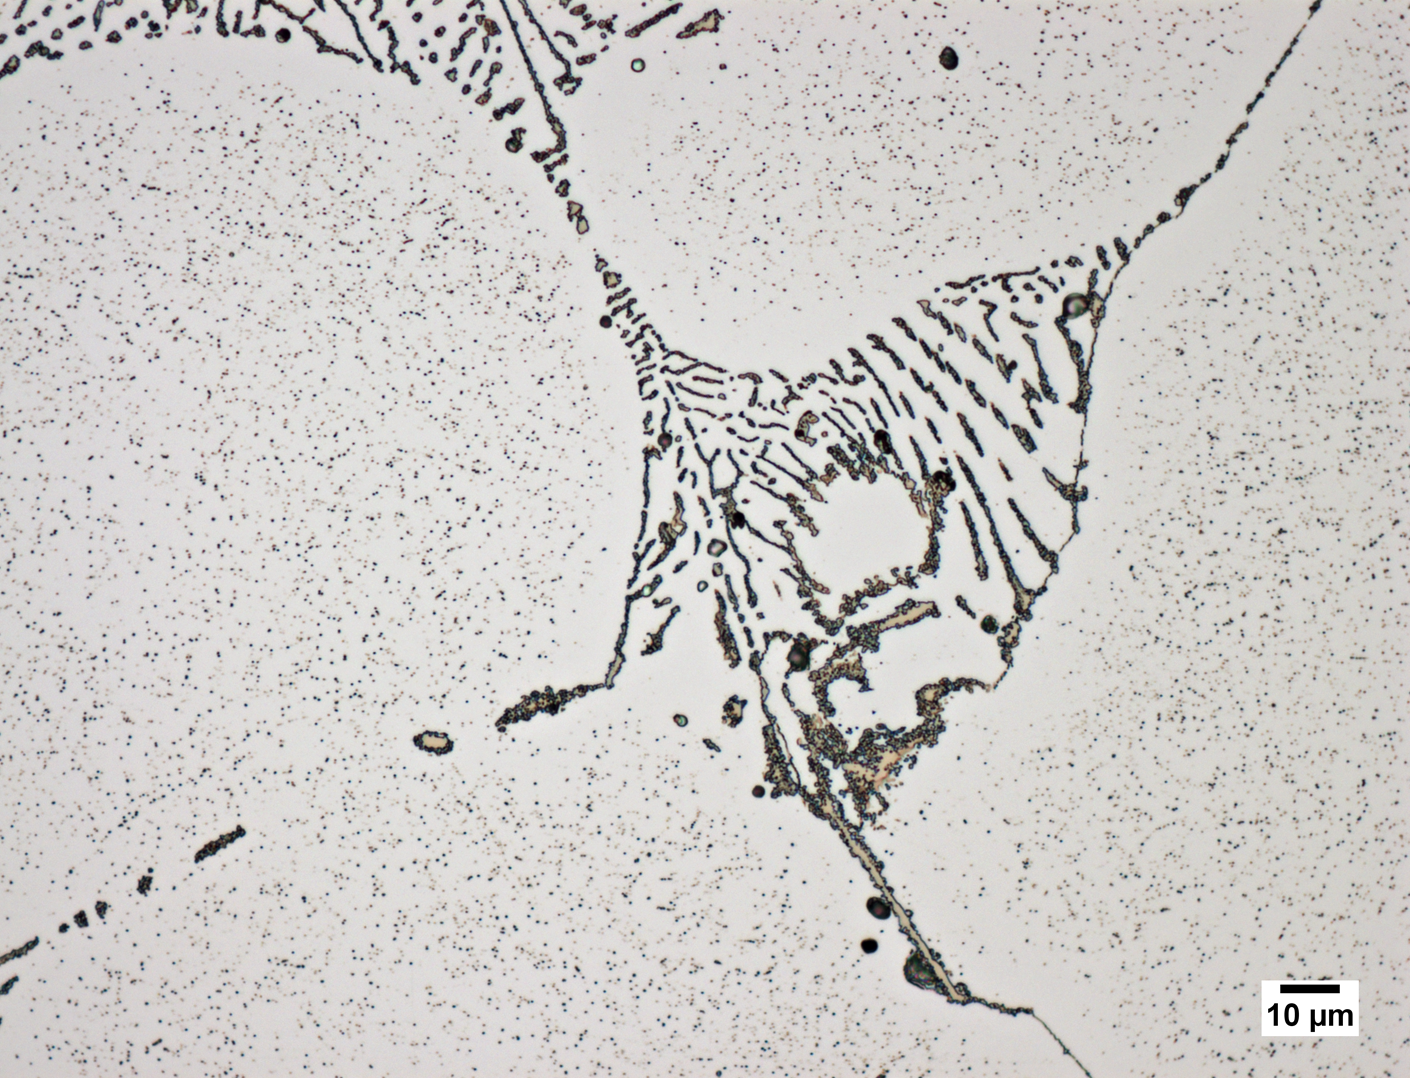
\includegraphics[width=4.7in]{figures/metallography/c5-ar-500X}}
    \caption[Optical micrographs showing the typical as-received microstructure of Cone~5 Material.]{Optical micrographs showing the typical as-received microstructure of Cone~5 material utilized for hot ductility testing, (A) 100X and (B) 500X.  Etch: electrolytic 10\% oxalic acid.}
    \label{fig:c5-asreceived}
\end{figure}

%C1 as-received SEM and EDS
\begin{figure}
    \centering
    \subfloat[1000X]{\label{subfig:c1-ar-sem-1kx}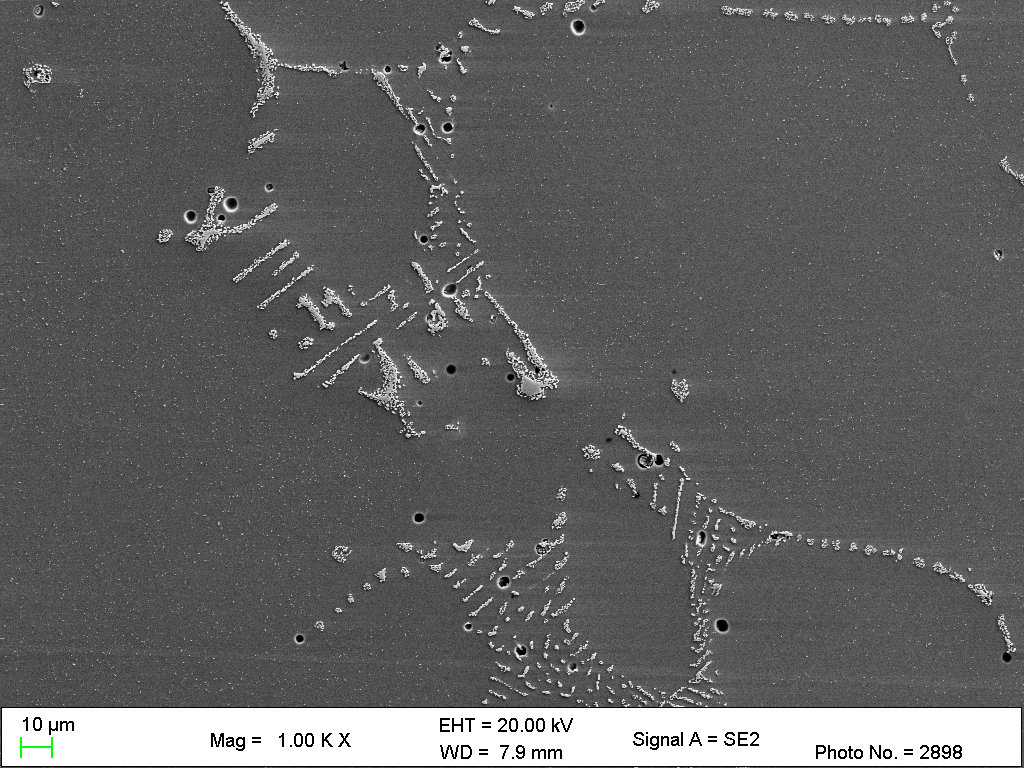
\includegraphics[width=4.7in]{figures/metallography/c1-ar-sem-1kx-L3-08.png}} \\
    \subfloat[5000X]{\label{subfig:c1-ar-sem-5kx}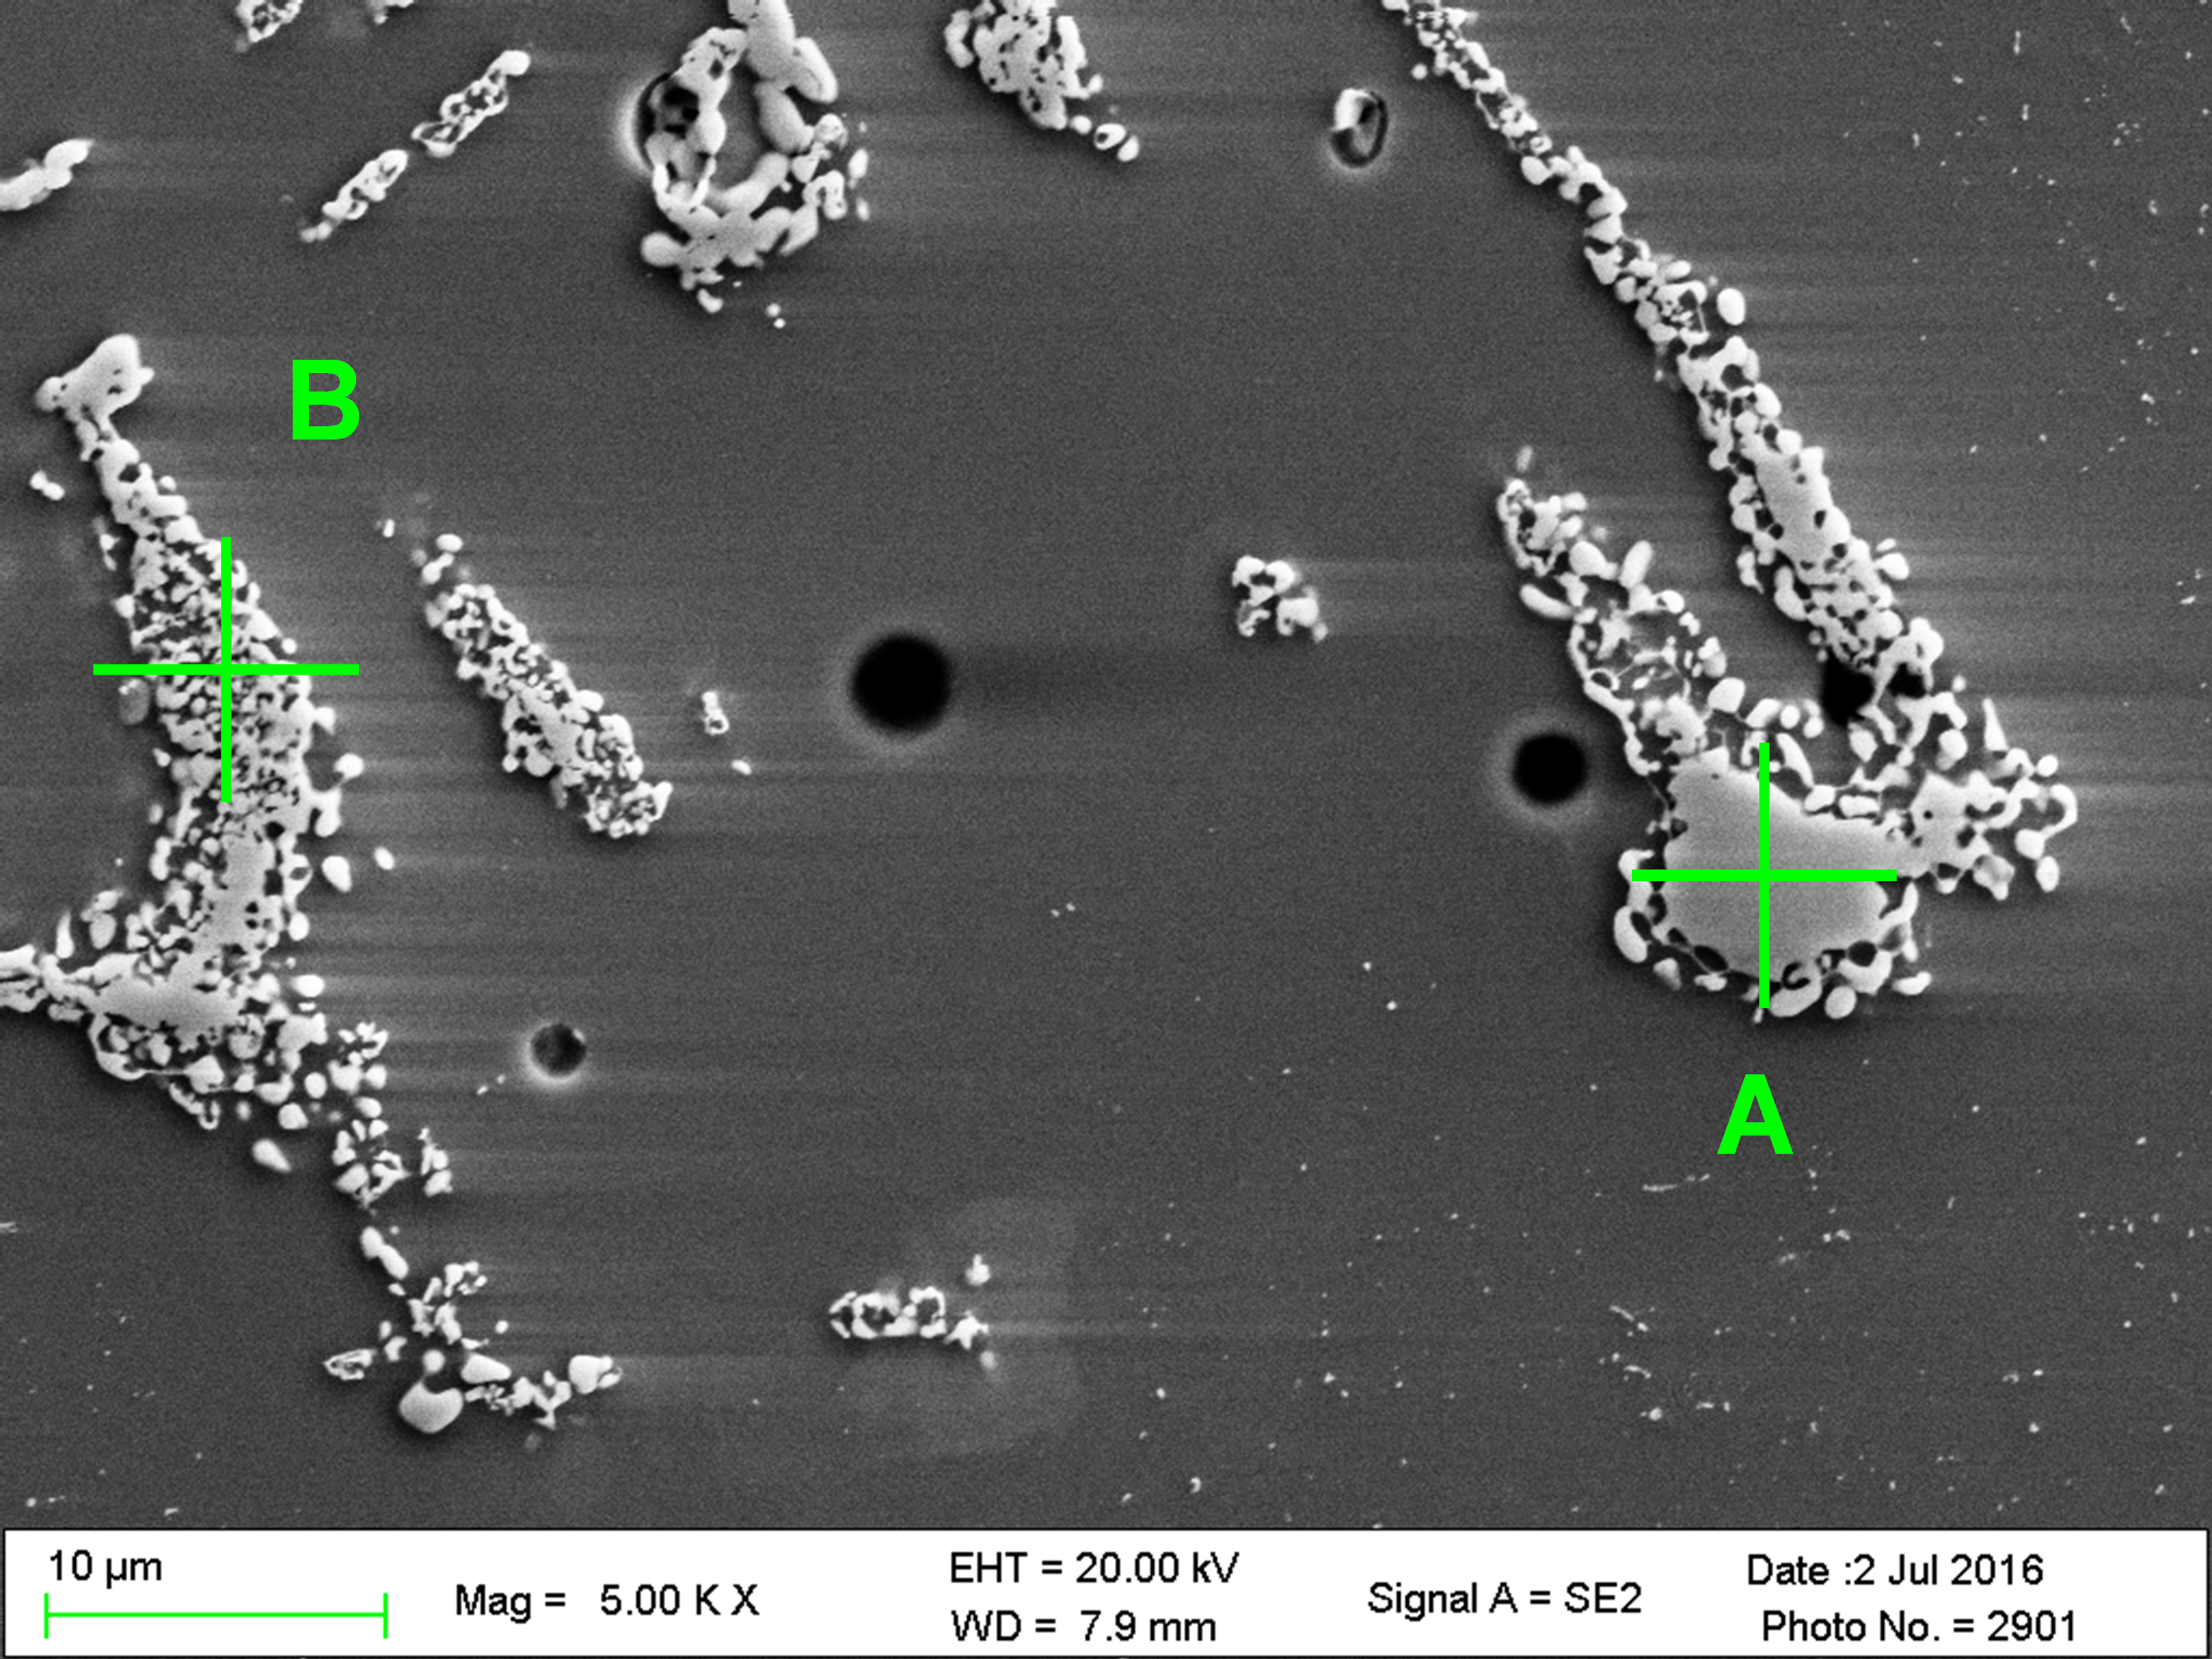
\includegraphics[width=4.7in]{figures/metallography/c1-ar-sem-5kx-L3-11.png}}
    \caption[\Gls{sem} micrographs showing typical intradendritic and interdendritic phases present in as-received Cone~1 material.]{\Gls{sem} micrographs showing typical intradendritic and interdendritic phases present in Cone~1 material utilized for hot ductility testing. \Gls{eds} spot analysis results for labeled locations ``A'' and ``B'' are given in Figure~\ref{fig:c1-ar-eds}. Etch: electrolytic 10\% oxalic acid.}
    \label{fig:c1-ar-sem}
\end{figure}

\begin{figure}
    \centering
    \subfloat[Spot Analysis ``A'']{\label{subfig:c1-ar-eds-a}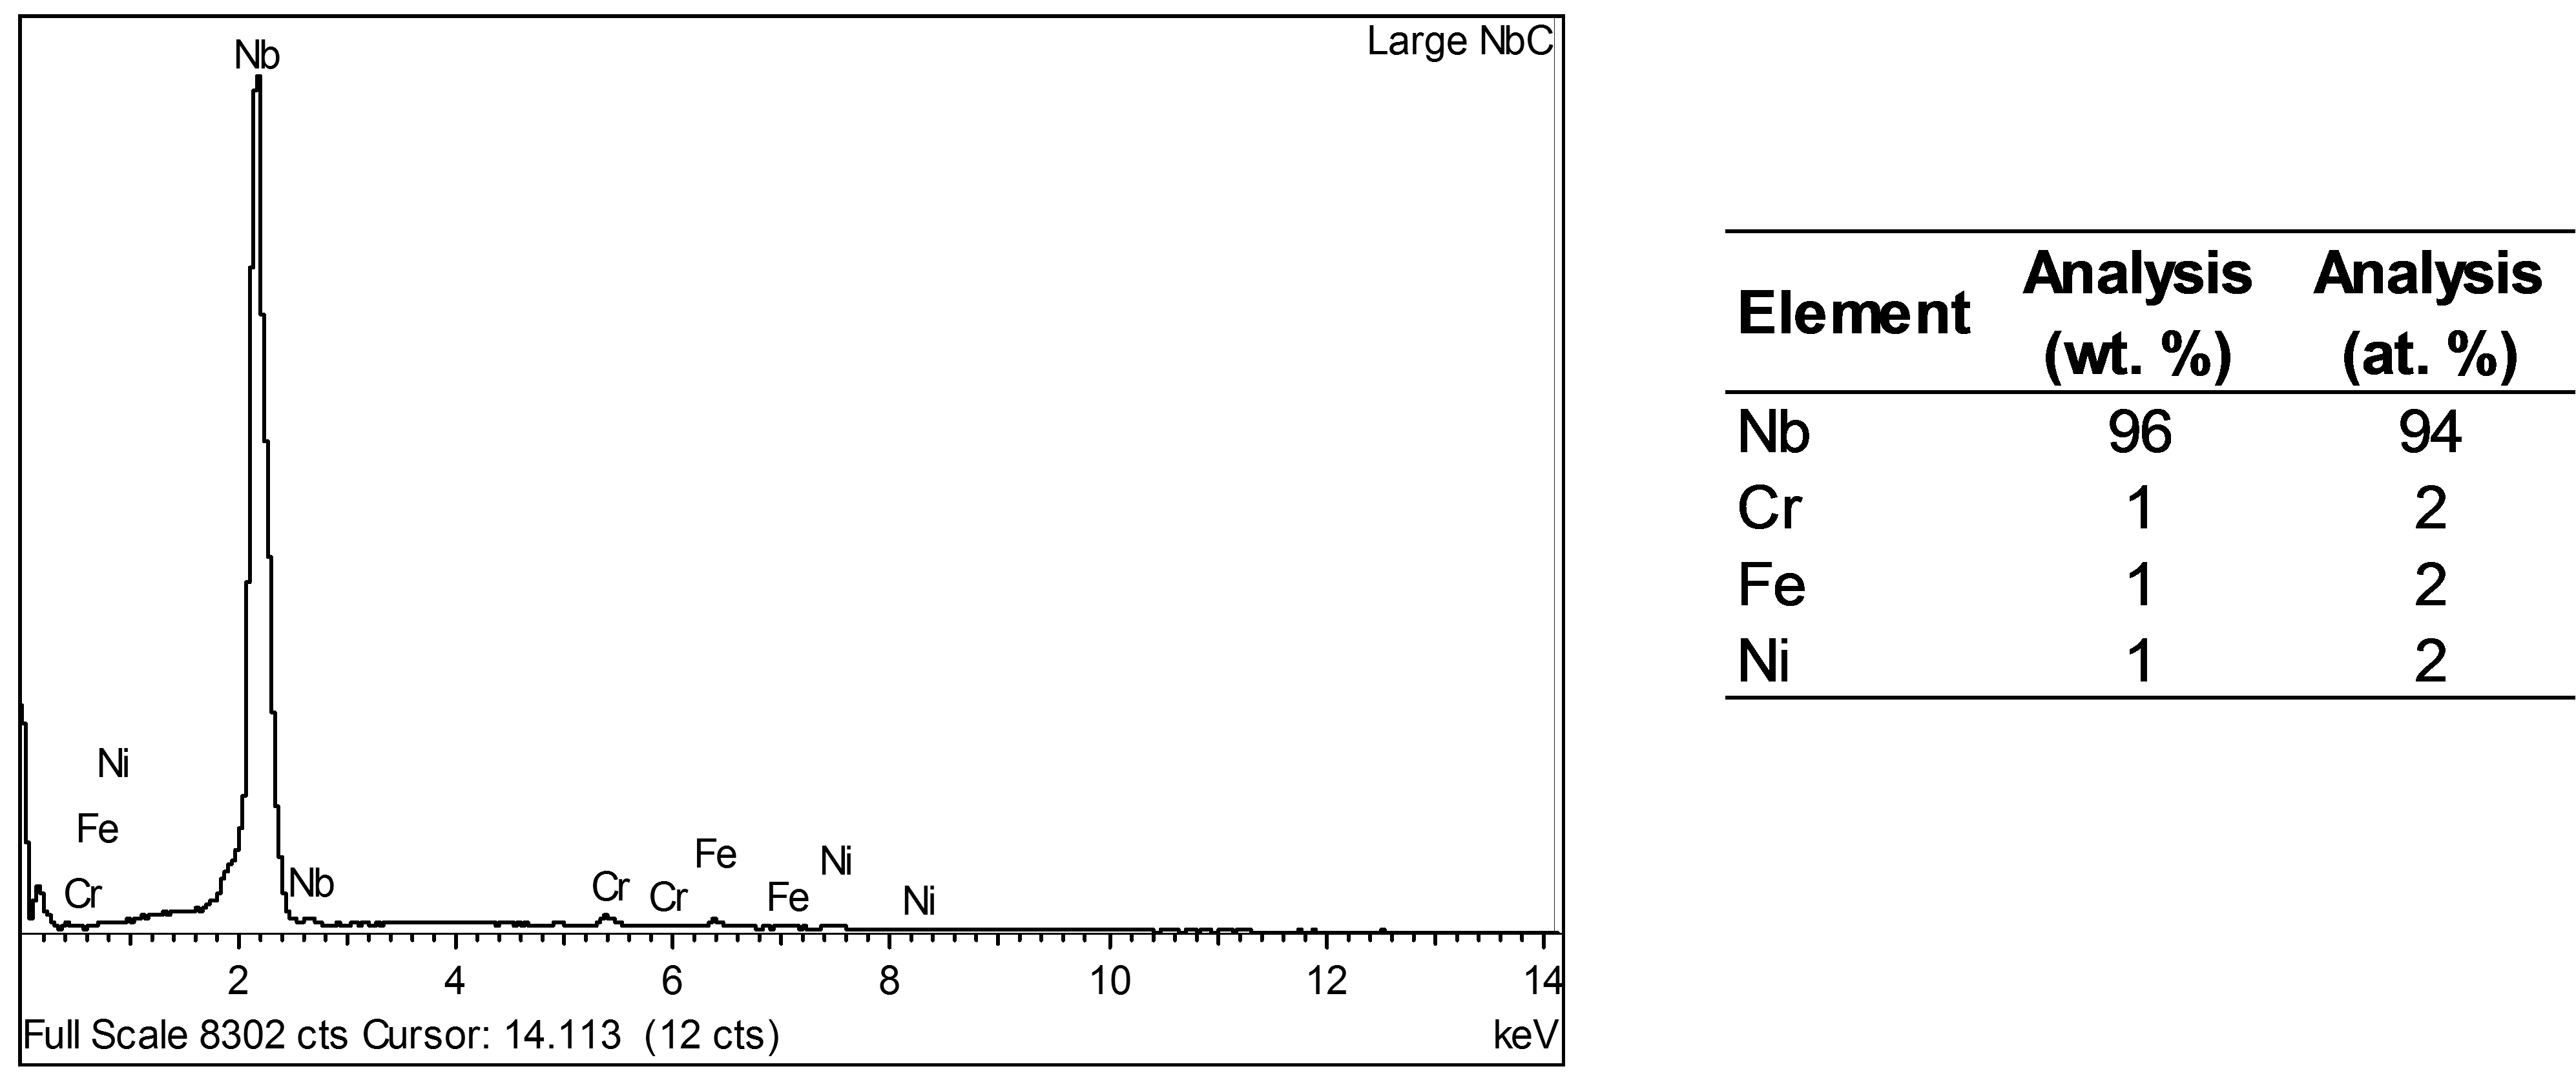
\includegraphics[width=\textwidth]{figures/metallography/c1-ar-eds-table-L3-A.png}} \\
    \subfloat[Spot Analysis ``B'']{\label{subfig:c1-ar-eds-b}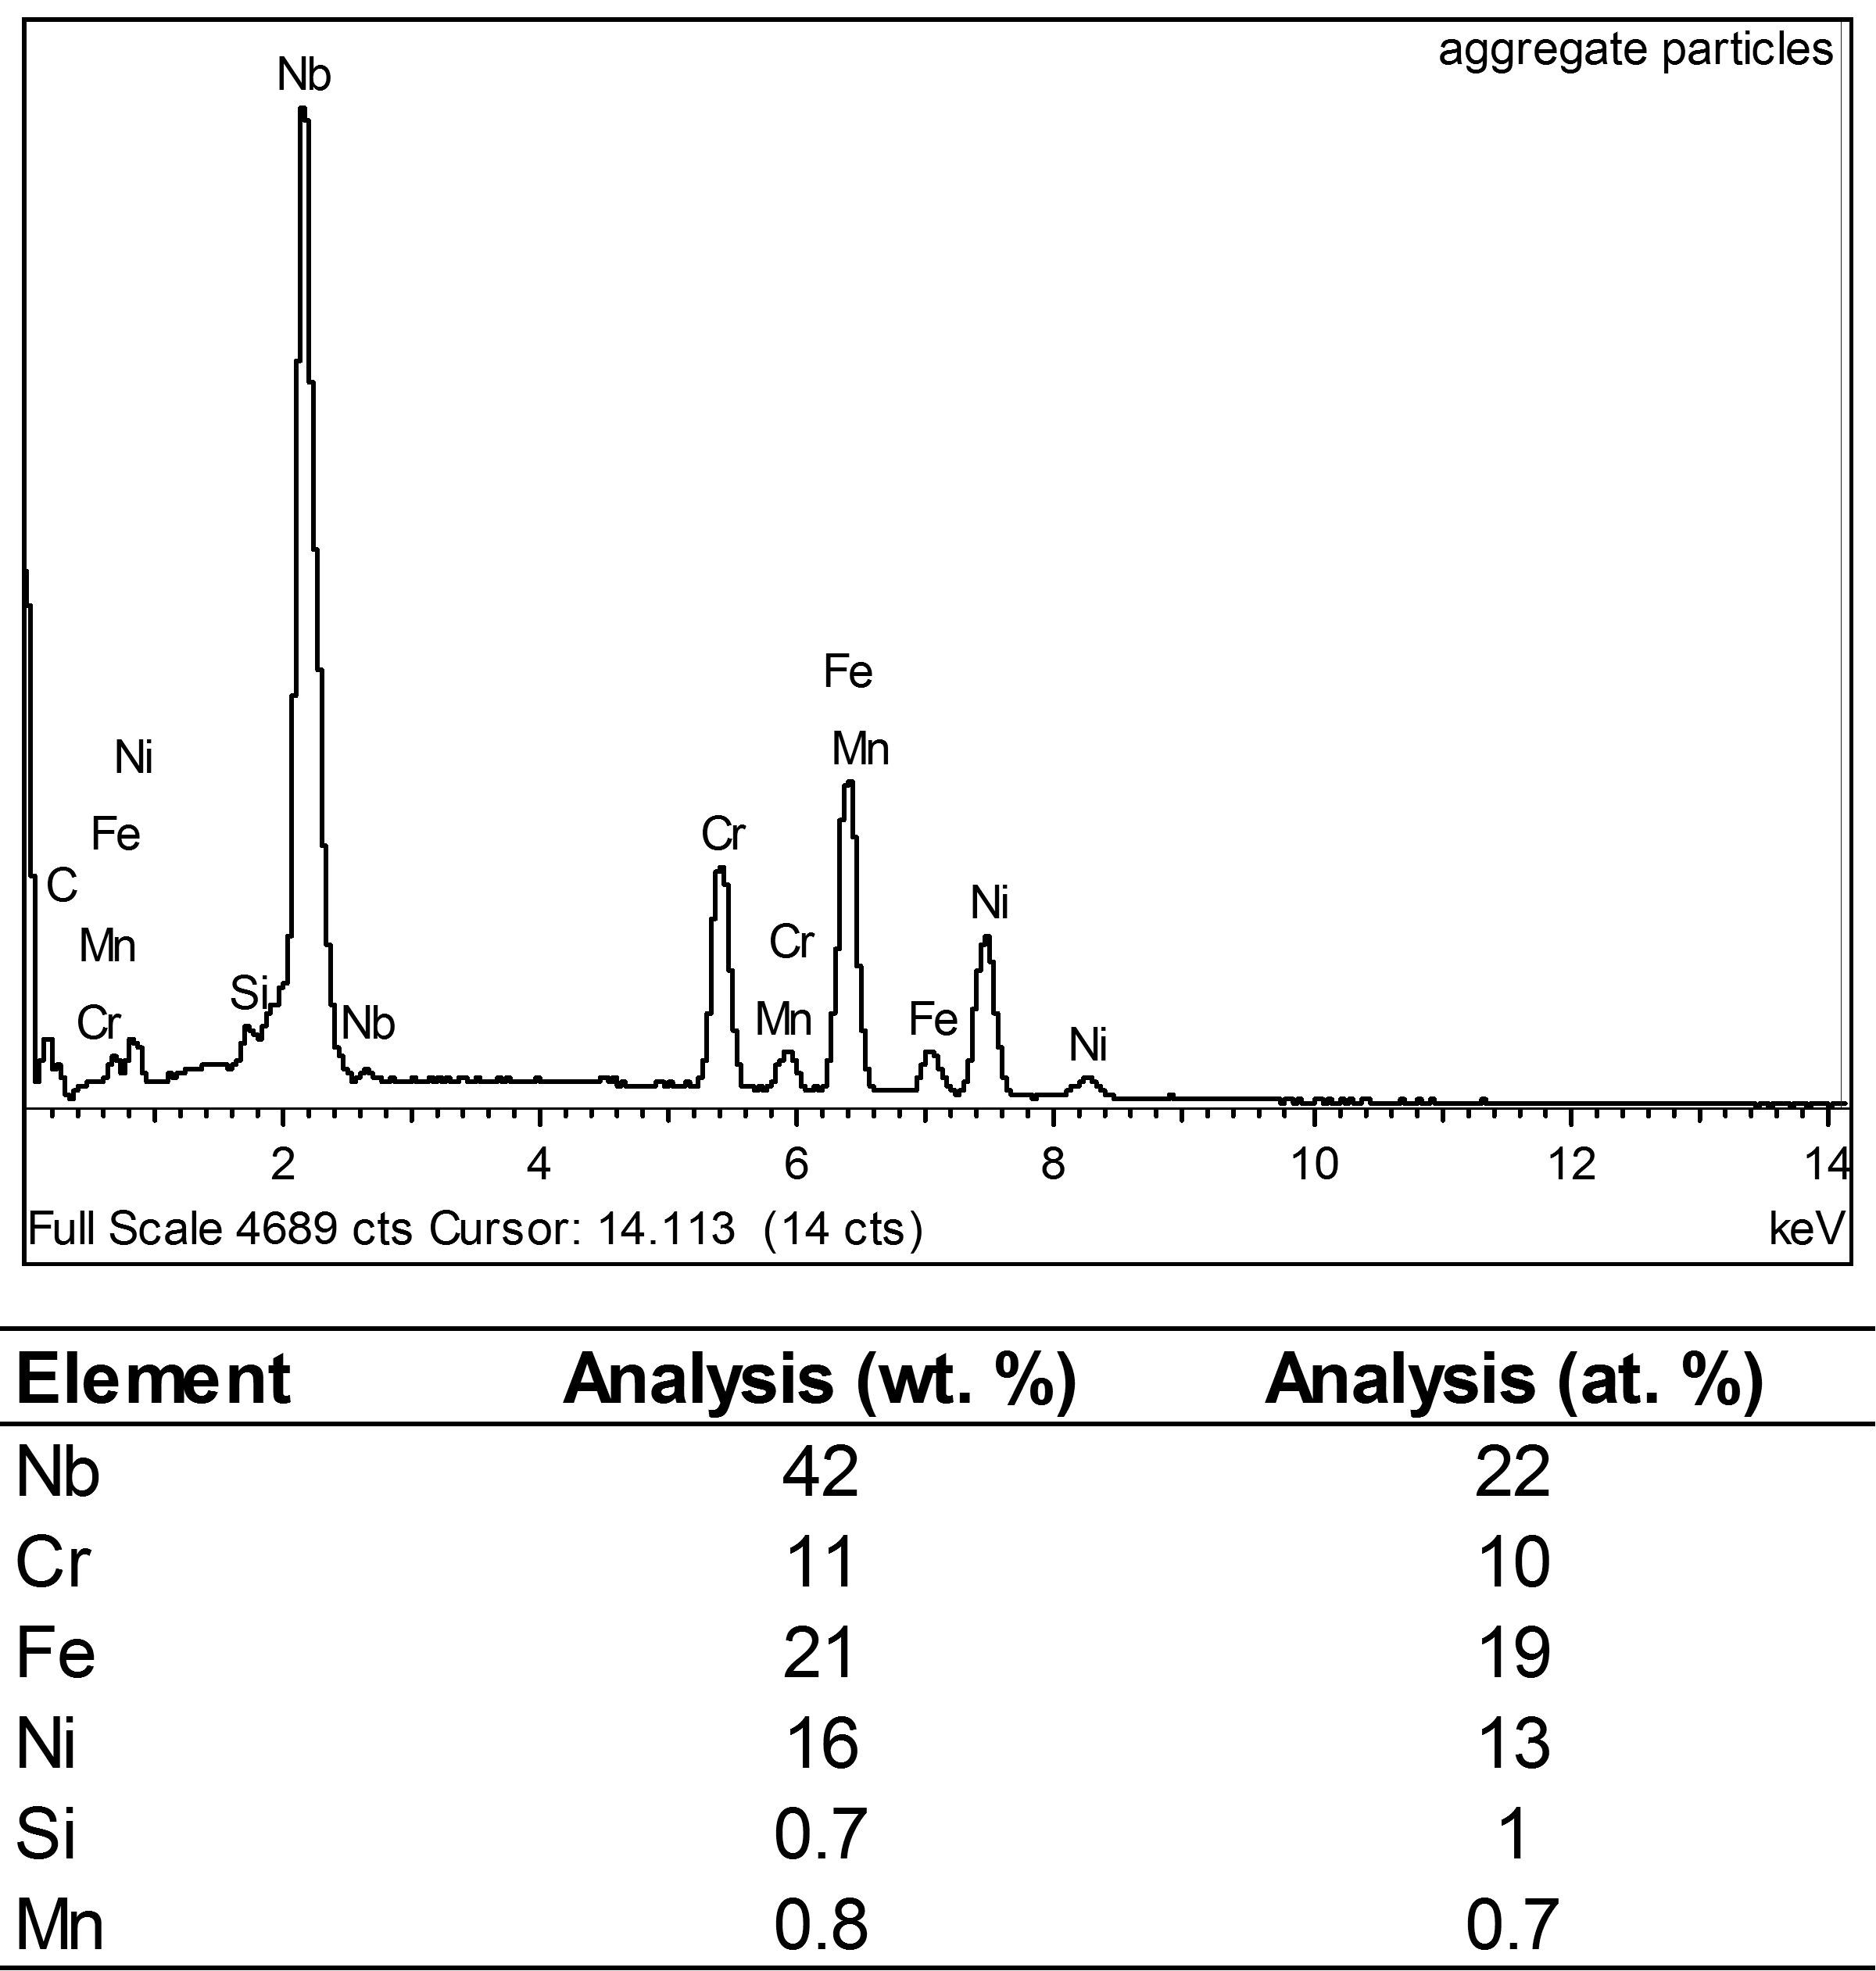
\includegraphics[width=\textwidth]{figures/metallography/c1-ar-eds-table-L3-B}}
    \caption[]{\Gls{eds} spot analysis results for locations ``A'' and ``B'' identified in Figure~\ref{subfig:c1-ar-sem-5kx} for as-received Cone~1 material.}
    \label{fig:c1-ar-eds}
\end{figure}

%C5 as-received SEM and EDS
\begin{figure}
    \centering
    \subfloat[1000X]{\label{subfig:c5-ar-sem-1kx}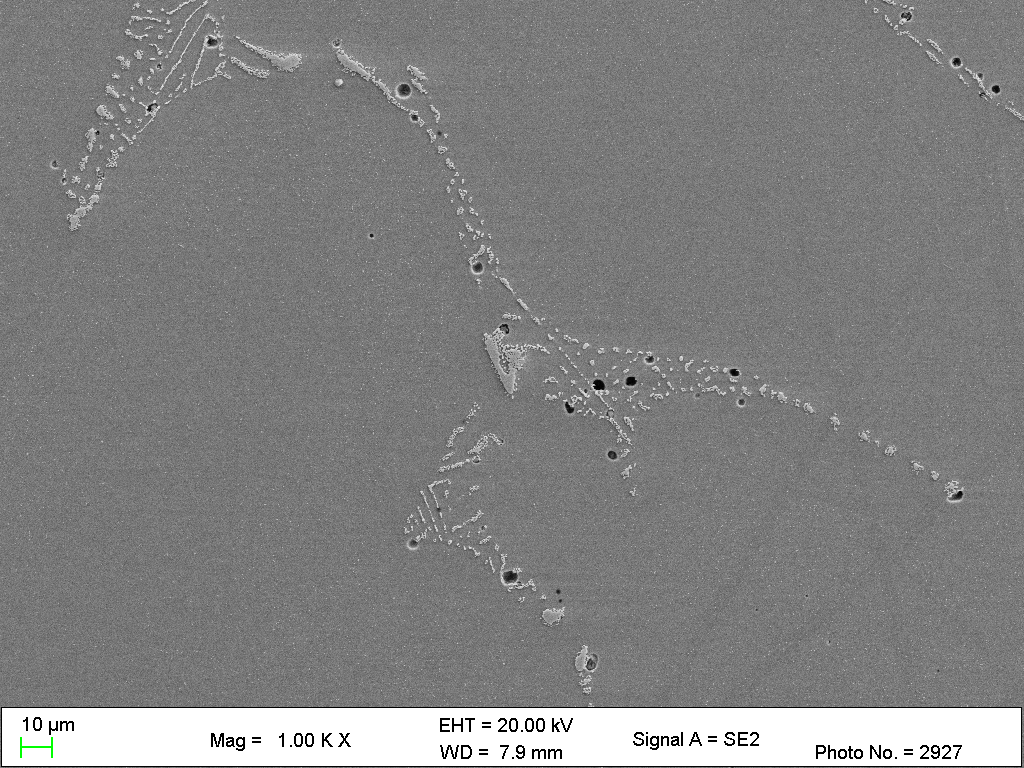
\includegraphics[width=4.7in]{figures/metallography/c5-ar-sem-1kx-L1-10.png}} \\
    \subfloat[5000X]{\label{subfig:c5-ar-sem-5kx}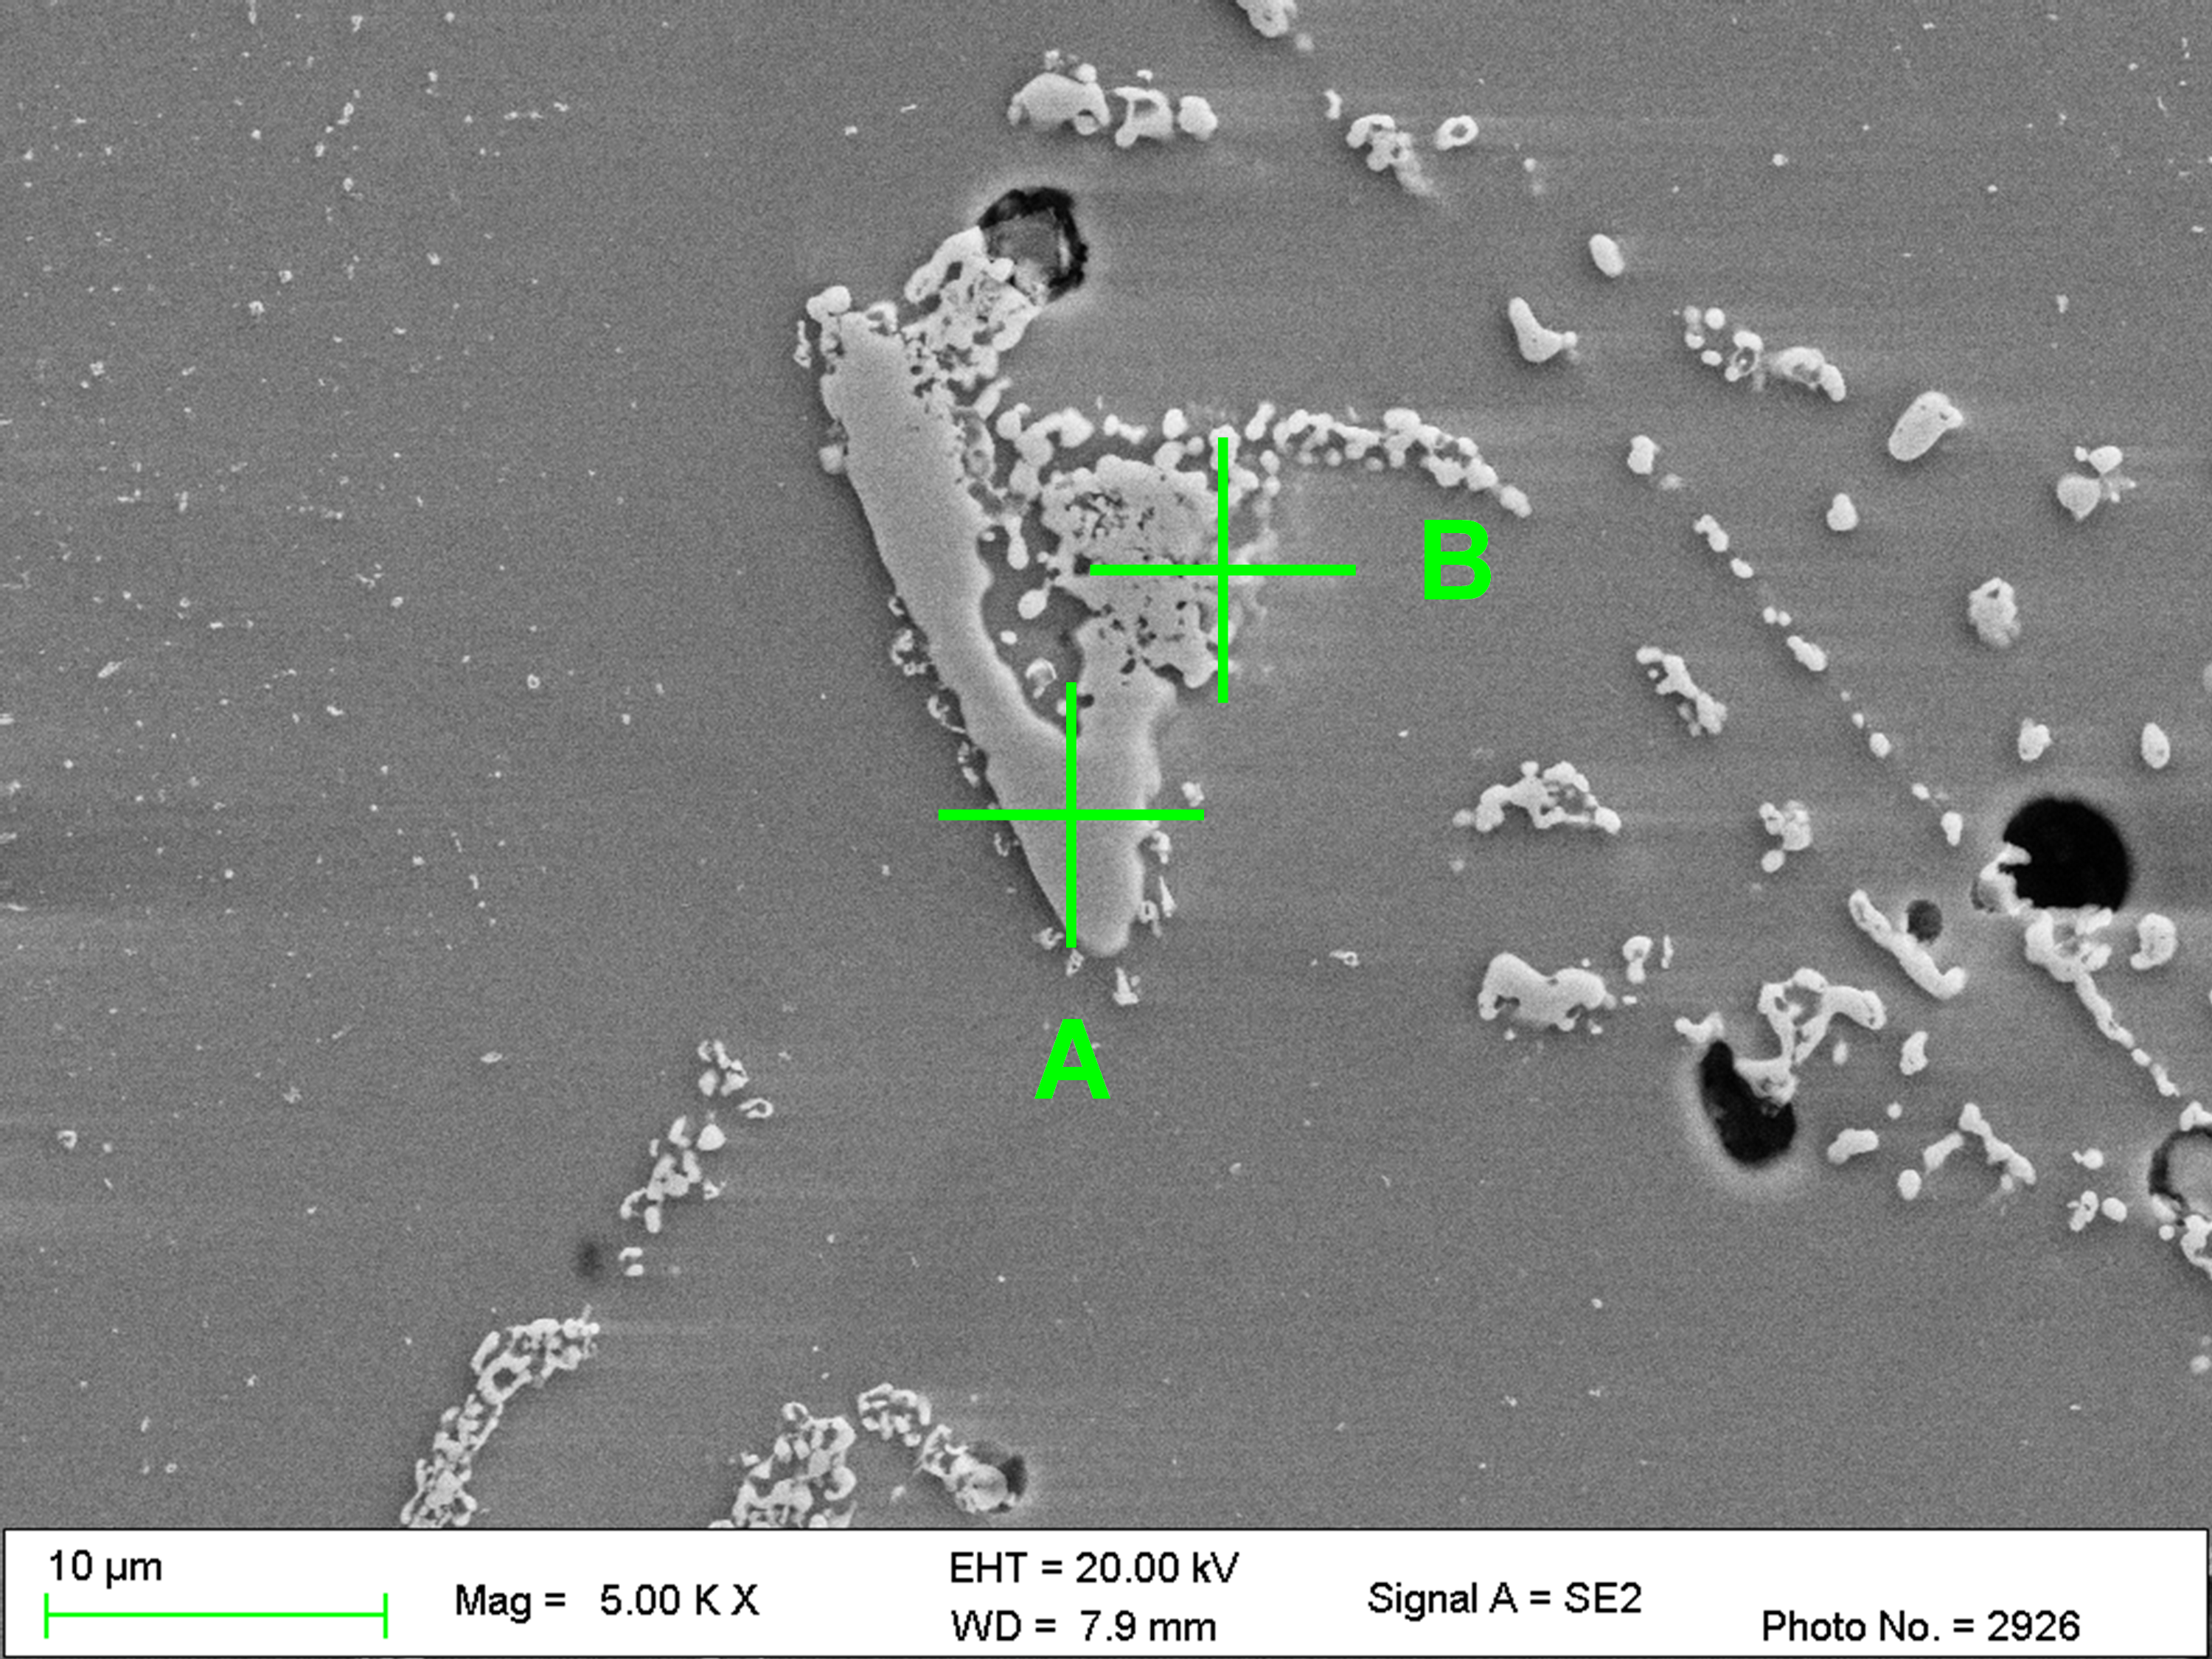
\includegraphics[width=4.7in]{figures/metallography/c5-ar-sem-5kx-L1-09.png}}
    \caption[\Gls{sem} micrographs showing typical intradendritic and interdendritic phases present in as-received Cone~5 material.]{\Gls{sem} micrographs showing typical intradendritic and interdendritic phases present in Cone~5 material utilized for hot ductility testing. \Gls{eds} analyses for labeled points ``A'' and ``B'' are given in Figure~\ref{fig:c5-ar-eds}. Etch: electrolytic 10\% oxalic acid.}
    \label{fig:c5-ar-sem}
\end{figure}

\begin{figure}
    \centering
    \subfloat[Spot Analysis ``A'']{\label{subfig:c5-ar-eds-a}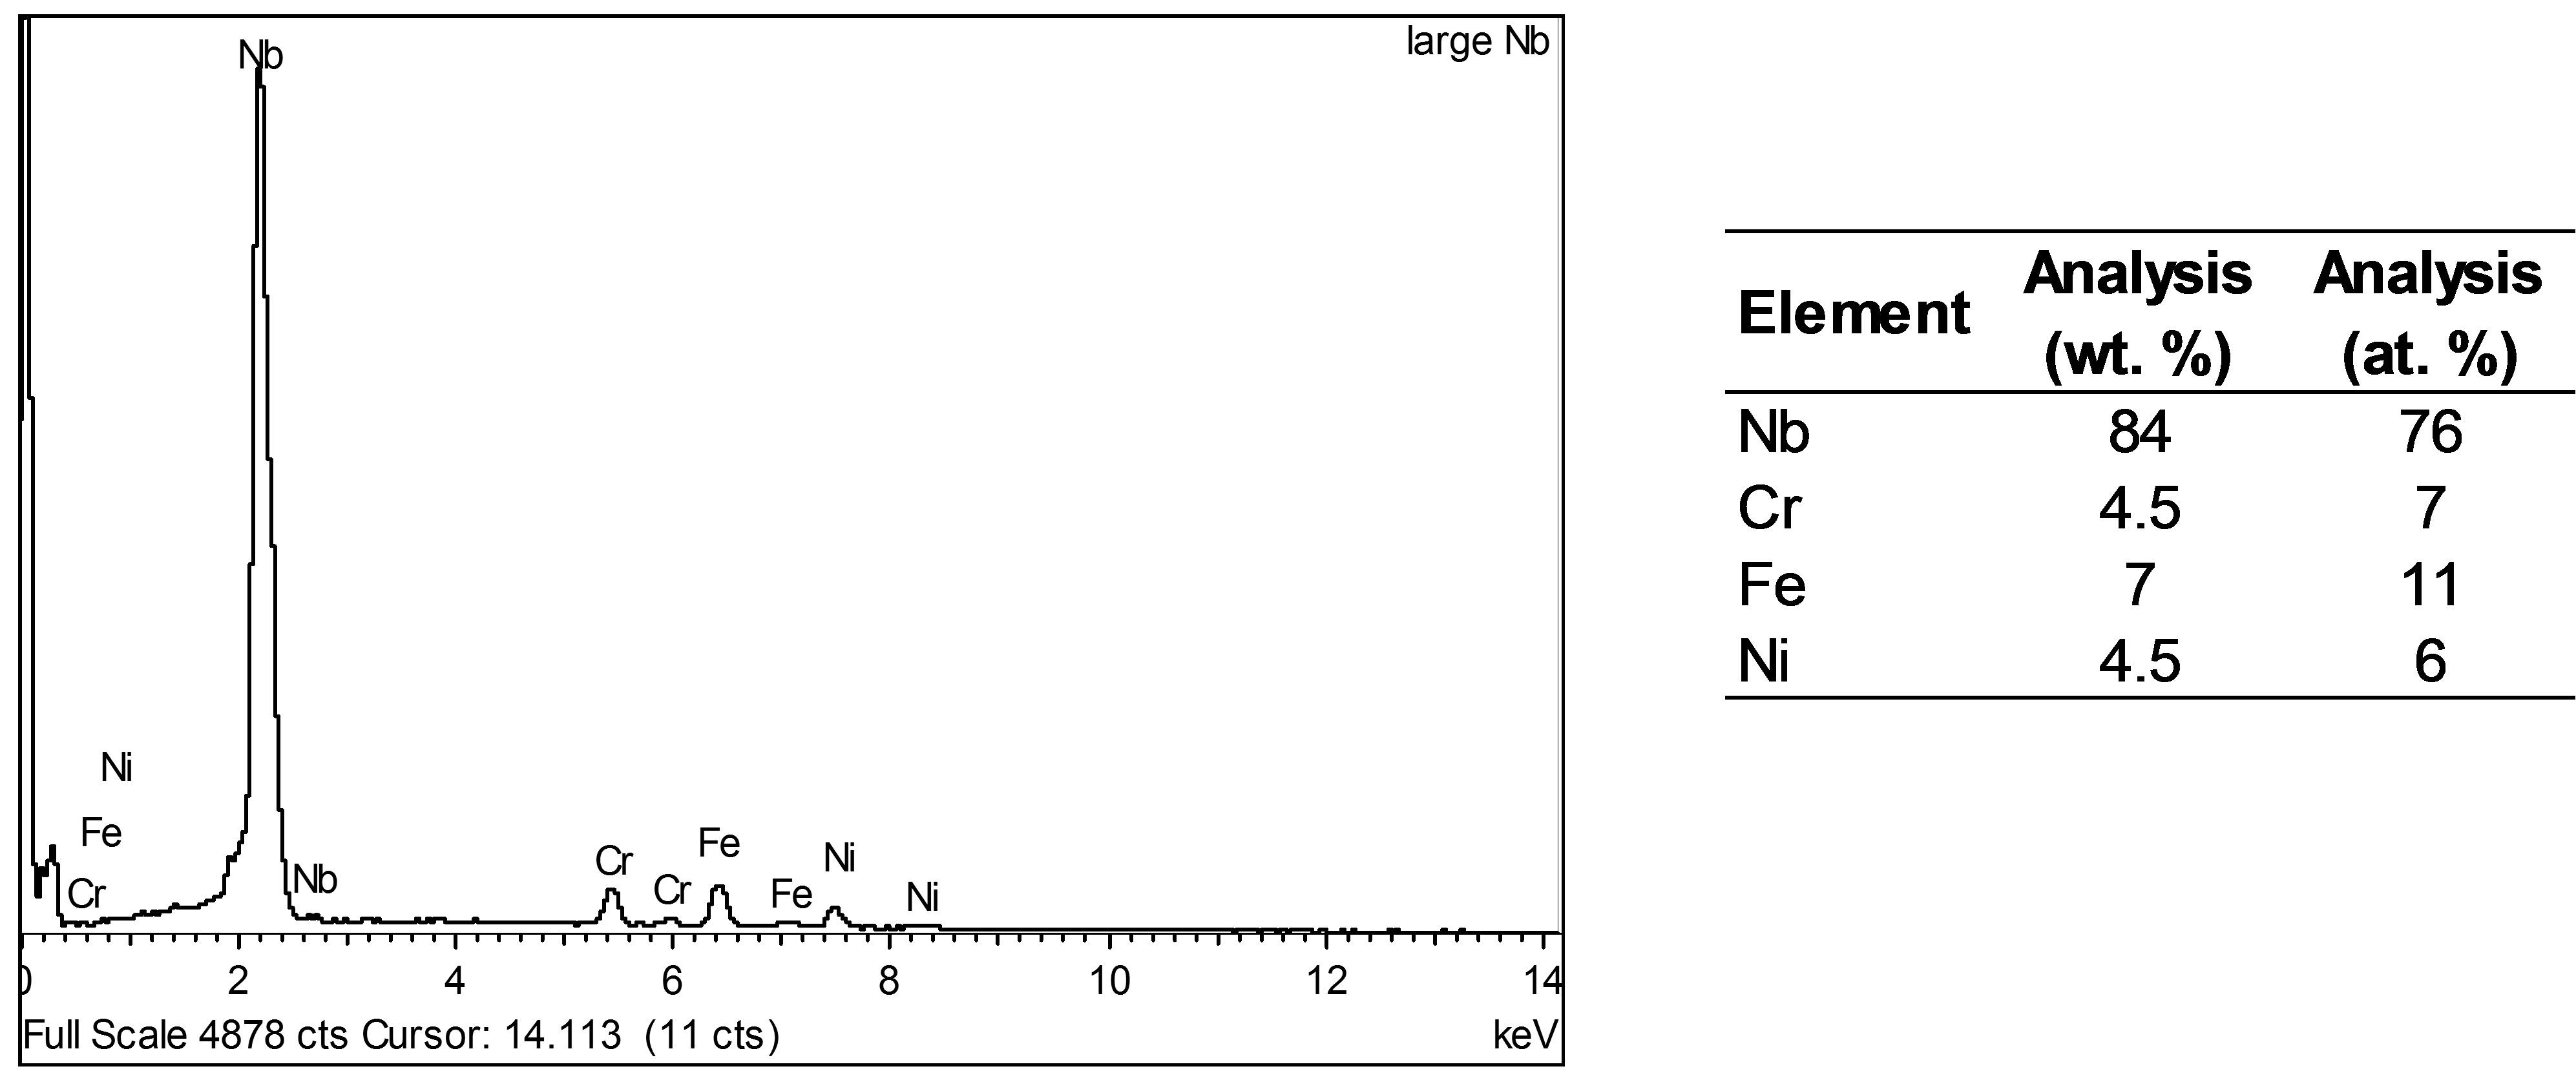
\includegraphics[width=\textwidth]{figures/metallography/c5-ar-eds-table-L1-A.png}} \\
    \subfloat[Spot Analysis ``B'']{\label{subfig:c5-ar-eds-b}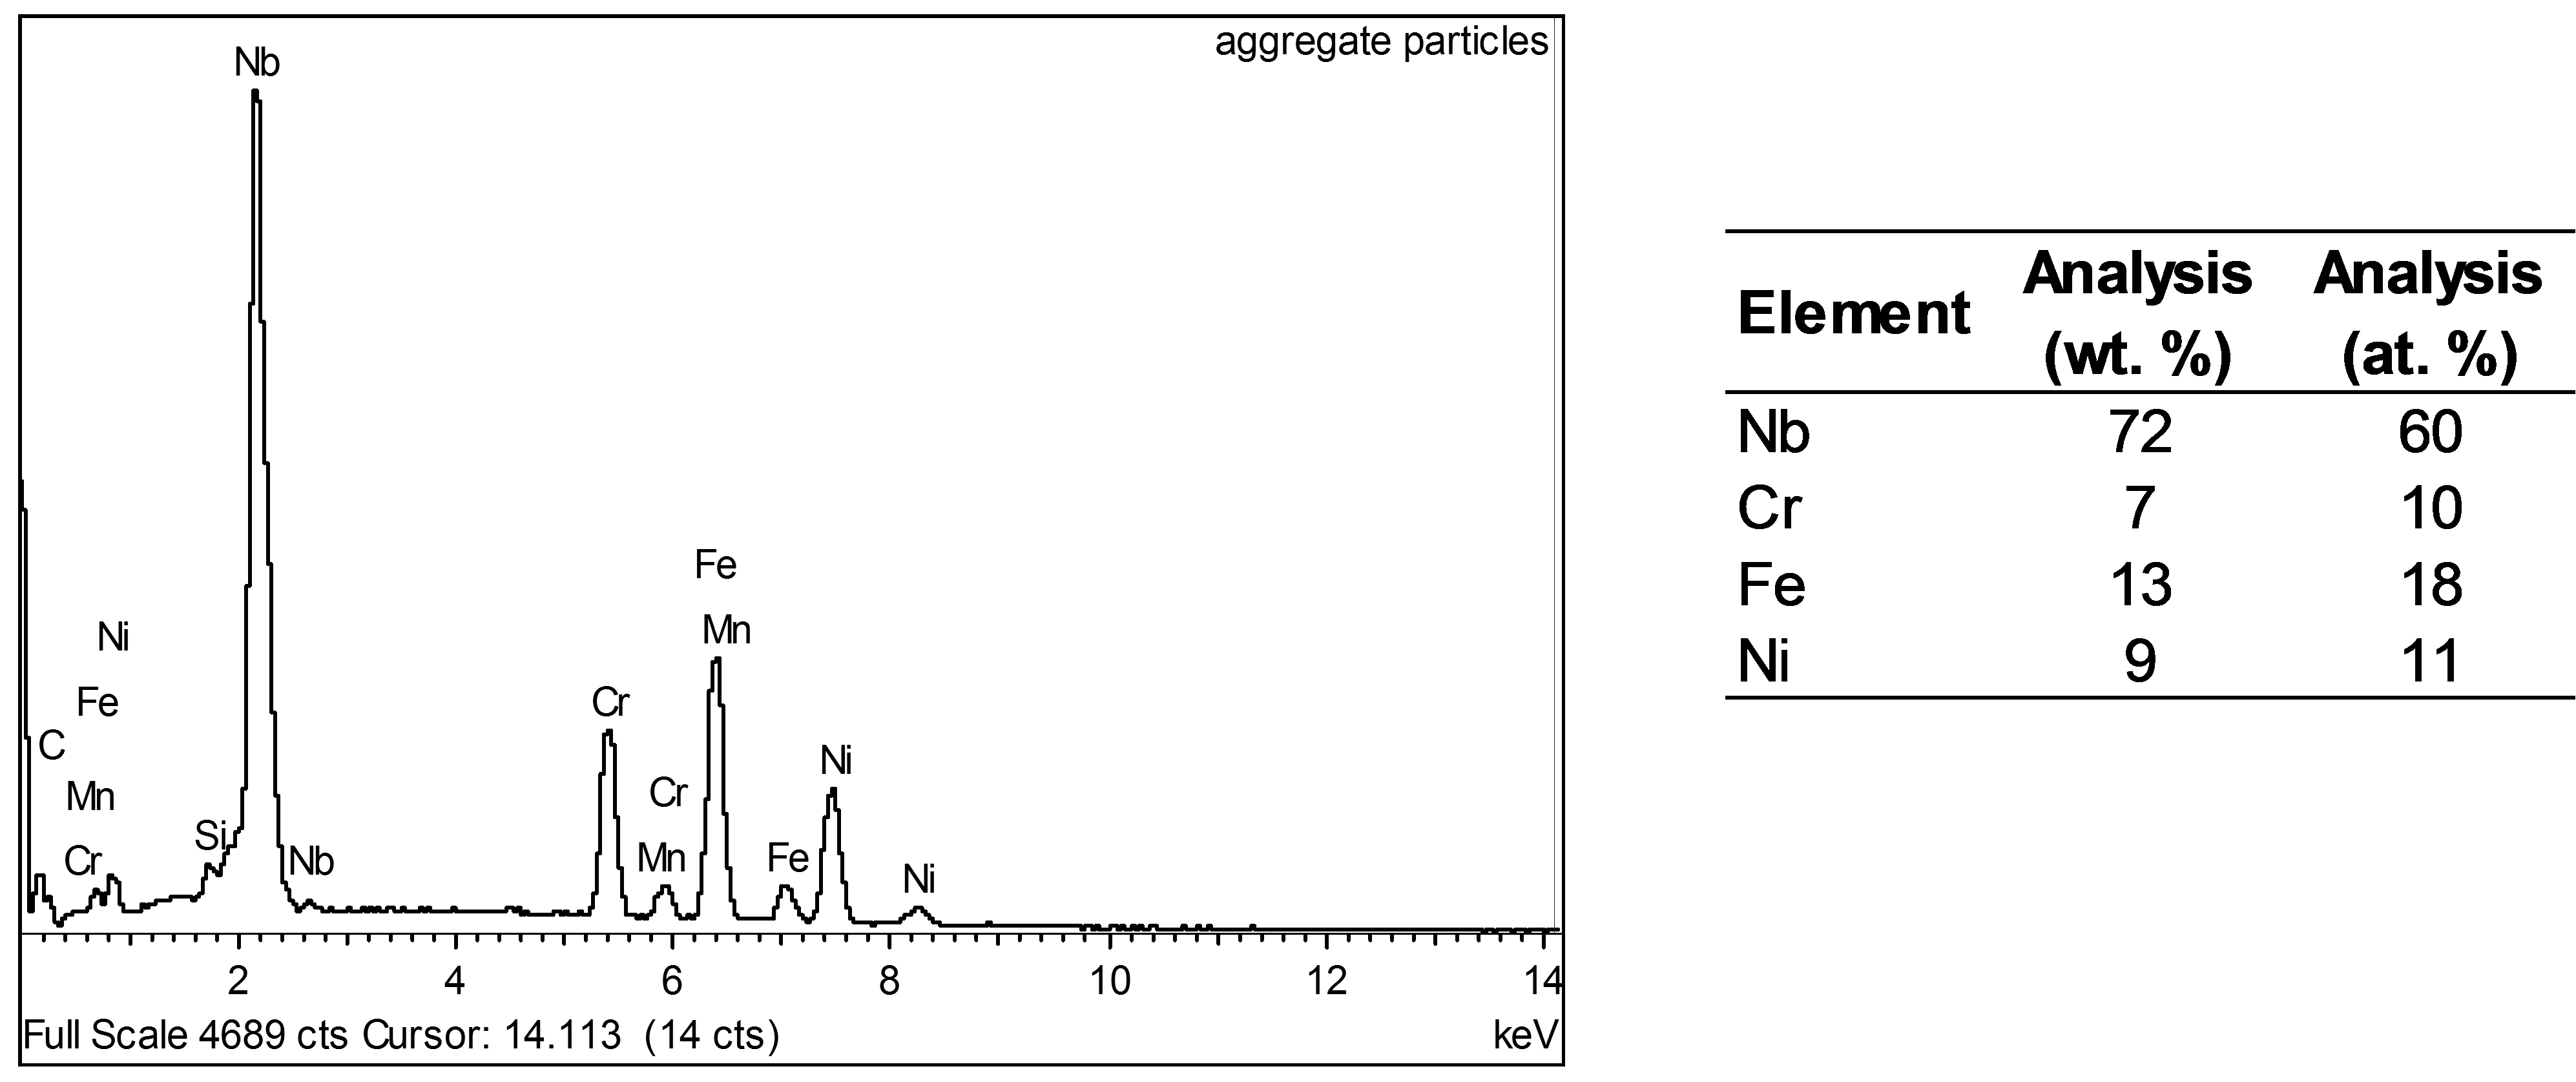
\includegraphics[width=\textwidth]{figures/metallography/c5-ar-eds-table-L1-B.png}}
    \caption[]{\Gls{eds} spot analysis results for locations ``A'' and ``B'' identified in Figure~\ref{subfig:c5-ar-sem-5kx} for as-received Cone~5 material.}
    \label{fig:c5-ar-eds}
\end{figure}


\subsection{Characterization of On-Heating Hot Ductility Tests}
\subsubsection{Cone~1 On-Heating}
Figure~\ref{fig:c1-oh-2375} shows a region adjacent to the fracture surface of the Cone~1 On-Heating 2375\textdegree{}F (C1 OH-2375) hot ductility sample. The C1 OH-2375 sample corresponds to the \gls{zdt} for Cone~1 and significant cracking is evident near the surface with the crack paths following the interdendritic boundaries. Note that in Figure~\ref{fig:c1-oh-2375}, the tensile loading direction for the hot ductility test is in the vertical direction, so the crack paths are oriented perpendicular to the loading direction. It is also apparent that compared to the as-received Cone~1 microstructure (Figure~\ref{fig:c1-asreceived}), dissolution of most of the fine intradendritic precipitates has occurred due to the high temperature of the simulated thermal cycle of the hot ductility test.

The tip of the crack visible in Figure~\ref{subfig:c1-oh-2375-50x} is shown at higher magnification in Figure~\ref{subfig:c1-oh-2375-500X}, which shows evidence of liquation (where liquid was present) along the crack faces, as well as the interdendritic boundary and associated phases ahead of the crack. The liquated regions (where localized melting occurred during the simulated thermal cycle) are denoted by arrows in Figure~\ref{subfig:c1-oh-2375-500X} and are visible as slightly brighter regions which stand faintly in relief. The evidence of prior liquid along the interdendritic boundaries (i.e.~liquated boundaries) correlates with the observed zero ductility behavior observed at this temperature. As the peak temperature of the simulated thermal cycle increases to the point where the first liquid (which cannot support strain) is formed along the boundaries, the ductility will drop to zero. Larger liquated regions are also apparent at other locations near the fracture surface in the C1 OH-2375 sample, as shown in Figure~\ref{fig:c1-oh-2375-fracture-liquation}. However, in general, evidence of liquation is only intermittently present along the fracture profile of the sample shown in Figure~\ref{subfig:c1-oh-2375-50x}. The melted region from Figure~\ref{fig:c1-oh-2375-fracture-liquation} is shown at higher magnification in the \gls{sem} micrograph in Figure~\ref{fig:c1-oh-2375-fracture-liquation-sem} along with spot \gls{eds} results for a location in the liquated region. It is apparent that the liquated region, surrounding the interdendritic phases along a boundary, is not enriched in Ni, Nb, or Si which is in agreement with the results for the as-received Cone 1 base metal which did not find evidence of Ni-Nb-Si-rich phases surrounding the eutectic NbC.

%Figures for C1 OH-2375
\begin{figure}
    \centering
    \subfloat[50X]{\label{subfig:c1-oh-2375-50x}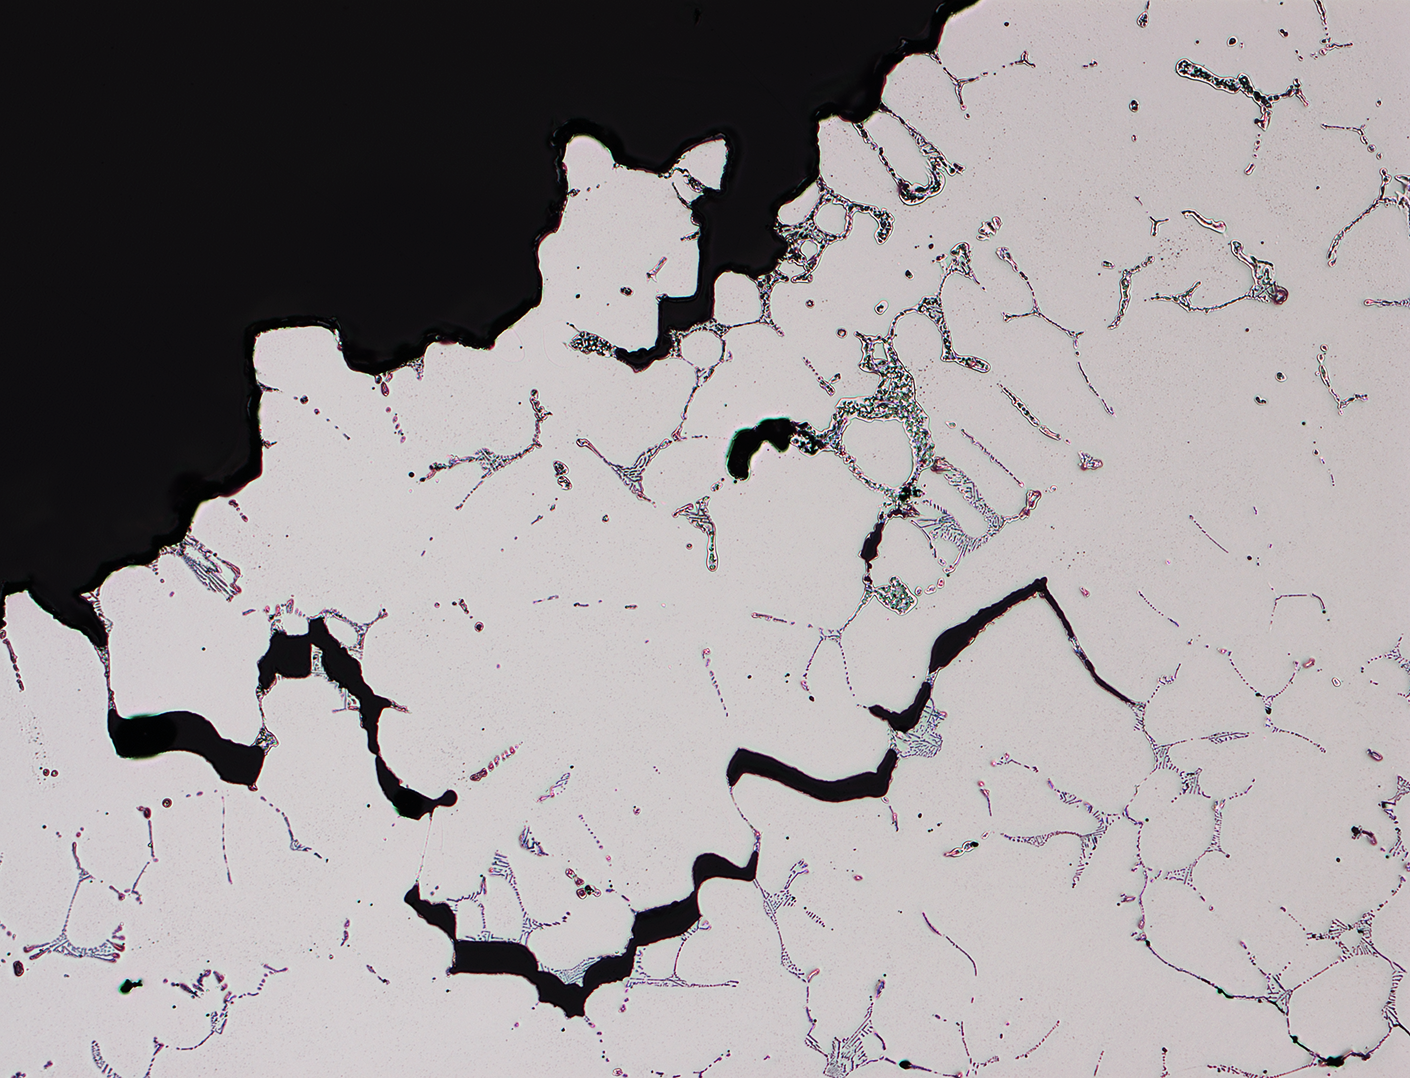
\includegraphics[width=4.7in]{figures/metallography/c1-oh-2375-50x.png}} \\
    \subfloat[500X]{\label{subfig:c1-oh-2375-500X}\includegraphics[width=4.7in]{figures/metallography/c1-oh-2375-crack-500x.png}}
    \caption{Optical micrographs showing the region adjacent to the fracture surface in the Cone~1 On-Heating 2375\textdegree{}F (C1 OH-2375) hot ductility sample. Evidence of liquation (where melting occurred during the simulated thermal cycle) is denoted by arrows. Etch: electrolytic 10\% oxalic acid.}
    \label{fig:c1-oh-2375}
\end{figure}

\begin{figure}
    \centering
    \subfloat[100X]{\label{subfig:c1-oh-2375-liquation-100x}\includegraphics[width=4.7in]{figures/metallography/c1-oh-2375-fracture-liquation-100x.png}} \\
    \subfloat[500X]{\label{subfig:c1-oh-2375-liquation-500X}\includegraphics[width=4.7in]{figures/metallography/c1-oh-2375-fracture-liquation-500x.png}}
    \caption{Optical micrographs showing liquation around interdendritic phases adjacent to the fracture surface in the Cone~1 On-Heating 2375\textdegree{}F (C1 OH-2375) hot ductility sample. Etch: electrolytic 10\% oxalic acid.}
    \label{fig:c1-oh-2375-fracture-liquation}
\end{figure}

\begin{figure}
    \centering
    \subfloat[SEM micrograph of liquated region]{\label{subfig:c1-oh-2375-sem-2.5kx}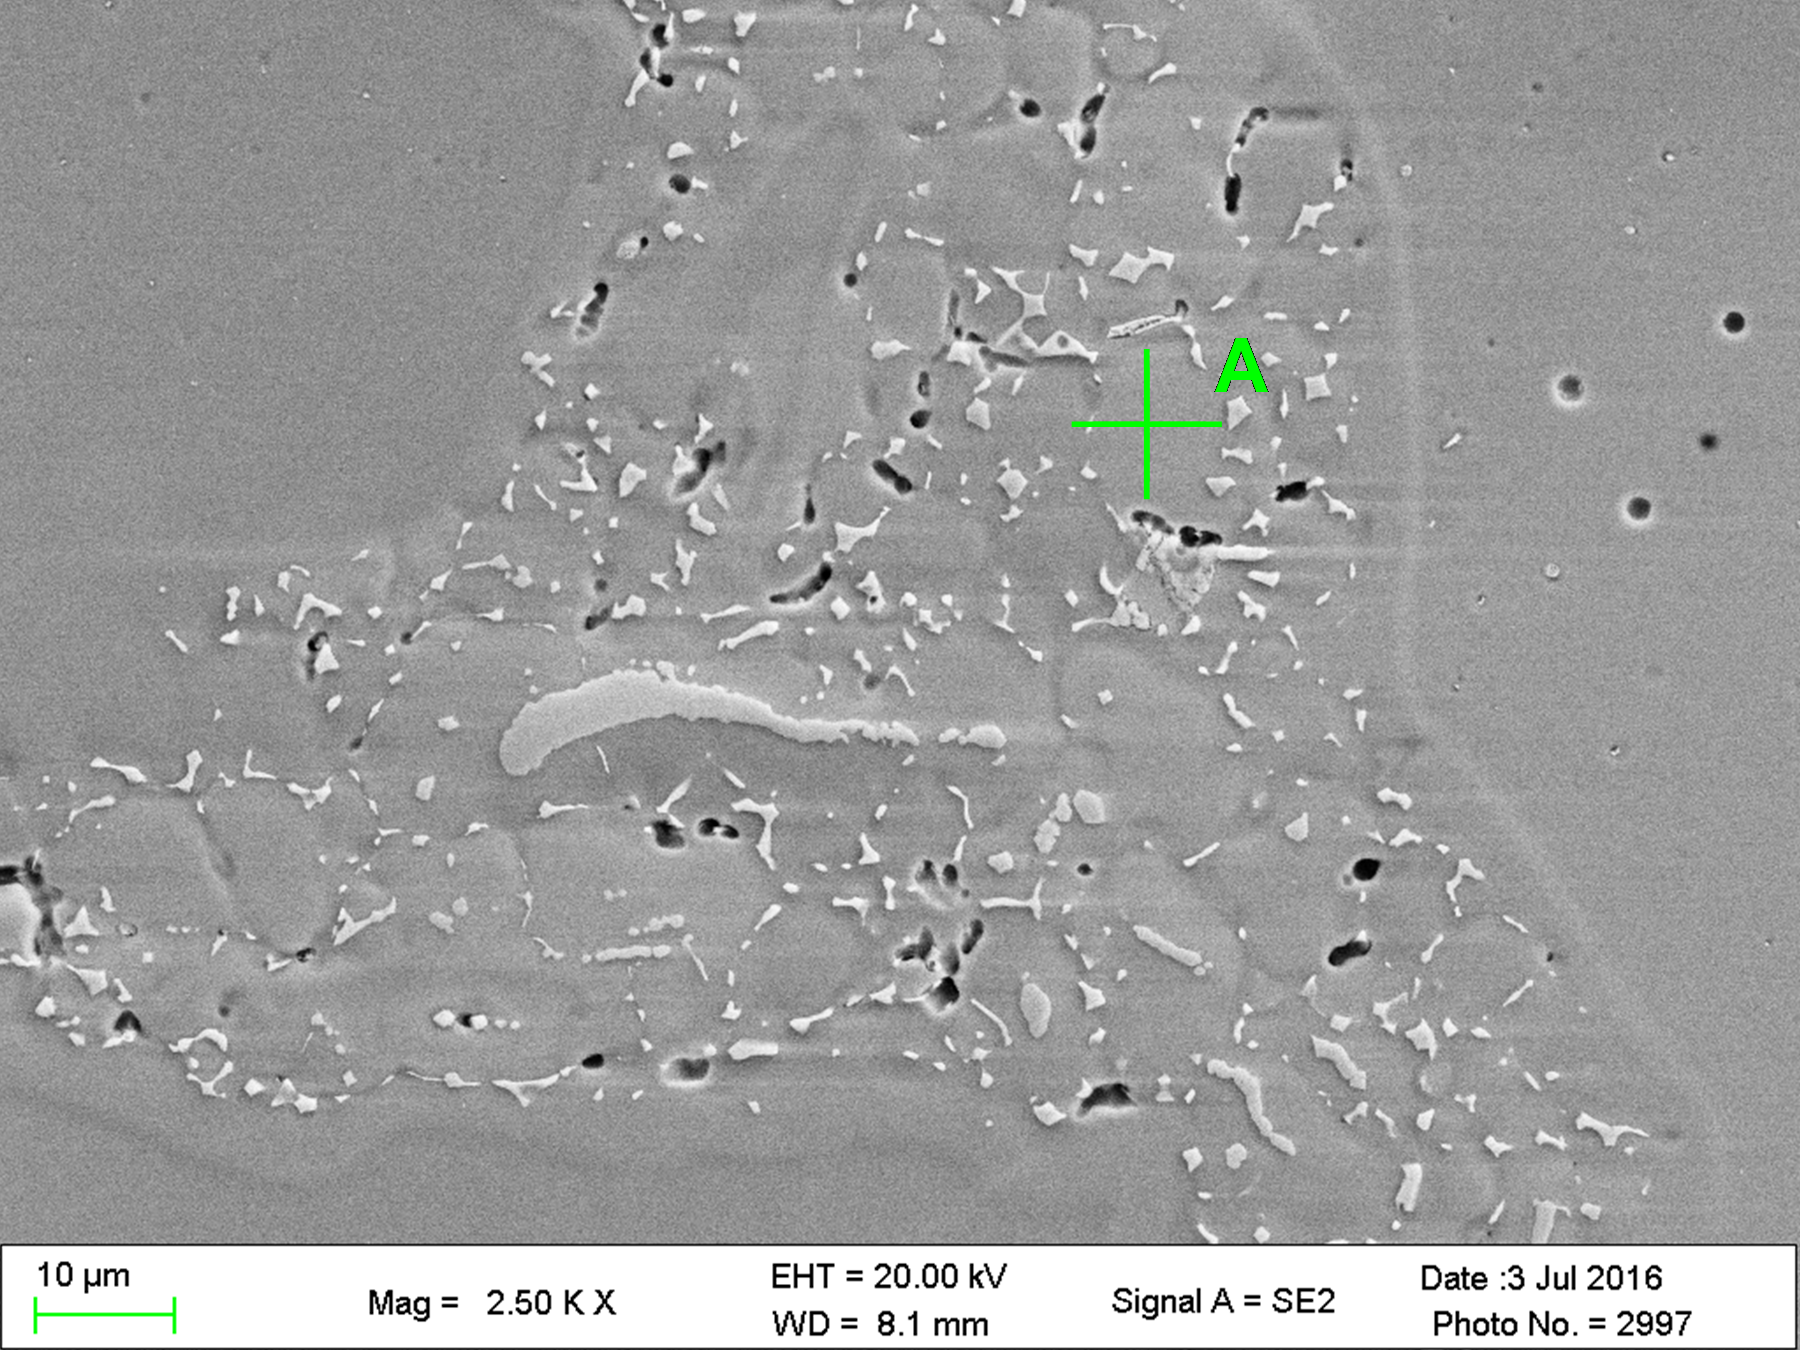
\includegraphics[width=4.7in]{figures/metallography/c1-oh-2375-liquation-sem.png}} \\
    \subfloat[Spot \gls{eds} results for point ``A'']{\label{subfig:c1-oh-2375-liquation-eds}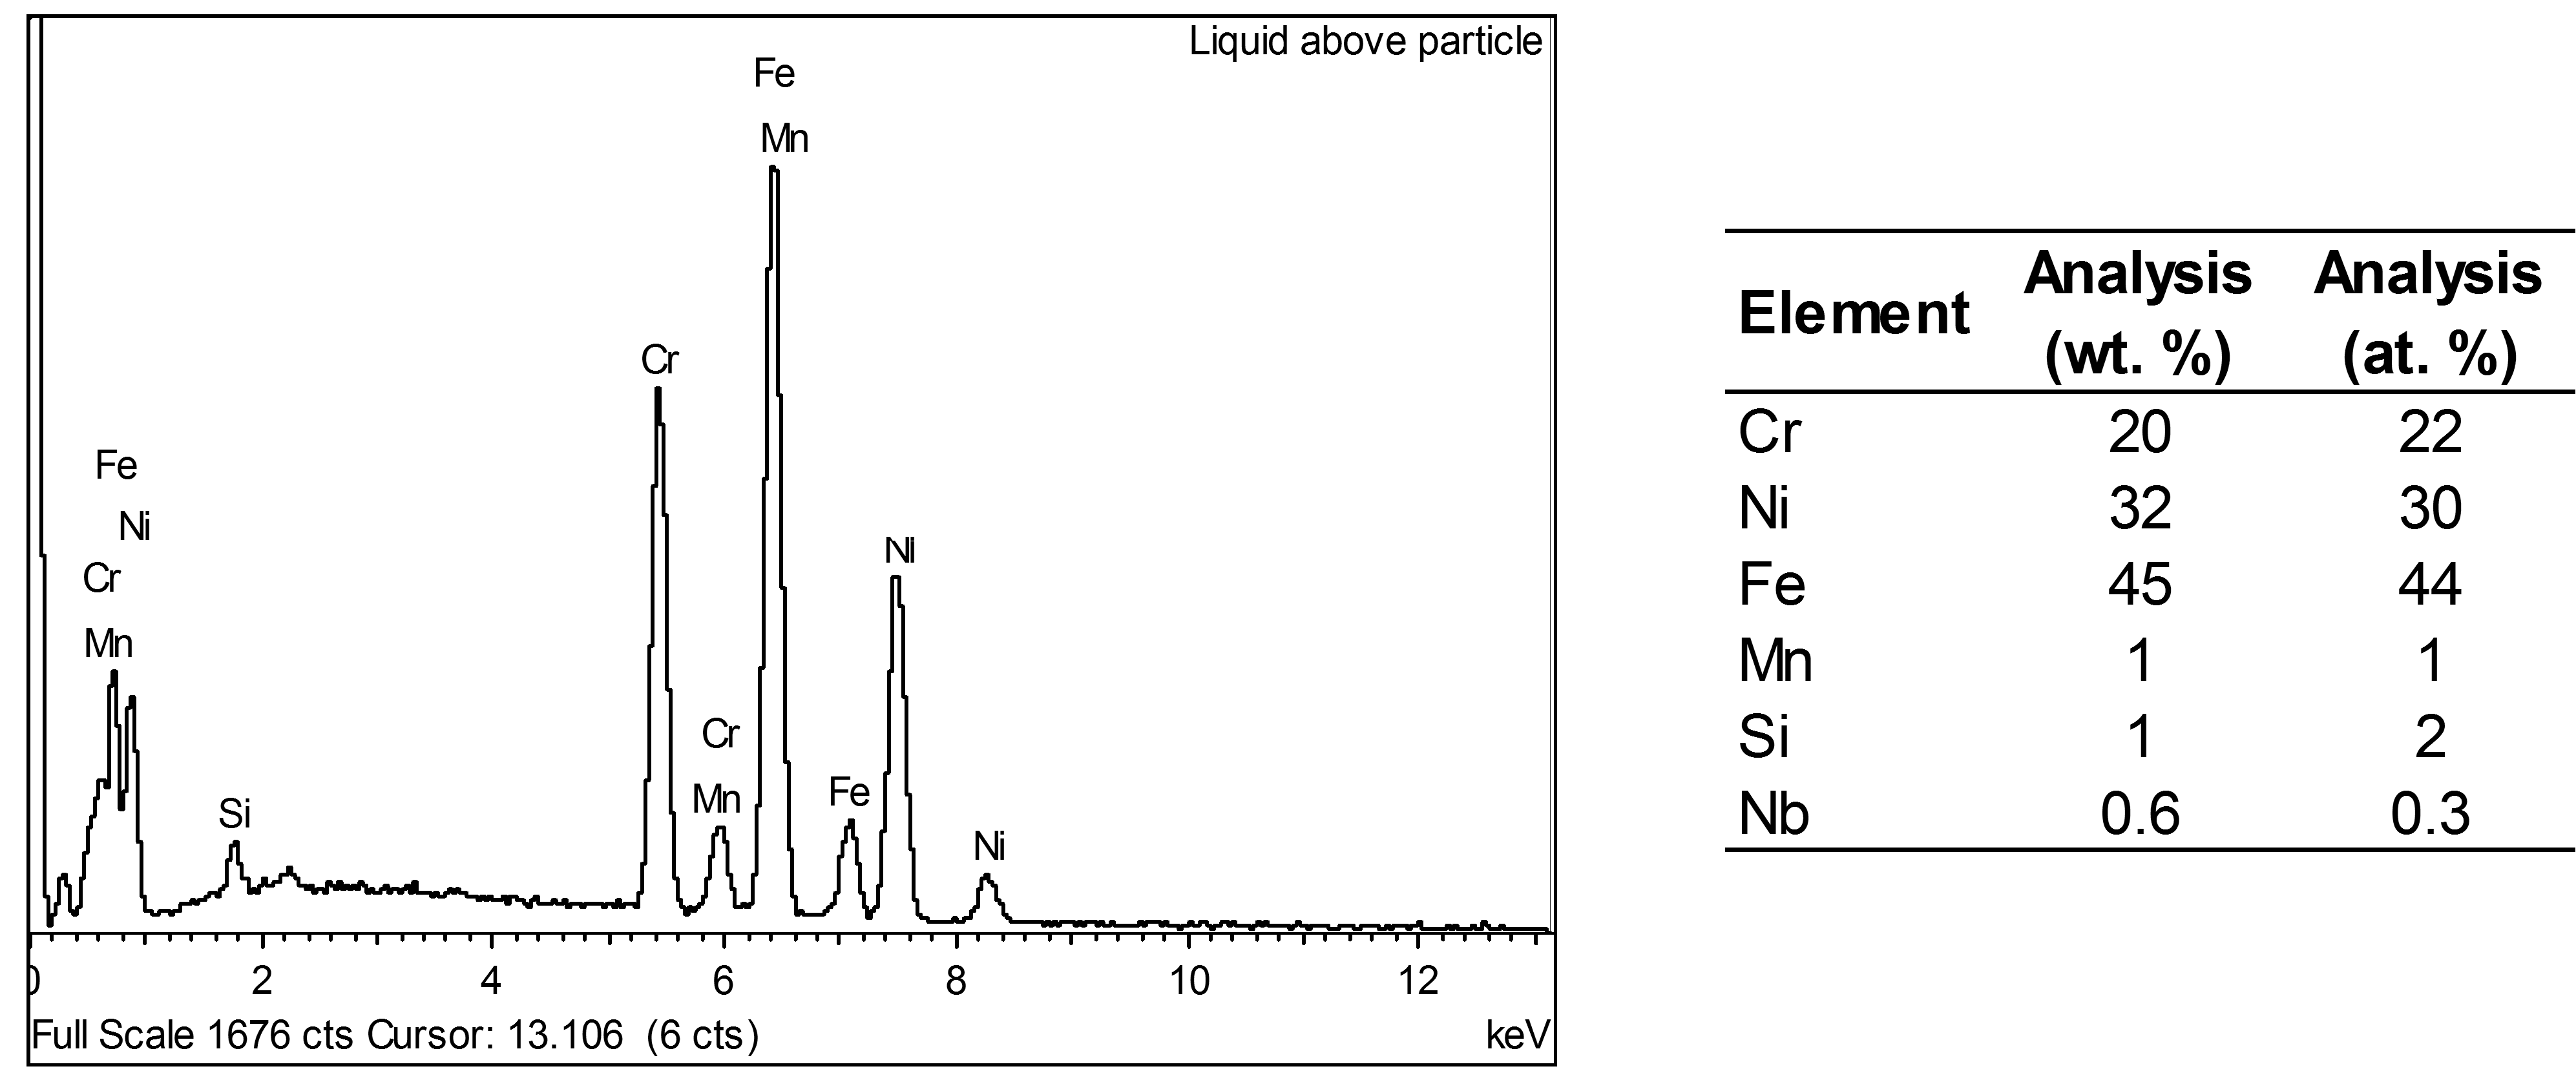
\includegraphics[width=\textwidth]{figures/metallography/c1-oh-2375-liquation-eds-table.png}}
    \caption{\Gls{sem} micrograph showing liquation around interdendritic phases adjacent to the fracture surface in the Cone~1 On-Heating 2375\textdegree{}F (C1 OH-2375) hot ductility sample with spot \gls{eds} results for indicated point ``A'' within the melted region. Etch: electrolytic 10\% oxalic acid.}
    \label{fig:c1-oh-2375-fracture-liquation-sem}
\end{figure}
\clearpage
%Need some EDS of phases in front of crack, e.g. NbC

\subsubsection{Cone~5 On-Heating}
Figure~\ref{fig:c5-oh-2375-olm-fracture} shows a region at the fracture surface of the Cone~5 On-Heating 2375\textdegree{}F (C5 OH-2375) hot ductility sample which corresponds to the \gls{zdt} of Cone~5. As with Cone~1, cracking is evident along the interdendritic boundaries and a majority of the intradendritic precipitates have dissolved due to the high temperature exposure. The crack tip is shown in Figure~\ref{fig:c5-oh-2375-crack-100x} and two separate regions at the tip of the crack shown in Figure~\ref{fig:c5-oh-2375-crack-100x} are shown at higher magnification in Figure~\ref{fig:c5-oh-2375-crack-tip-500x}. It is apparent that liquated regions (where liquid was formed during the simulated thermal cycle) exist along a portion of the crack faces and around some of the interdendritic phases ahead of the crack (see arrows in Figure~\ref{subfig:c5-oh-2375-wide-crack-500x}). However, significant evidence of prior liquid is not apparent at the extreme tip portion where the crack is quite narrow (Figure~\ref{subfig:c5-oh-2375-narrow-crack-500x}), indicating that minimal to no liquid was formed at this location during the simulated thermal cycle. Similarly to Cone~1, liquated regions are visible at other locations adjacent to the fracture surface away from apparent cracks, as shown in Figure~\ref{fig:c5-oh-2375-liquation-fracture-surface}. Again, the liquated regions are not present continuously along the fracture profile, indicating a lesser extent of prior liquid formation (as compared to the on-cooling tests which will be discussed later). Overall, both Cone~1 and Cone~5 show a similar hot ductility response in the on-heating tests.

%[C5 OH-2375 SEM to be added]

%Figures for C5 OH-2375
\begin{figure}
    \centering
    \includegraphics[width=\textwidth]{figures/metallography/c5-oh-2375-olm-fracture-50x.png}
    \caption{Optical micrograph showing cracking and liquation in a region adjacent to the fracture surface in the Cone~5 On-Heating 2375\textdegree{}F (C5 OH-2375) hot ductility sample. The crack tip region is shown in Figure~\ref{fig:c5-oh-2375-crack-100x}. Etch: electrolytic 10\% oxalic acid.}
    \label{fig:c5-oh-2375-olm-fracture}
\end{figure}

\begin{figure}
    \centering
    \includegraphics[width=\textwidth]{figures/metallography/c5-oh-2375-crack-100x.png}
    \caption{Optical micrograph of the tip of the crack visible in Figure~\ref{fig:c5-oh-2375-olm-fracture}. The crack tip region is shown at higher magnification in Figure~\ref{fig:c5-oh-2375-crack-tip-500x}. Etch: electrolytic 10\% oxalic acid.}
    \label{fig:c5-oh-2375-crack-100x}
\end{figure}

\begin{figure}
    \centering
    \subfloat[Wider region near crack tip]{\label{subfig:c5-oh-2375-wide-crack-500x}\includegraphics[width=4.7in]{figures/metallography/c5-oh-2375-wide-crack-500x.png}} \\
    \subfloat[Narrower region at crack tip]{\label{subfig:c5-oh-2375-narrow-crack-500x}\includegraphics[width=4.7in]{figures/metallography/c5-oh-2375-narrow-crack-500x.png}}
    \caption{Optical micrographs showing wide and narrow regions at the tip of the crack visible in Figure~\ref{fig:c5-oh-2375-crack-100x}. Liquation around the interdendritic phases and on the crack faces is evident in (a), as indicated by arrows, but not in (b). Etch: electrolytic 10\% oxalic acid.}
    \label{fig:c5-oh-2375-crack-tip-500x}
\end{figure}

\begin{figure}
    \centering
    \subfloat[100X]{\label{subfig:c5-oh-2375-liquation-100x}\includegraphics[width=4.7in]{figures/metallography/c5-oh-2375-liquation-100x.png}} \\
    \subfloat[500X]{\label{subfig:c5-oh-2375-liquation-500x}\includegraphics[width=4.7in]{figures/metallography/c5-oh-2375-liquation-500x.png}}
    \caption{Optical micrographs showing evidence of liquation around interdendritic phases near the fracture surface in the Cone~5 On-Heating 2375\textdegree{}F (C5 OH-2375) hot ductility sample. Etch: electrolytic 10\% oxalic acid.}
    \label{fig:c5-oh-2375-liquation-fracture-surface}
\end{figure}
\clearpage


\subsection{Characterization of On-Cooling Hot Ductility Tests}
\subsubsection{Cone~1 On-Cooling}
The near-surface region of the Cone~1 On-Cooling 2300F (C1 OC-2300) hot ductility sample is shown in Figure~\ref{fig:c1-oc-2300-fracture-panorama}. As with the C1 OH-2375 test (Figure~\ref{fig:c1-oh-2375}), cracking is readily apparent with the crack paths following the interdendritic boundaries, and a significant fraction of the intradendritic precipitates have dissolved. However, compared with the C1 OH-2375 sample, the C1 OC-2300 sample exhibits a much larger extent of prior liquid formation near the fracture surface, which is apparent in Figure~\ref{fig:c1-oc-2300-fracture-panorama} and also at higher magnification in Figure~\ref{fig:c1-oc-2300-liquation-surface} (see arrows). In these micrographs the prior liquid films are nearly continuous across the fracture surface. The greater extent of liquation is due to the longer duration of elevated temperature exposure for this sample, even though C1 OH-2375 and C1 OC-2300 experienced the same peak temperature (recall that the peak temperature for the on-cooling tests was chosen as the on-heating \gls{zdt}, equal to 2375\textdegree{}F). In the on-cooling tests, the sample spends a short though definite amount of time near the peak of the welding thermal cycle before being fractured on-cooling, with the precise time (1.4 s above 2360\textdegree{}F, for the thermal cycle utilized herein) dependent on the welding parameters and corresponding thermal cycle characteristics. In comparison, the on-heating \gls{zdt} sample (C1 OH-2375) was fractured immediately upon reaching the peak temperature with correspondingly less time for liquid formation.

Figure~\ref{fig:c1-oc-2300-crack-region-200x} presents a higher magnification view of the region near the tip of the crack shown in Figure~\ref{fig:c1-oc-2300-fracture-panorama}. Extensive liquated regions are apparent around the interdendritic phases and along the crack faces. The crack tip region is shown in the SEM micrographs in Figure~\ref{fig:c1-oc-2300-crack-sem}, with the corresponding EDS analysis results (from the box in Figure~\ref{subfig:c1-oc-2300-crack-5kx}) given in Figure~\ref{fig:c1-oc-2300-crack-tip-particles-eds}. There are numerous small particles located on the crack faces and on the interdendritic boundary ahead of the crack tip, which are enriched in Nb (Figure~\ref{fig:c1-oc-2300-crack-tip-particles-eds}); the Fe, Cr, and Ni peaks most likely originate from the surrounding matrix. Notably, Si enrichment above the nominal alloy composition is not observed which indicates the Ni-Nb-Si silicide phase is not present in the interdendritic region depicted here. 

The liquated region surrounding some of the interdendritic phases in Figure~\ref{fig:c1-oc-2300-fracture-panorama} is evaluated further in the SEM micrographs in Figure~\ref{fig:c1-oc-2300-sem-liquid} with corresponding EDS spot analysis results in Figure~\ref{fig:c1-oc-2300-liquid-eds}. The quantitative EDS results indicate that the white particle is NbC while the surrounding prior liquid (around the interdendritic phases) is essentially similar to the nominal alloy composition and is not enriched in Ni, Nb, or Si. This fact suggests that the formation of prior liquid in this region (along the interdendritic boundaries) is not due to melting of Ni-Nb-Si phases during the simulated on-cooling thermal cycle.

%C1 On-cooling figures
\begin{landscape}
\begin{figure}
    \centering
    \includegraphics[width=8in]{figures/metallography/c1-oc-2300-fracture-panorama.png}
    \caption{Optical micrograph of a region of the fracture surface in the Cone~1 On-Cooling 2300\textdegree{}F (C1 OC-2300) hot ductility sample. Note the extensive formation of liquated regions near the surface (e.g. as denoted by arrows). Original magnification, 50X. Etch: electrolytic 10\% oxalic acid.}
    \label{fig:c1-oc-2300-fracture-panorama}
\end{figure}
\end{landscape}

\begin{figure}
    \centering
    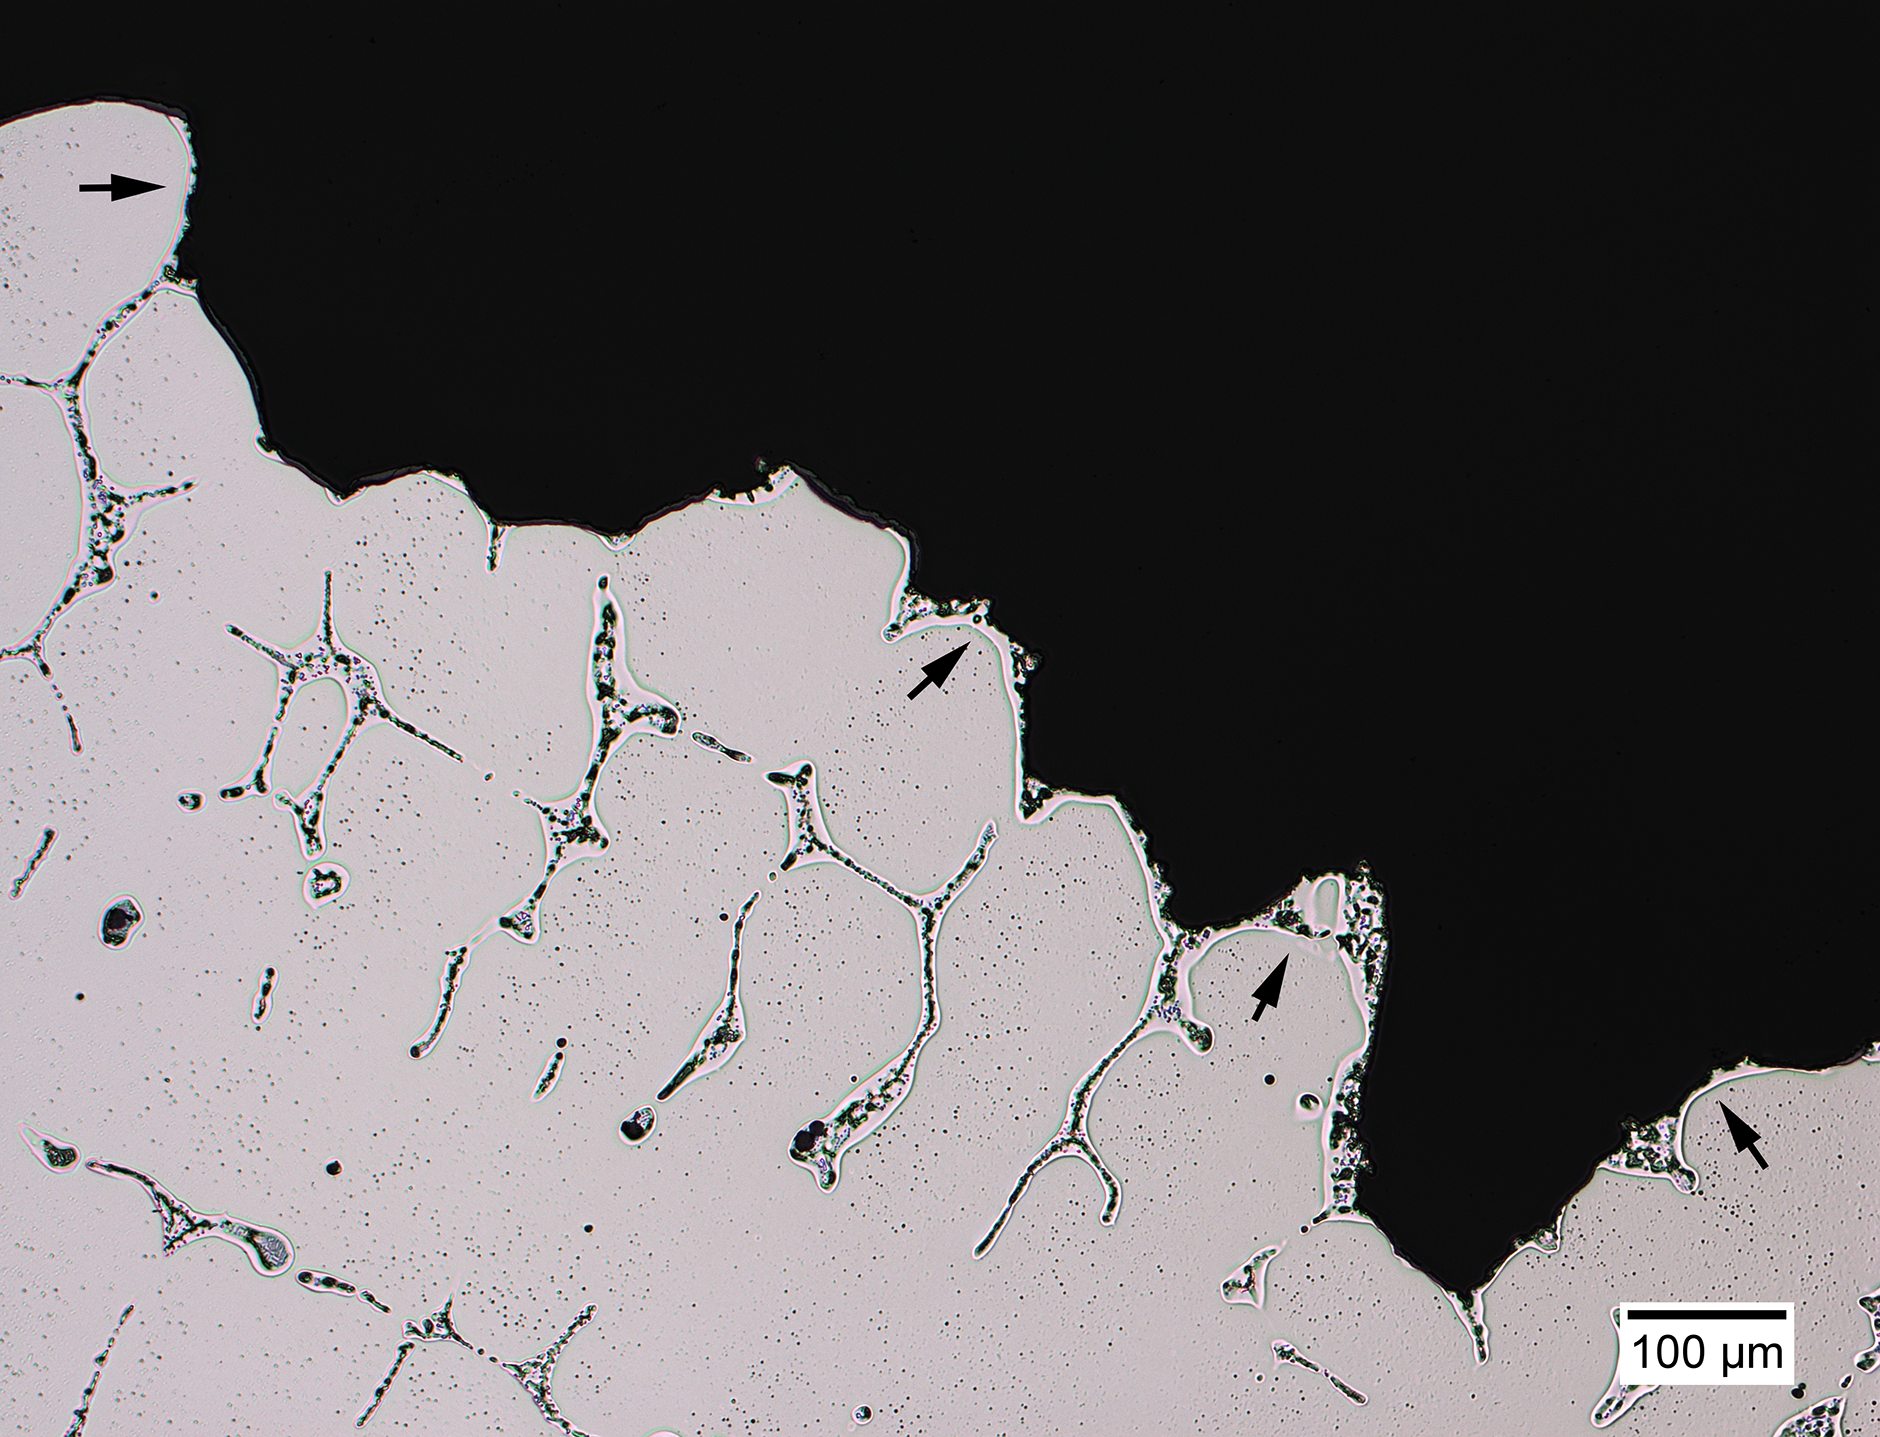
\includegraphics[width=4.7in]{figures/metallography/c1-oc-2300-liquation-surface-100x.png}
    \caption{Optical micrograph showing a nearly continuous film of prior liquid (arrows) along the fracture surface of the Cone~1 On-Cooling 2300\textdegree{}F (C1 OC-2300) hot ductility sample, 100X. Etch: electrolytic 10\% oxalic acid.}
    \label{fig:c1-oc-2300-liquation-surface}
\end{figure}

\begin{figure}
    \centering
    \includegraphics[width=4.7in]{figures/metallography/c1-oc-2300-crack-region-200x.png}
    \caption[]{Optical micrograph showing extensive liquation (arrows) along the crack faces and surrounding interdendritic phases, near the tip of the crack visible in Figure~\ref{fig:c1-oc-2300-fracture-panorama} for the Cone~1 On-Cooling 2300\textdegree{}F (C1 OC-2300) hot ductility sample, 200X. Etch: electrolytic 10\% oxalic acid.}
    \label{fig:c1-oc-2300-crack-region-200x}
\end{figure}

\begin{figure}
    \centering
    \subfloat[1000X]{\label{subfig:c1-oc-2300-crack-1kx}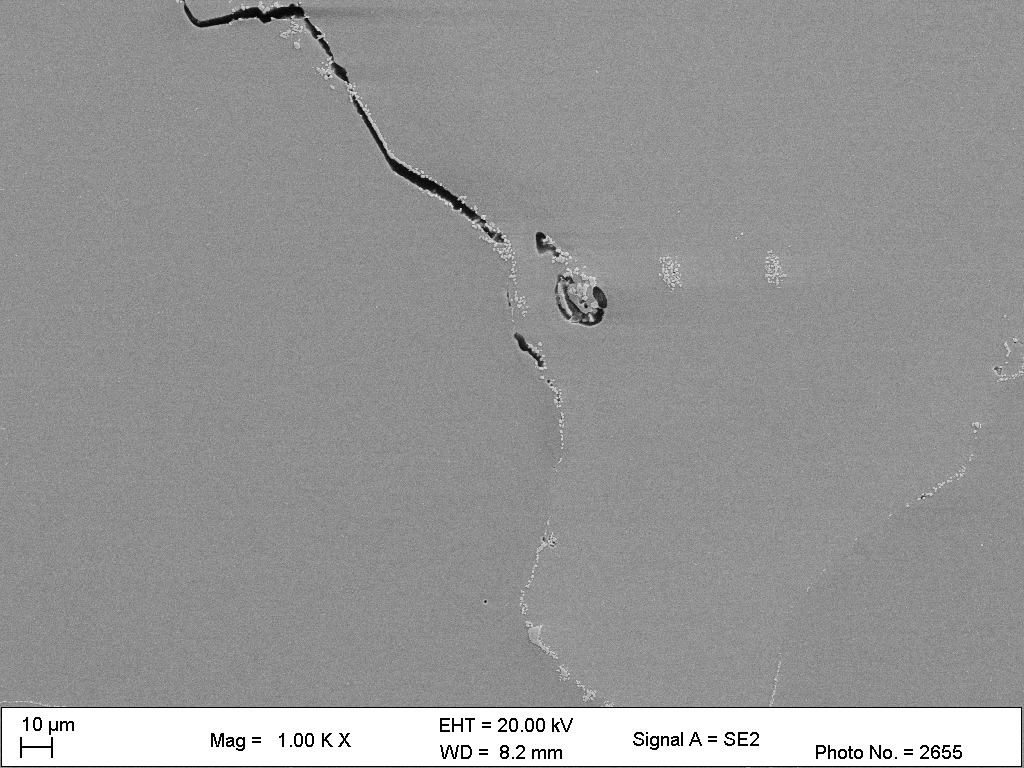
\includegraphics[width=4.7in]{figures/metallography/c1-oc-2300-crack-1kx-L3-17.png}} \\
    \subfloat[5000X]{\label{subfig:c1-oc-2300-crack-5kx}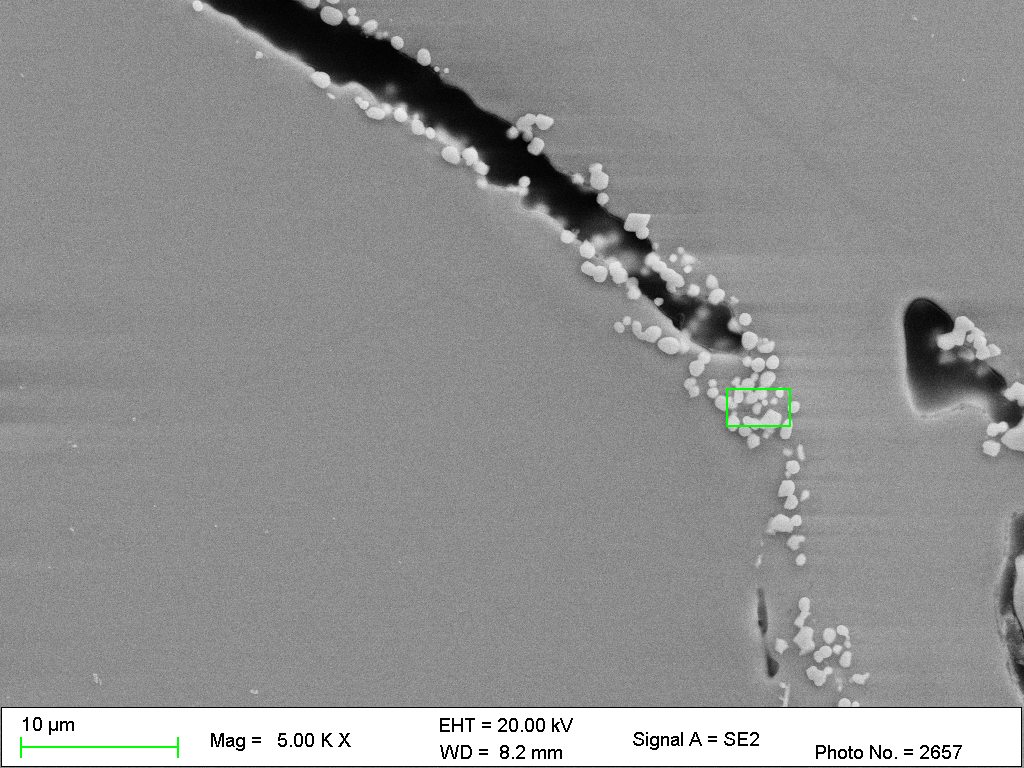
\includegraphics[width=4.7in]{figures/metallography/c1-oc-2300-crack-5kx-L3-19.png}}
    \caption{\Gls{sem} micrographs showing the region at the tip of the crack visible in Figure~\ref{fig:c1-oc-2300-fracture-panorama} for the Cone~5 On-Heating 2375\textdegree{}F (C5 OH-2375) hot ductility sample. The \gls{eds} results for the boxed area in (b) are given in Figure~\ref{fig:c1-oc-2300-crack-tip-particles-eds}. Etch: electrolytic 10\% oxalic acid.}
    \label{fig:c1-oc-2300-crack-sem}
\end{figure}

\begin{figure}
    \centering
    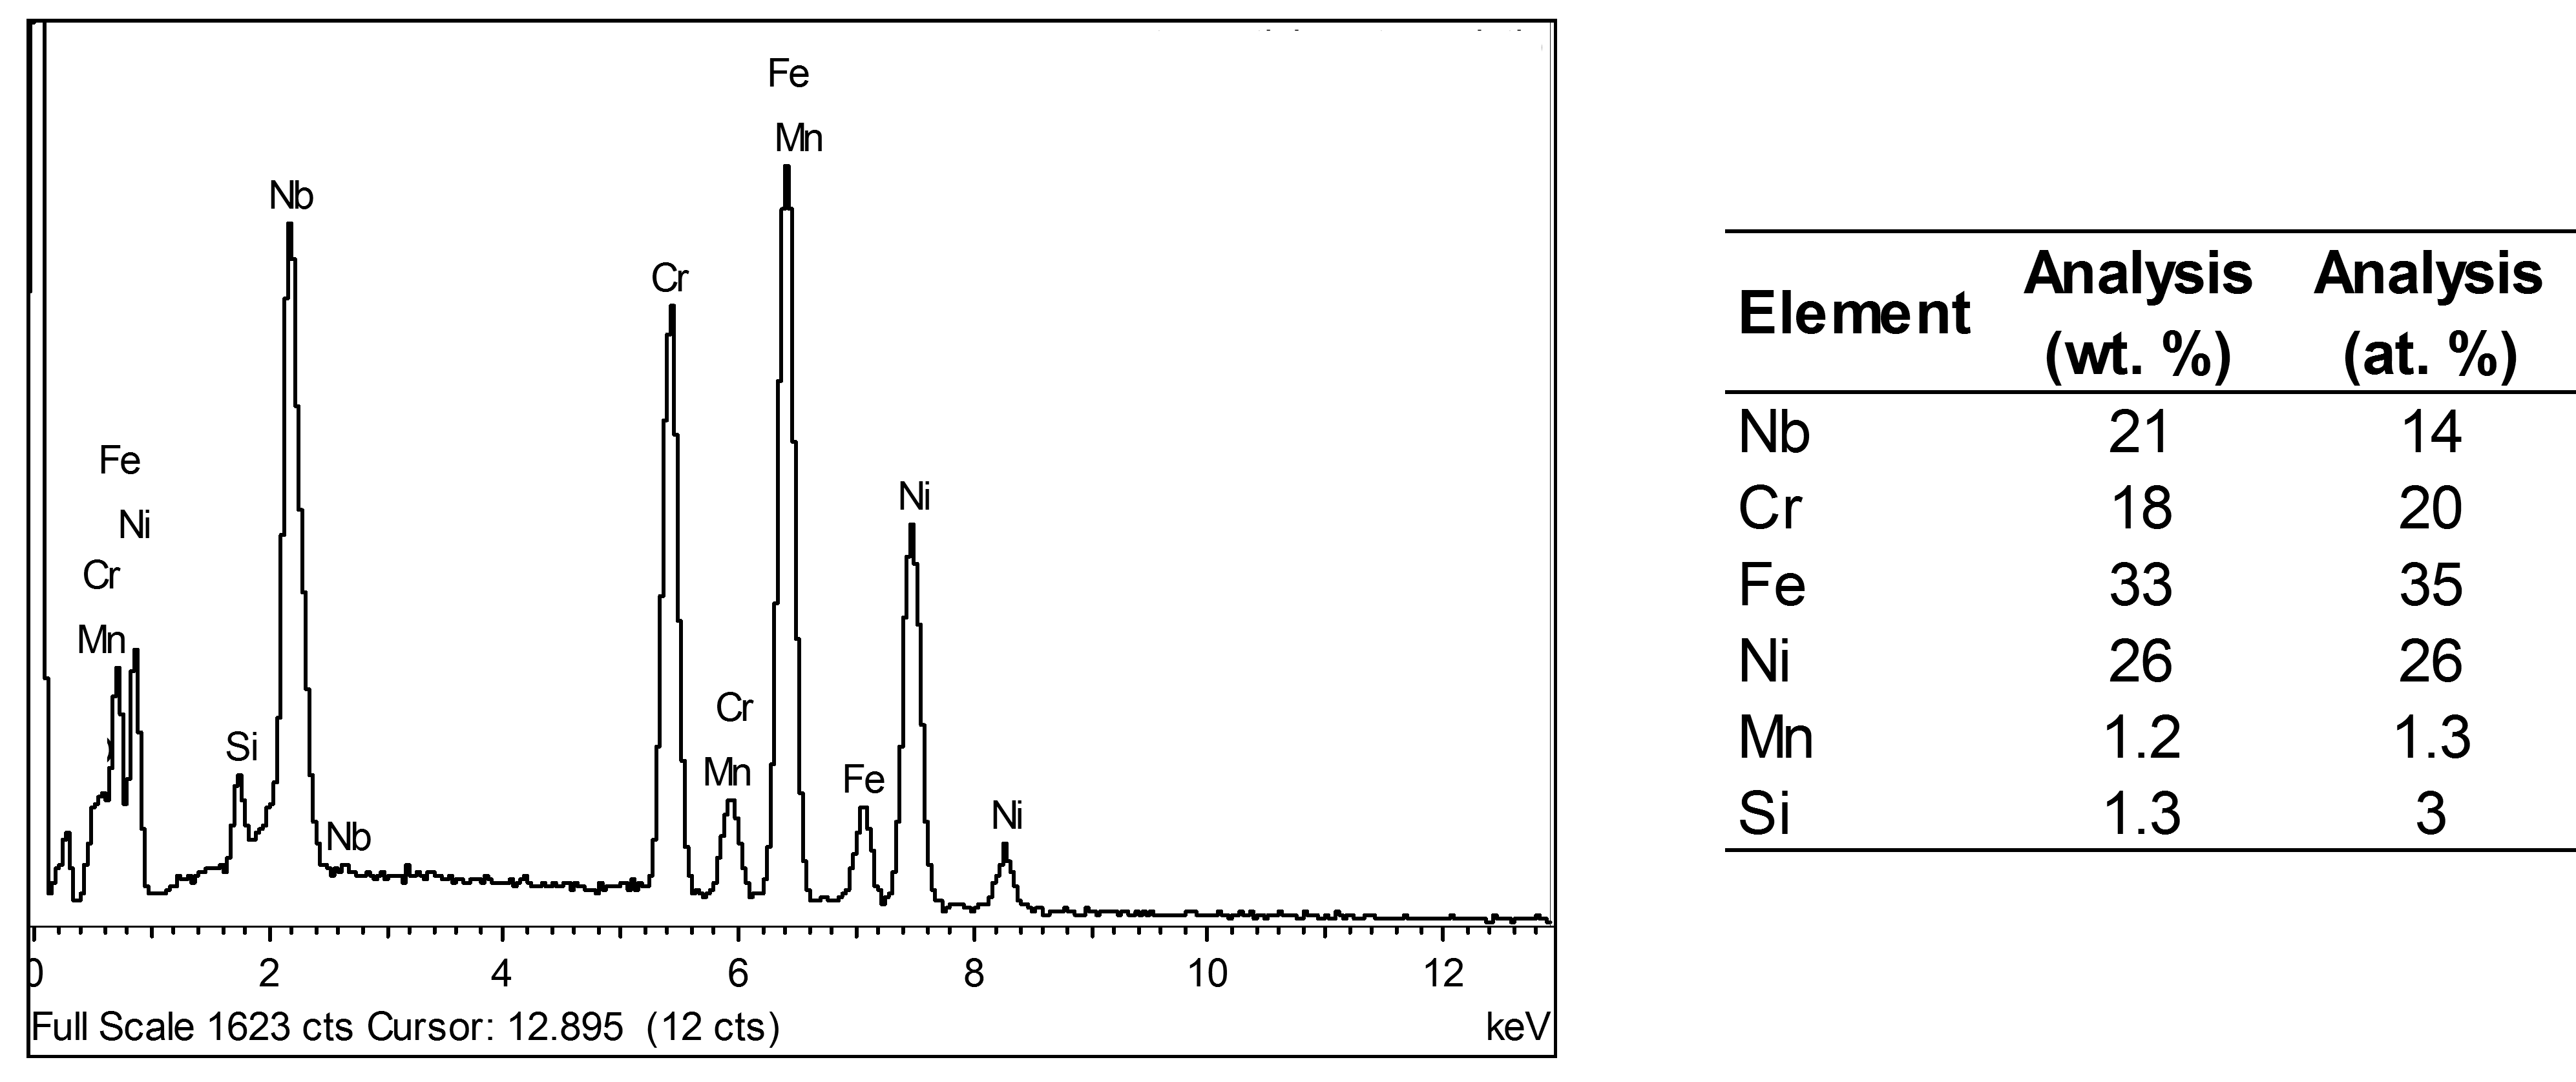
\includegraphics[width=\textwidth]{figures/metallography/c1-oc-2300-crack-tip-particles-eds-table.png}
    \caption{\Gls{eds} results for the boxed area shown in Figure~\ref{subfig:c1-oc-2300-crack-5kx}, at the tip of the crack.}
    \label{fig:c1-oc-2300-crack-tip-particles-eds}
\end{figure}


\begin{figure}
    \centering
    \subfloat[1000X]{\label{subfig:c1-oc-2300-sem-liquid-1kx}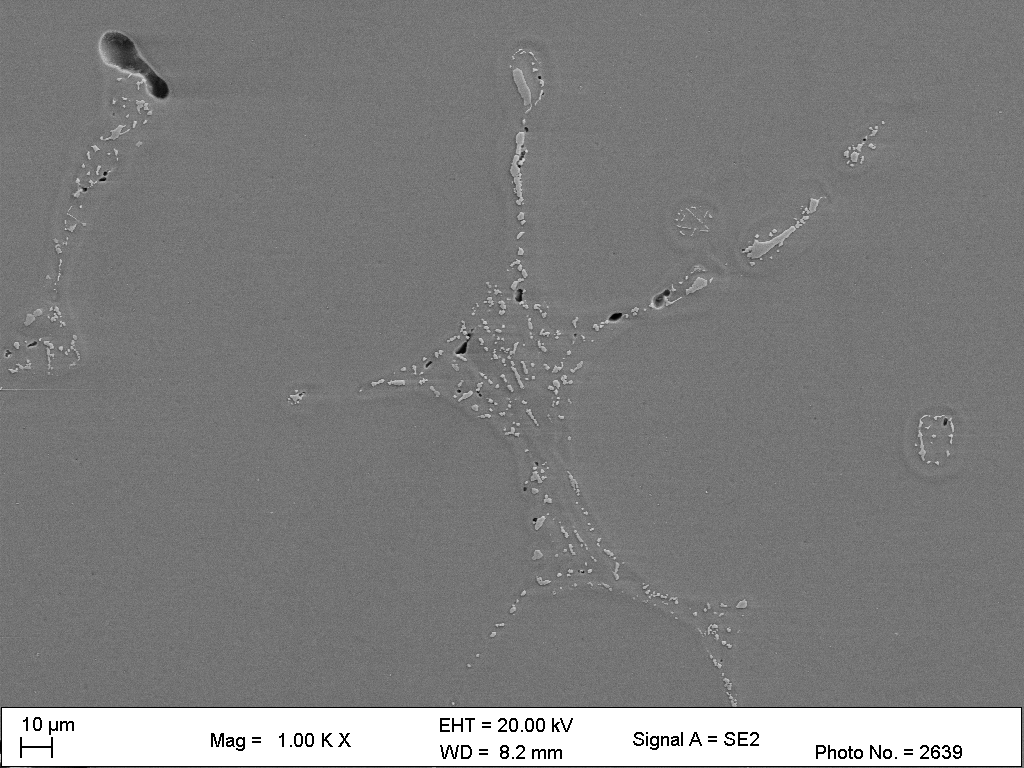
\includegraphics[width=4.7in]{figures/metallography/c1-oc-2300-liquid-L1-1kx-01.png}} \\
    \subfloat[5000X]{\label{subfig:c1-oc-2300-sem-liquid-5kx}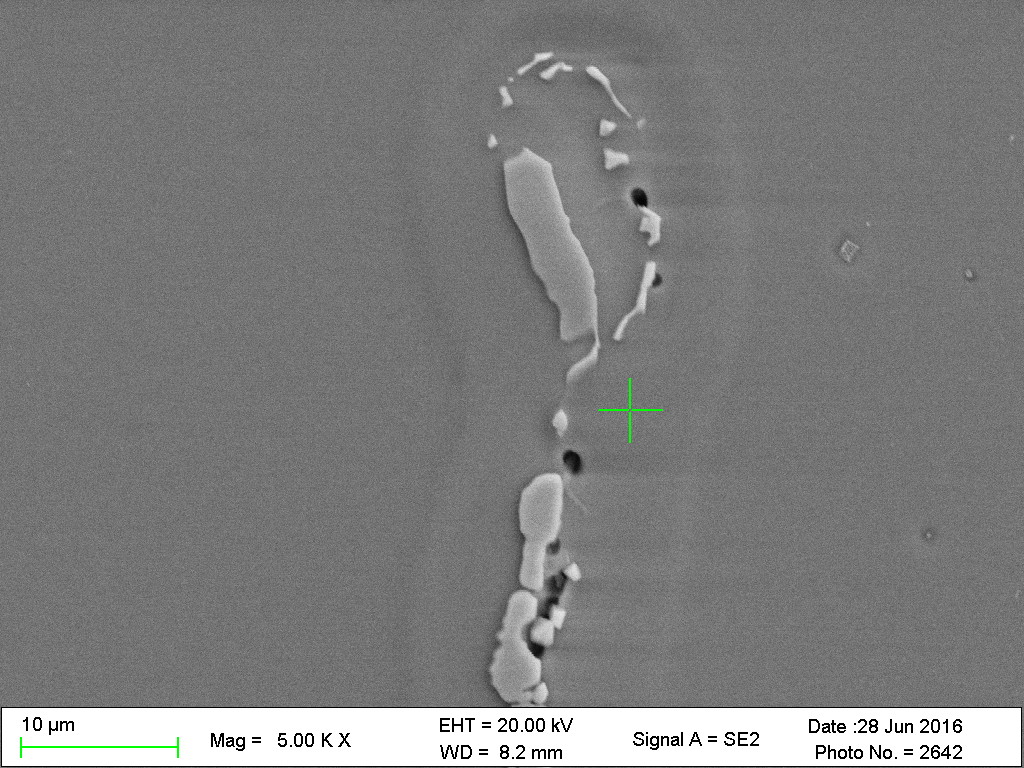
\includegraphics[width=4.7in]{figures/metallography/c1-oc-2300-liquid-L1-5kx-04.png}}
    \caption[]{\Gls{sem} micrographs showing evidence of liquation around interdendritic phases adjacent to the fracture surface in the Cone~1 On-Cooling 2300\textdegree{}F hot ductility sample. \Gls{eds} spot analysis results for the indicated points ``A'' and ``B'' in (b) are given in Figure~\ref{fig:c1-oc-2300-liquid-eds}.}
    \label{fig:c1-oc-2300-sem-liquid}
\end{figure}

\begin{figure}
    \centering
    \subfloat[Spot \gls{eds} results for point ``A'']{\label{subfig:c1-oc-2300-liquid-eds-A}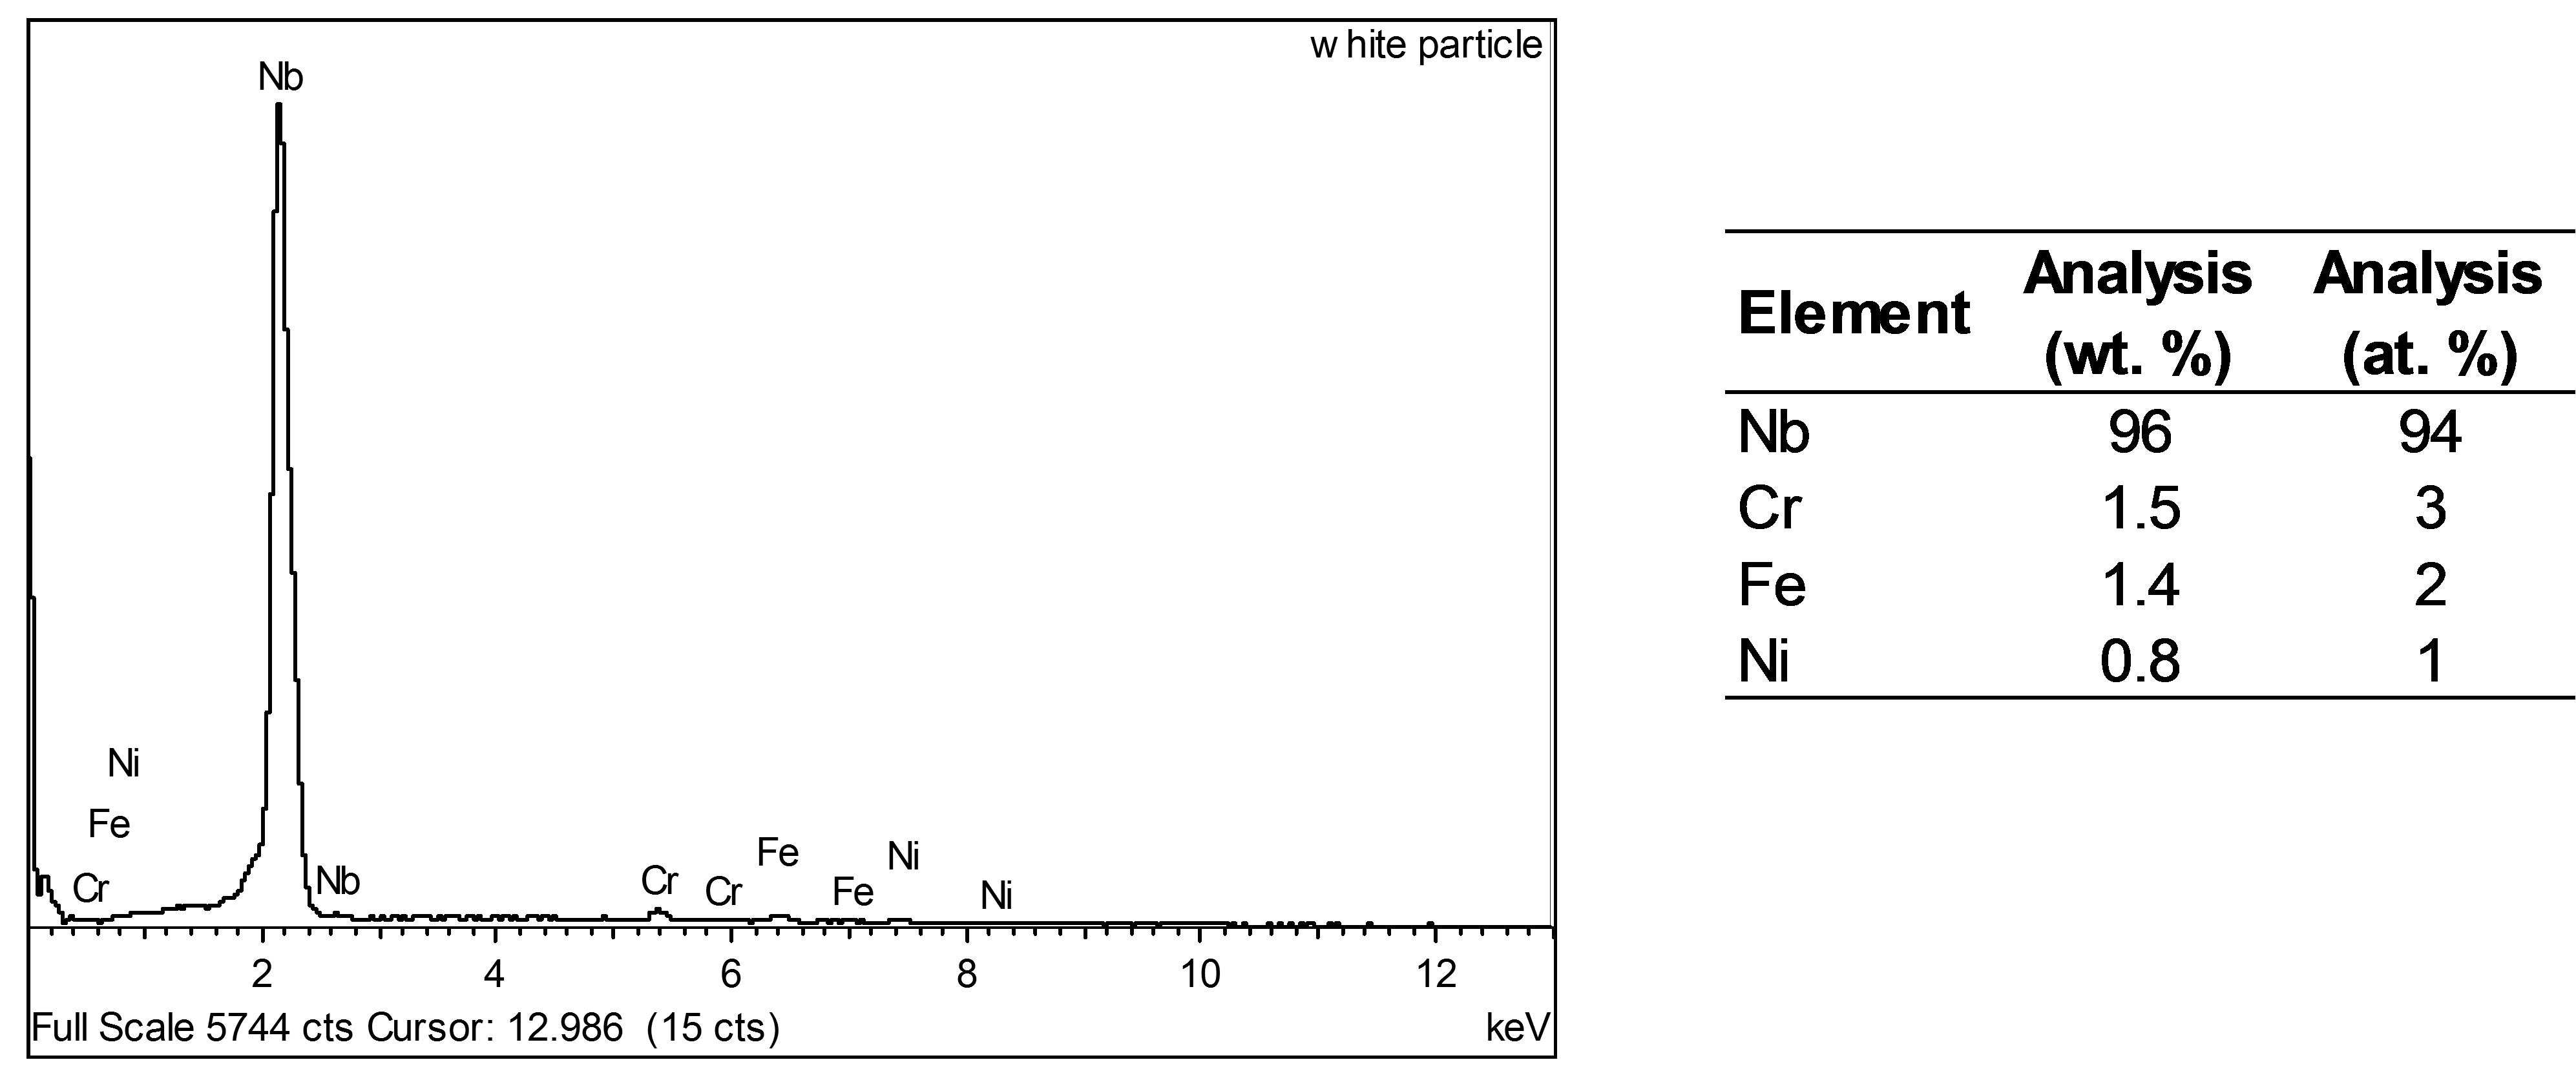
\includegraphics[width=\textwidth]{figures/metallography/c1-oc-2300-liquid-eds-table-A.png}} \\
    \subfloat[Spot \gls{eds} results for point ``B'']{\label{subfig:c1-oc-2300-liquid-eds-B}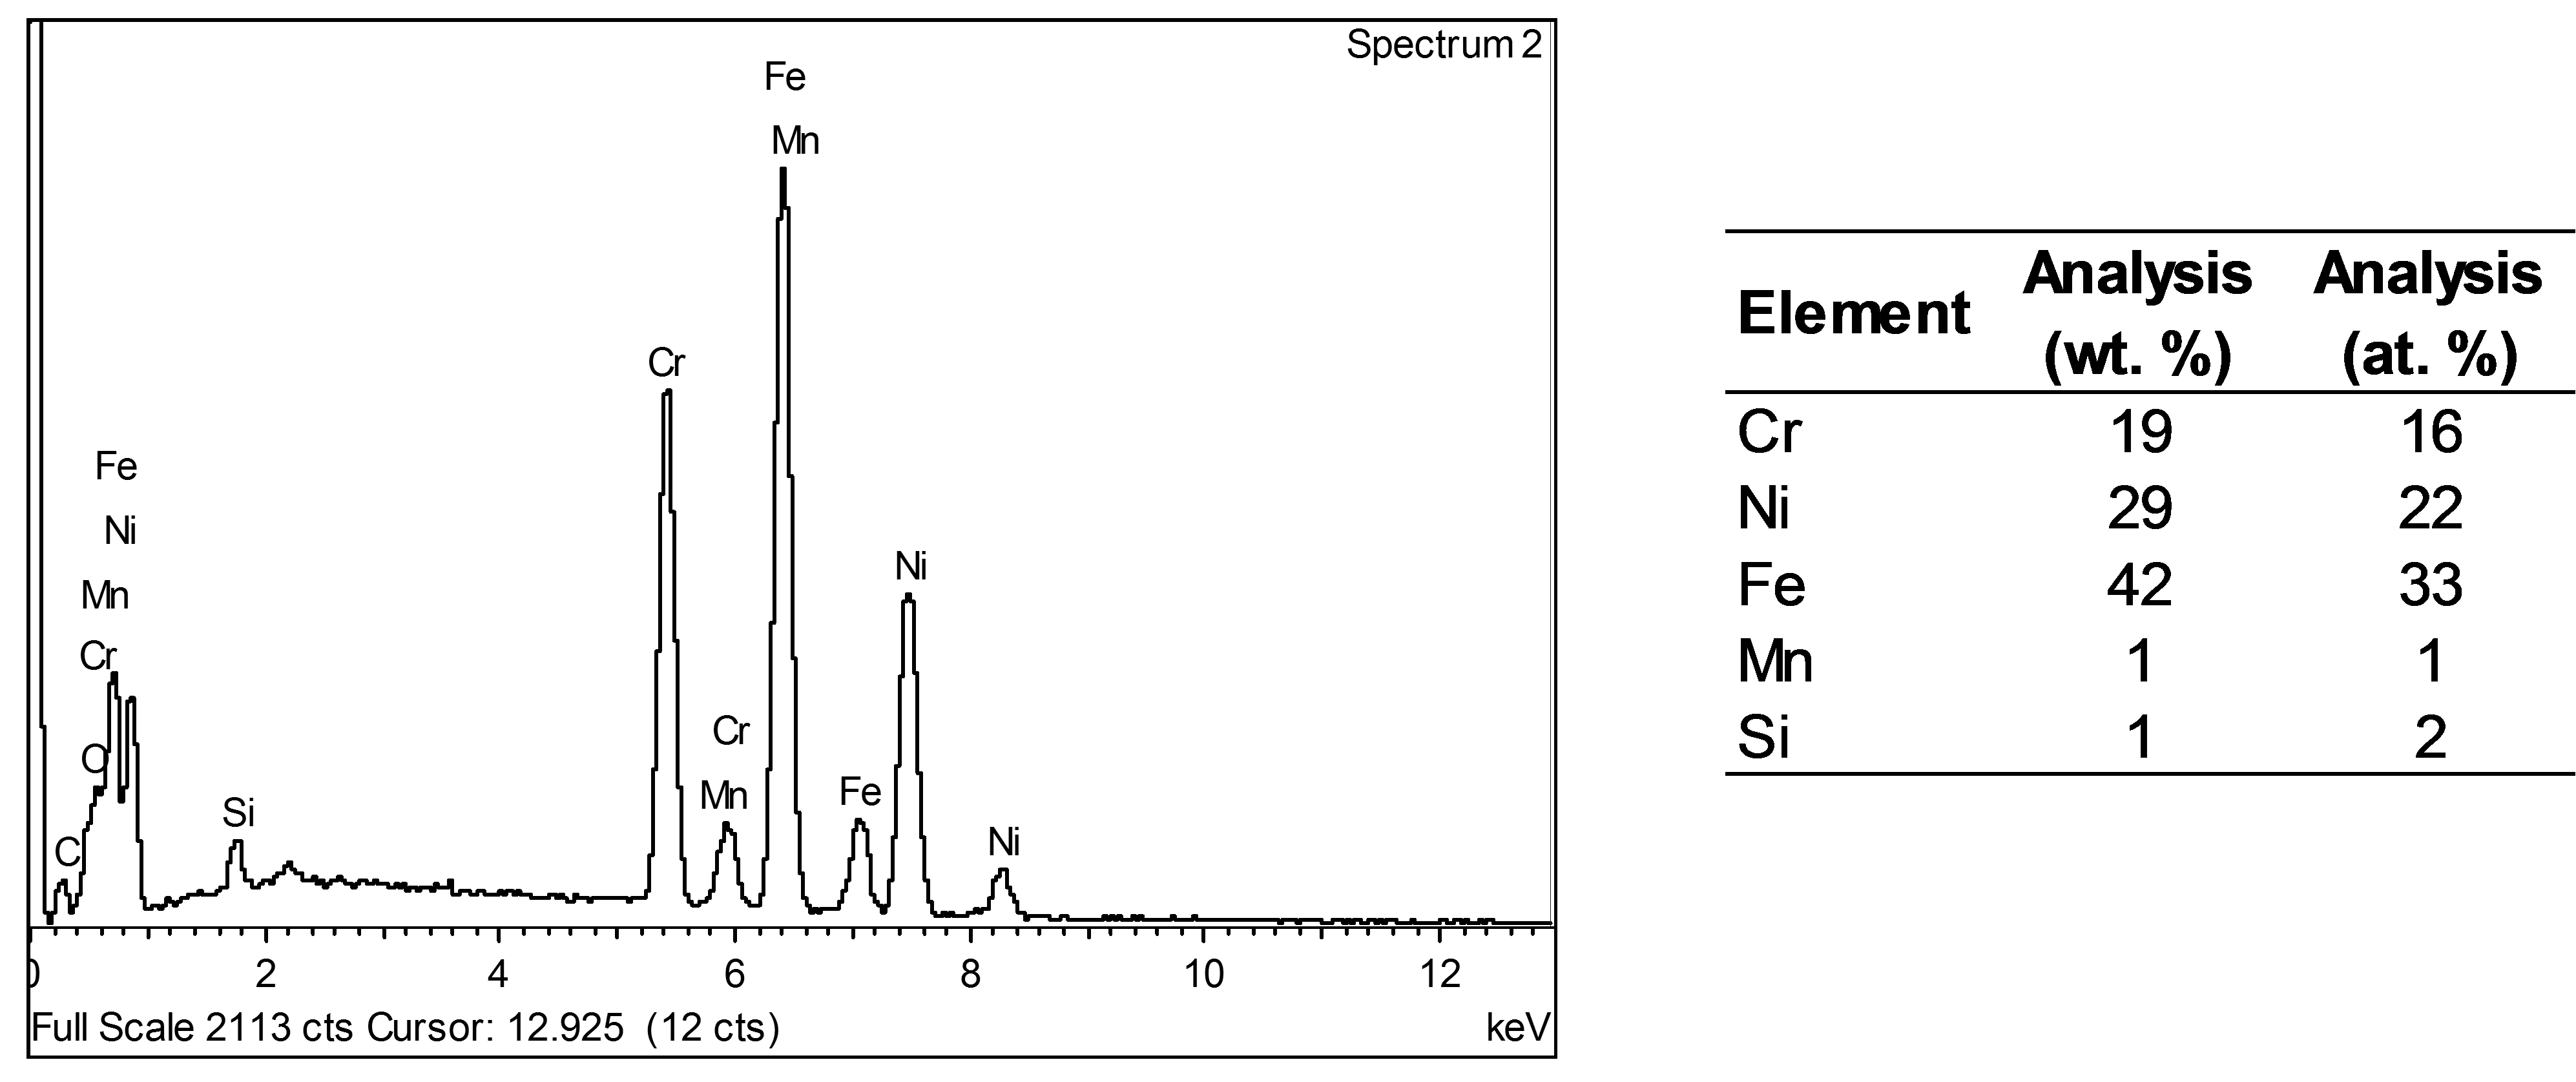
\includegraphics[width=\textwidth]{figures/metallography/c1-oc-2300-liquid-eds-table-B.png}}
    \caption{Spot \gls{eds} results for the indicated points ``A'' and ``B'' in Figure~\ref{subfig:c1-oc-2300-sem-liquid-5kx} for the Cone~1 On-Cooling 2300\textdegree{}F (C1 OC-2300) hot ductility sample.}
    \label{fig:c1-oc-2300-liquid-eds}
\end{figure}
\clearpage

\subsubsection{Cone~5 On-Cooling}
Figure~\ref{fig:c5-oc-2300-fracture-50x} shows a region adjacent to the fracture surface of the Cone~5 On-Cooling 2300\textdegree{}F (C5 OC-2300) hot ductility sample. As with the C1 OC-2300 sample, C5 OC-2300 shows significant cracking along the interdendritic boundaries (with the cracked boundaries generally oriented perpendicular to the tensile loading direction). Extensive liquation is also apparent in Figure~\ref{fig:c5-oc-2300-fracture-50x}, both along the edge of the fracture profile and around the interdendritic phases slightly away from fracture. The extent of prior liquid formed is similar to the C1 OC-2300 sample and as in that case, the greater extent of liquid formation compared to the on-heating test (C5 OH-2375) is due to the longer exposure to the peak temperature of the simulated thermal cycle. The tip of the larger crack, from Figure~\ref{fig:c5-oc-2300-fracture-50x}, is shown at higher magnification in Figure~\ref{fig:c5-oc-2300-crack-olm}, where liquation is evident around the interdendritic boundary ahead of the crack as well as nearby secondary phases (denoted by arrows). The tip of the crack was examined in the \gls{sem} as shown in Figure~\ref{fig:c5-oc-2300-crack-tip-sem}. The compositions of the indicated points in Figure~\ref{subfig:c5-oc-2300-crack-sem-5kx}, corresponding to the liquated region around the crack and a nearby particle, are shown in Figure~\ref{fig:c5-oc-2300-crack-tip-eds} as determined by \gls{eds}. The liquated region near the crack tip shows essentially the nominal alloy composition and does not reveal Ni, Nb, or Si enrichment, while the particle (whitish in appearance) is shown to enriched in Nb (29 wt.\%) and thus most likely a niobium carbide, with other peaks including Cr, Fe, and Ni (with amounts near the nominal alloy composition) in the spectrum from the surrounding matrix.

Another liquated region near the fracture surface is shown in the optical micrographs in Figure~\ref{fig:c5-oc-2300-liquation-olm}. A significant extent of prior liquid formation is evident surrounding a region with a eutectic-like structure. The boxed region in Figure~\ref{subfig:c5-oc-2300-liquation-500x} is examined at higher magnification in the SEM micrographs (using back-scattered electron \gls{bse} imaging mode) presented in Figure~\ref{fig:c5-oc-2300-liquation-sem}. The \gls{eds} results for the three indicated points are given in Figure~\ref{fig:c5-oc-2300-liquation-eds}. Point ``A'' corresponds to the prior liquid and shows a composition close to the nominal alloy composition, but with a slight enrichment in Si and Mn (2.4 wt.\% and 2 wt.\% respectively). It is apparent from Figure~\ref{subfig:c5-oc-2300-crack-sem-5kx} that the phases (highlighted by arrows) at points ``B'' and ``C'' have a different appearance from the surrounding brighter ``white''-appearing particles (which are NbC), resulting from the chemical composition contrast provided by \gls{bse} imaging. Both phases analyzed at points ``B'' and ``C'' are enriched in Si, Ni, and Nb compared to the nominal alloy composition. However, the \gls{eds} compositions are not close to that of G-phase (Ni16Nb6Si7) which has a composition of 55.8 wt.\% Ni, 32.9 wt.\% Nb, and 11.6 wt.\% Si \cite{hoffman_high_2000-1}. Furthermore, these phases were present only to an extremely minimal extent in the C5 OC-2300 sample and were isolated in distribution, indicating that these Ni-Nb-Si enriched phases (which do not appear to correlate with G-phase) could not significantly contribute to the observed liquation along the interdendritic boundaries. Considering the observed eutectic-like structures containing NbC in conjunction with solidified liquid (e.g. Figure~\ref{fig:c5-oc-2300-liquation-olm}), it is possible that a constitutional liquation reaction between NbC and austenite is responsible for the observed liquation along the interdendritic boundaries with subsequent formation of a NbC-austenite eutectic upon resolidification. \citet{lee_weldability_1988} investigated the hot ductility behavior of 347NG (nuclear grade) stainless steel, which is niobium stabilized and contains NbC carbides, and observed NbC-austenite eutectic constituents associated with constitutional liquation along grain boundaries.

%Ni-Nb-Si enriched phases were found only rarely, and the liquid observed in both on-heating and on-cooling tests was not found to be enriched in these elements

% Patchett suggested that the liquation cracking mechanism follows a Thompson constitutional liquation model with NbC and a Si-Ni phase

\begin{figure}
    \centering
    \includegraphics[width=4.7in]{figures/metallography/c5-oc-2300-fracture-50x.png}
    \caption{Optical micrograph showing a region adjacent to the fracture surface in the Cone~5 On-Cooling 2300\textdegree{}F (C5 OC-2300) hot ductility sample. Etch: electrolytic 10\% oxalic acid.}
    \label{fig:c5-oc-2300-fracture-50x}
\end{figure}

\begin{figure}
    \centering
    \subfloat[100X]{\label{subfig:c5-oc-2300-crack-100x}\includegraphics[width=4.7in]{figures/metallography/c5-oc-2300-crack-100x.png}} \\
    \subfloat[500X]{\label{subfig:c5-oc-2300-crack-500x}\includegraphics[width=4.7in]{figures/metallography/c5-oc-2300-crack-tip-500x.png}}
    \caption{Optical micrographs showing the crack visible in Figure~\ref{fig:c5-oc-2300-fracture-50x} for the Cone~5 On-Cooling 2300\textdegree{}F (C5 OC-2300) hot ductility sample. Liquated regions around the crack tip and interdendritic phases are denoted by arrows. Etch: electrolytic 10\% oxalic acid.}
    \label{fig:c5-oc-2300-crack-olm}
\end{figure}

\begin{figure}
    \centering
    \subfloat[1000X]{\label{subfig:c5-oc-2300-crack-sem-1kx}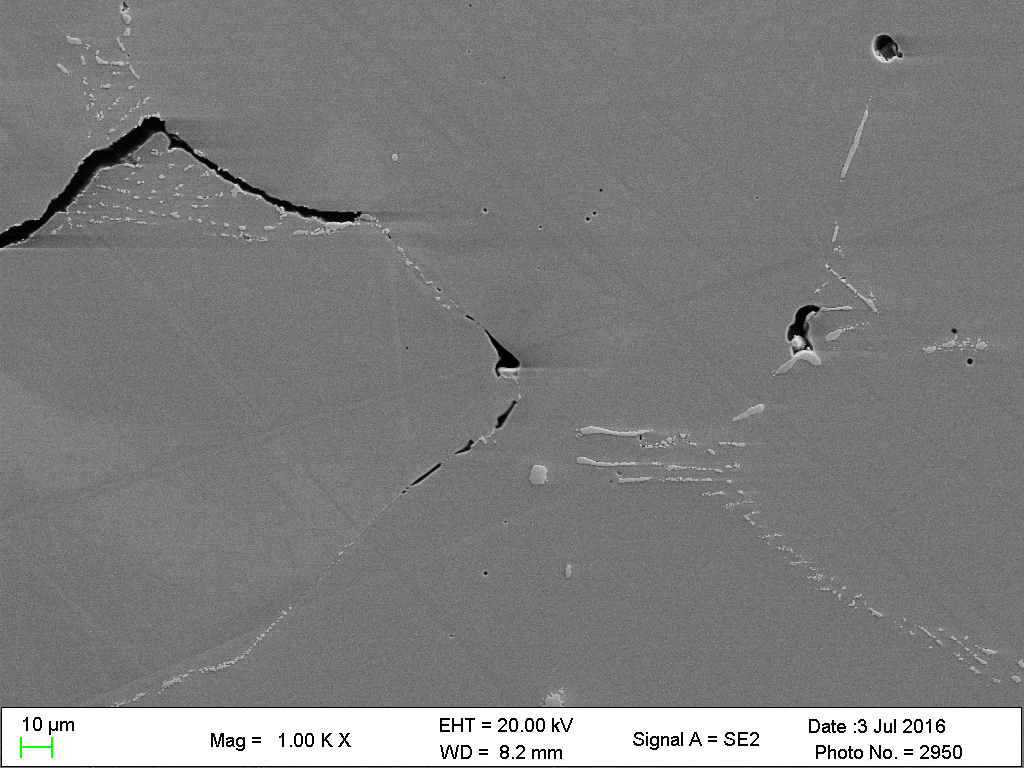
\includegraphics[width=4.7in]{figures/metallography/c5-oc-2300-crack-sem-1kx-L2-21.png}} \\
    \subfloat[5000X]{\label{subfig:c5-oc-2300-crack-sem-5kx}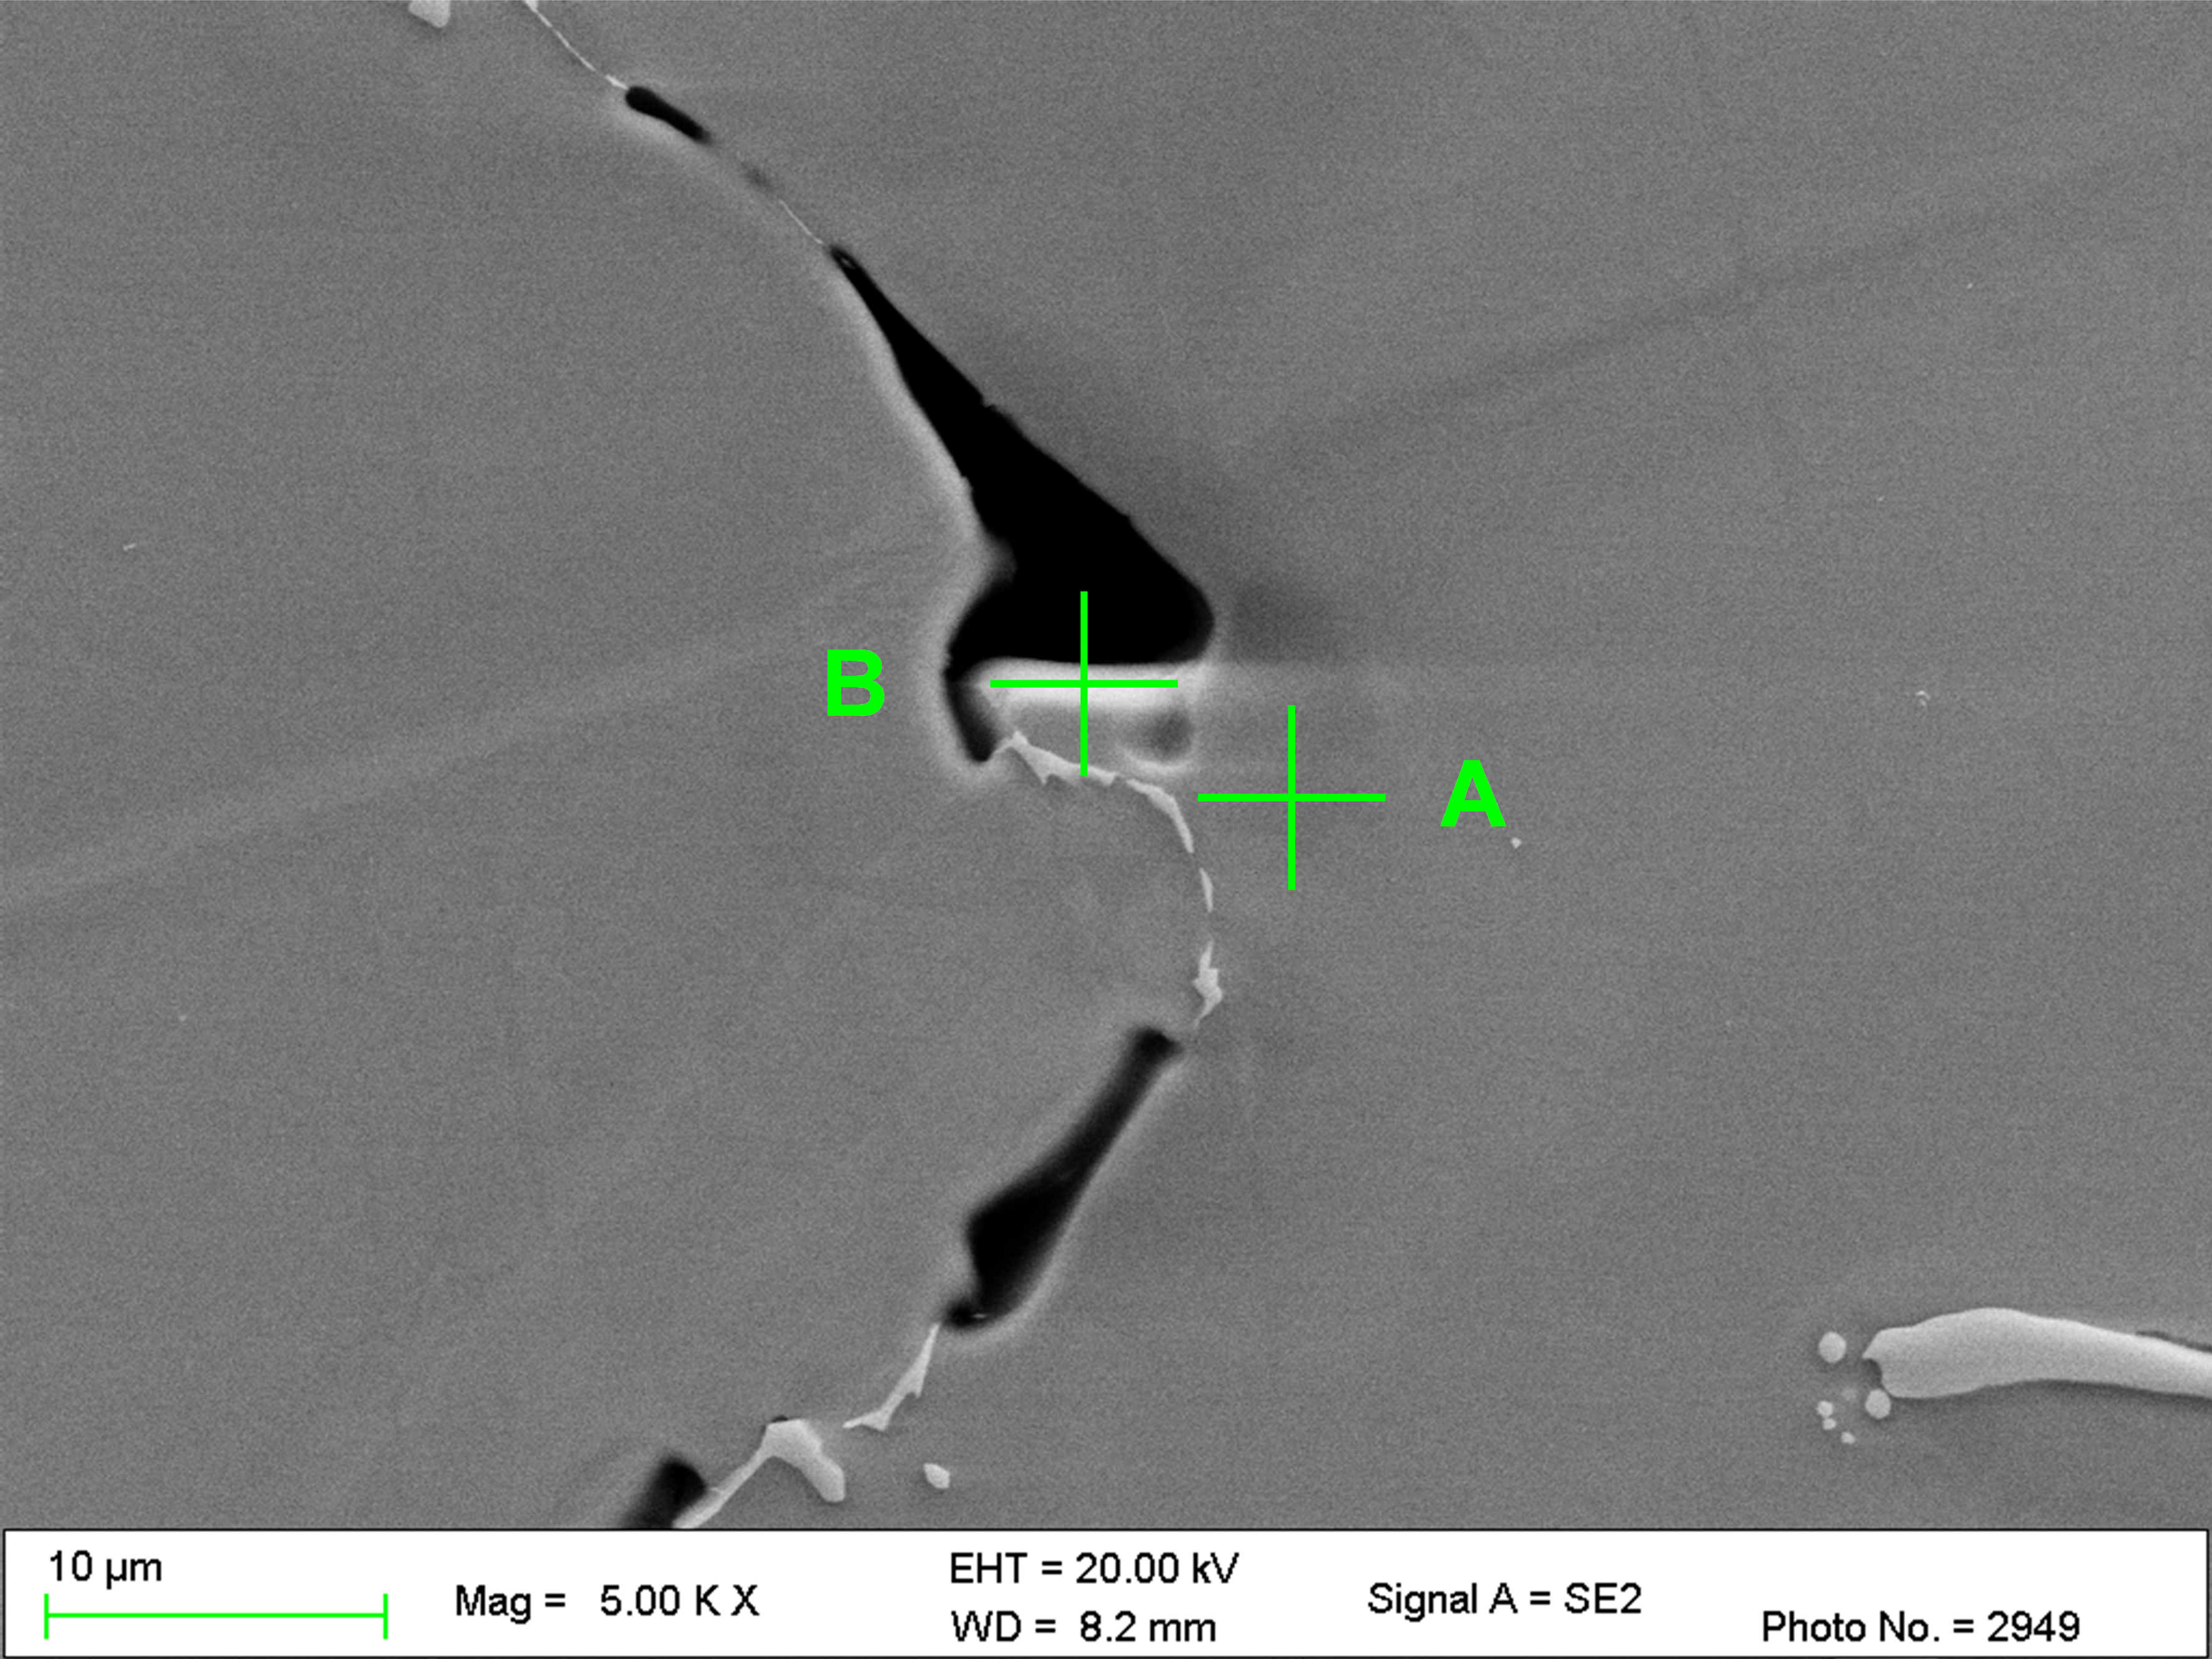
\includegraphics[width=4.7in]{figures/metallography/c5-oc-2300-crack-sem-5kx-L2-20.png}}
    \caption{\Gls{sem} micrographs of a crack tip region (cf. Figure~\ref{fig:c5-oc-2300-crack-olm}) in the Cone~5 On-Cooling 2300\textdegree{}F (C5 OC-2300) hot ductility sample. The \gls{eds} results for the indicated points ``A'' and ``B'' are given in Figure~\ref{fig:c5-oc-2300-crack-tip-eds}. Etch: electrolytic 10\% oxalic acid.}
    \label{fig:c5-oc-2300-crack-tip-sem}
\end{figure}

\begin{figure}
    \centering
    \subfloat[Spot \Gls{eds} results for point ``A'']{\label{subfig:c5-oc-2300-crack-eds-A}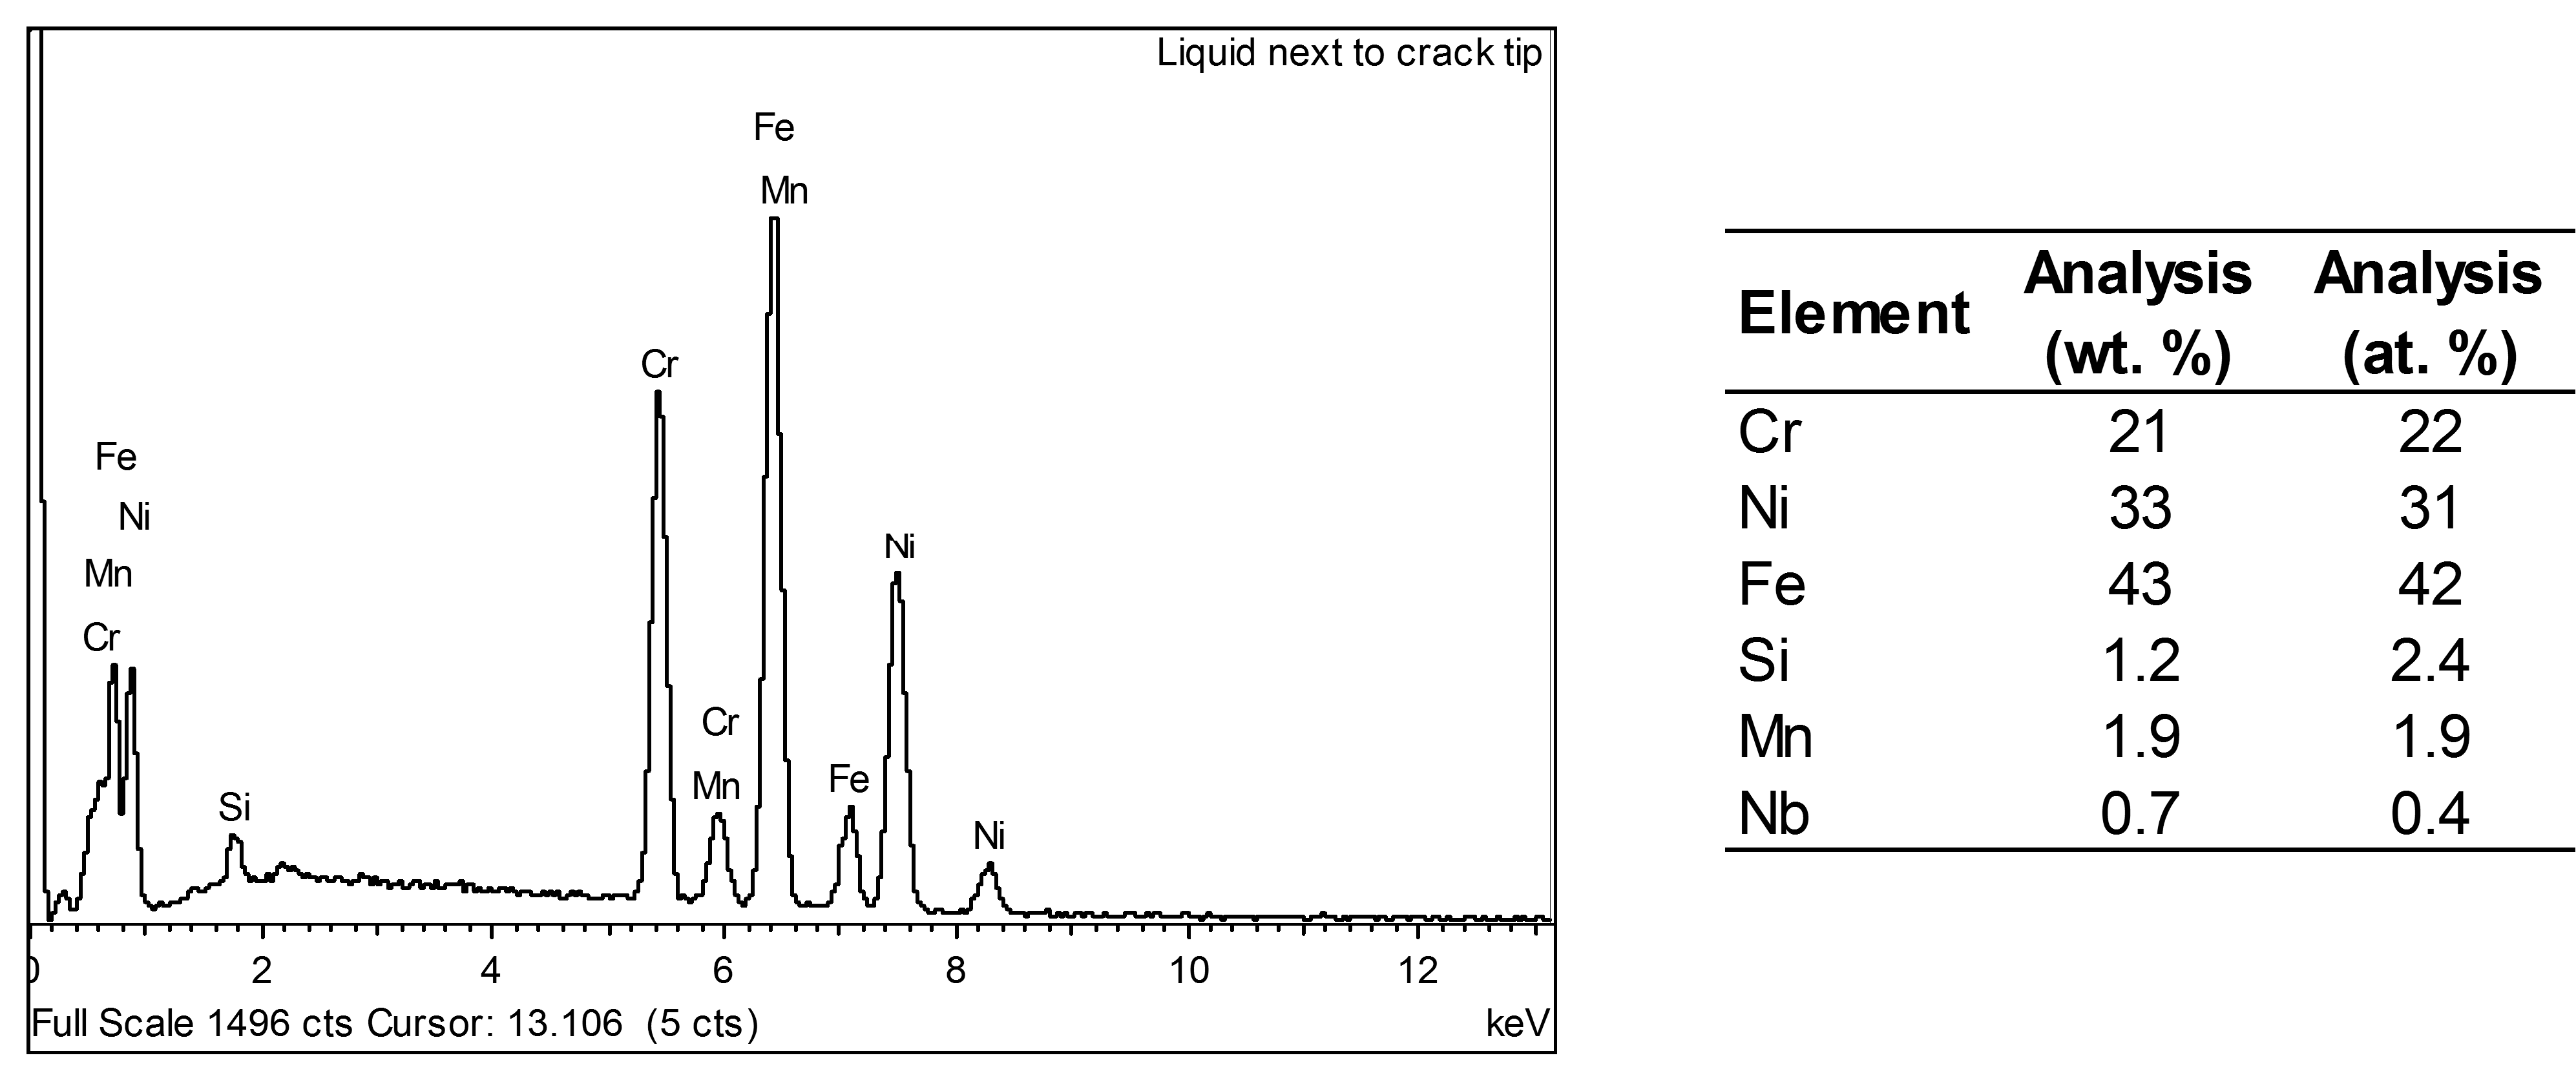
\includegraphics[width=\textwidth]{figures/metallography/c5-oc-2300-crack-eds-table-A.png}} \\
    \subfloat[Spot \Gls{eds} results for point ``B'']{\label{subfig:c5-oc-2300-crack-eds-B}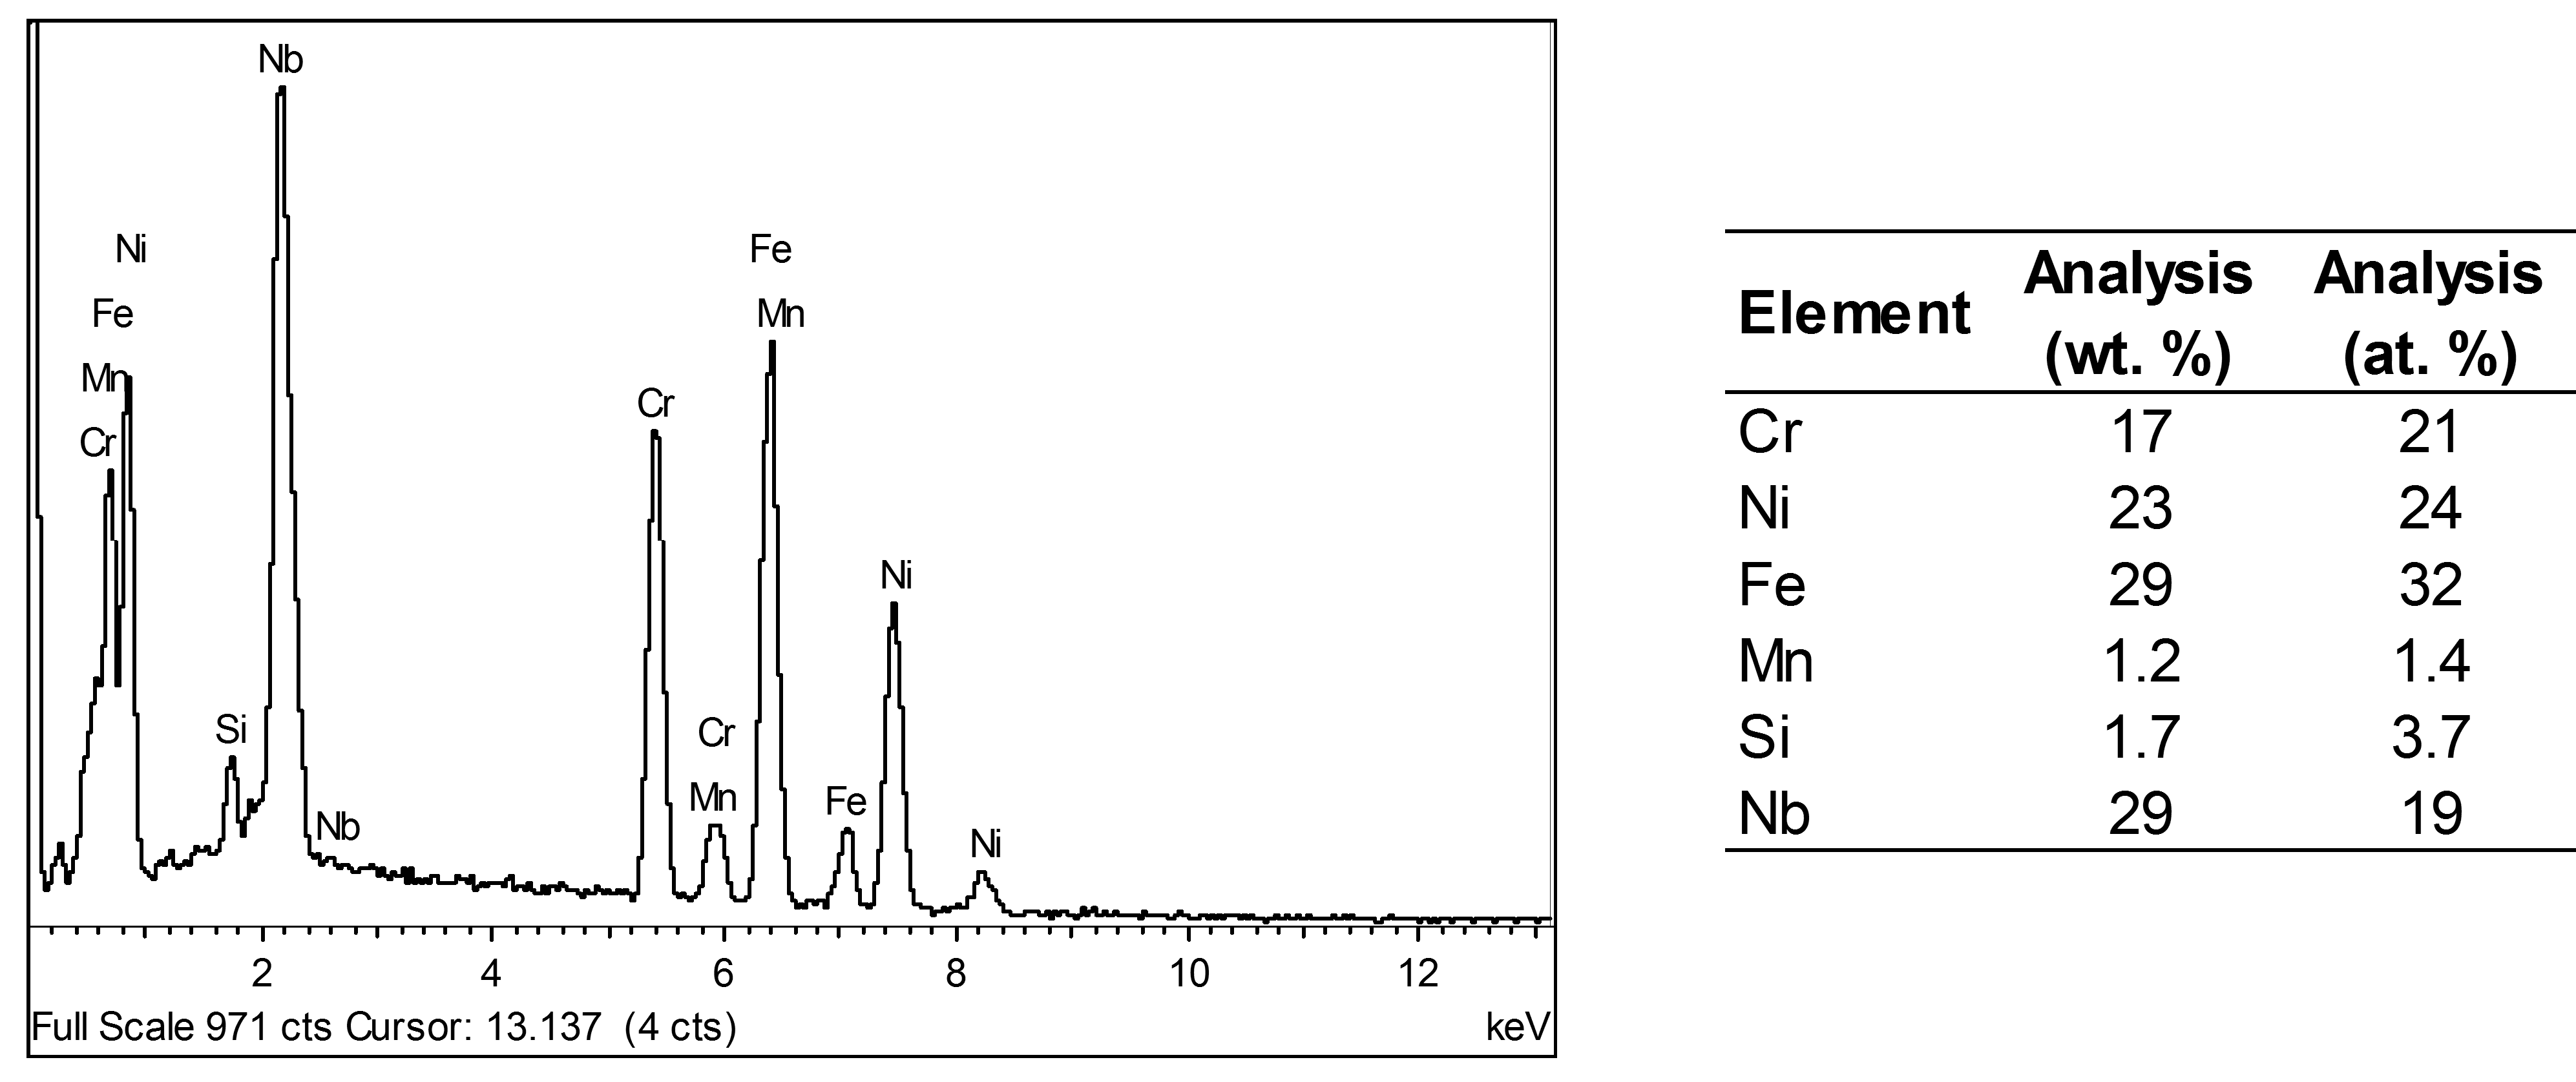
\includegraphics[width=\textwidth]{figures/metallography/c5-oc-2300-crack-eds-table-B.png}}
    \caption{Spot \gls{eds} results for indicated points ``A'' and ``B'' in Figure~\ref{fig:c5-oc-2300-crack-tip-sem} at a crack tip region in the Cone~5 On-Cooling 2300\textdegree{}F (C5 OC-2300) hot ductility sample.}
    \label{fig:c5-oc-2300-crack-tip-eds}
\end{figure}


\begin{figure}
    \centering
    \subfloat[100X]{\label{subfig:c5-oc-2300-liquation-100x}\includegraphics[width=4.7in]{figures/metallography/c5-oc-2300-liquation-100x.png}} \\
    \subfloat[500X]{\label{subfig:c5-oc-2300-liquation-500x}\includegraphics[width=4.7in]{figures/metallography/c5-oc-2300-liquation-500x.png}}
    \caption{Optical micrographs showing a liquated region adjacent to the fracture surface in the Cone~5 On-Cooling 2300\textdegree{}F (C5 OC-2300) hot ductility sample. The boxed region in (b) is examined at higher magnification in Figure~\ref{fig:c5-oc-2300-liquation-sem}. Etch: electrolytic 10\% oxalic acid.}
    \label{fig:c5-oc-2300-liquation-olm}
\end{figure}

\begin{figure}
    \centering
    \subfloat[2500X]{\label{subfig:c5-oc-2300-liquation-sem-2-5kx}\includegraphics[width=4.7in]{figures/metallography/c5-oc-2300-liquation-sem-2-5kx-L4-46.png}} \\
    \subfloat[5000X]{\label{subfig:c5-oc-2300-liquation-sem-5kx}\includegraphics[width=4.7in]{figures/metallography/c5-oc-2300-liquation-sem-5kx-L4-37.png}}
    \caption{\glsentryshort{bse}-\gls{sem} micrographs of the boxed region from Figure~\ref{fig:c5-oc-2300-liquation-olm} showing liquation surrounding interdendritic phases in the Cone~5 On-Cooling 2300\textdegree{}F (C5 OC-2300) hot ductility sample. \gls{eds} results for the three indicated points in (b) are given in Figure~\ref{fig:c5-oc-2300-liquation-eds}. Etch: electrolytic 10\% oxalic acid.}
    \label{fig:c5-oc-2300-liquation-sem}
\end{figure}

\begin{figure}
    \centering
    \subfloat[Spot \Glsentryshort{eds} results for point ``A'' corresponding to prior liquid in Figure~\ref{subfig:c5-oc-2300-liquation-sem-5kx}]{\label{subfig:c5-oc-2300-liquation-eds-table-A}\includegraphics[width=5.5in]{figures/metallography/c5-oc-2300-liquation-eds-table-A.png}} \\
    \subfloat[Spot \Gls{eds} results for point ``B'']{\label{subfig:c5-oc-2300-liquation-eds-table-B}\includegraphics[width=5.5in]{figures/metallography/c5-oc-2300-liquation-eds-table-B.png}} \\
    \subfloat[Spot \Gls{eds} results for point ``C'']{\label{subfig:c5-oc-2300-liquation-eds-table-C}\includegraphics[width=5.5in]{figures/metallography/c5-oc-2300-liquation-eds-table-C.png}}
    \caption{Spot \gls{eds} results for indicated points ``A'', ``B'', and ``C'' in Figure~\ref{fig:c5-oc-2300-liquation-sem} at a liquated region in the Cone~5 On-Cooling 2300\textdegree{}F (C5 OC-2300) hot ductility sample.}
    \label{fig:c5-oc-2300-liquation-eds}
\end{figure}
    %!TEX root = ..\ms-thesis.tex
\chapter{Conclusions} \label{ch:conclusions}
Two centrifugally-cast, 20Cr-32Ni-1Nb hydrogen reformer outlet manifold components were evaluated using the Gleeble\texttrademark{} hot ductility test to determine the potential susceptibility to \gls{haz} liquation cracking.  The evaluation revealed the following:

\begin{enumerate}
\item Both 20Cr-32Ni-1Nb heats (Cone~1 and Cone~5) exhibited similar as-received microstructures, with numerous NbC carbides along the interdendritic boundaries. A significant extent of fine intradendritic precipitates was also observed in the as-received material. However, evidence of Ni-Nb-Si enriched phases adjoining the interdendritic NbC, commonly reported for service-exposed (“aged”) 20Cr-32Ni-1Nb material, was not observed. Thus, it is likely that both materials in the current study were subjected to a solution-annealing treatment after removal from service, contrary to the stated condition.
\item Both Cone~1 and Cone~5 exhibited Class H1 hot ductility behavior when tested on-heating, with an on-heating \gls{zdt} of 2375\textdegree{}F. Class H1 on-heating behavior is not, in and of itself, indicative of high sensitivity to liquation cracking.
\item Based on the Nippes criteria, both Cone materials exhibited Class C3 behavior when tested upon cooling from peak temperatures equal to the \gls{zdt}.  Class C3 behavior corresponds to a generally poor recovery of on-cooling ductility after exposure to the \gls{haz} peak temperature.  This classification of the Cone 1 and Cone 5 on-cooling behavior was further corroborated by observed \gls{zdr}s of 75 F\textdegree{} and calculated DRR values on the order of 20\% at 2225\textdegree{}F for both Cone materials.
\item On the basis of the observed Class-H1/Class-C3 behavior together with the determined values of the \gls{zdr} and \gls{drr} criteria, the Cone 1 and Cone 5 materials were shown to be sensitive to liquation cracking in the base metal HAZ. Furthermore, considering the possibility that the Cone~1 and Cone~5 materials were in the solution-annealed condition, the liquation cracking susceptibility of service-exposed material is expected to be on a similar or, more likely, higher level. In any case, hot ductility testing during the early stages of development of the 20Cr-32Ni-1Nb alloy would have revealed the susceptibility to liquation cracking and this information would have been valuable for avoiding the repair welding problems experienced by industry.
\item The Cone~1 and Cone~5 hot ductility samples tested on-heating at 2375\textdegree{}F showed similar microstructures exhibiting cracking along the interdendritic boundaries decorated with NbC and dissolution of fine intradendritic precipitates near the fracture surface. At this test temperature, corresponding to the \gls{zdt}, the beginning of liquation at some interdendritic boundaries was apparent, and this liquation was the cause of the observed nil ductility behavior at this temperature.
\item In the Cone~1 and Cone~5 hot ductility samples tested on-cooling at 2300\textdegree{}F after exposure to the \gls{zdt}, cracking along the interdendritic boundaries near the fracture surface was again observed accompanied by dissolution of fine intradendritic precipitates. Compared to the on-heating tests, a significantly greater extent of liquation around crack faces and interdendritic phases was apparent, due to longer exposure time near the peak temperature of the simulated thermal cycle (longer time near the \gls{zdt}). The extensive liquation was responsible for the observed nil ductility behavior at the \gls{drt}.
\item In all of the on-heating and on-cooling hot ductility samples, the composition of the prior liquid present at liquated boundaries was not significantly different from the nominal alloy composition and in particular did not show evidence of Ni, Nb, or Si enrichment that would suggest that incipient melting of Ni-Nb-Si enriched phases (G-phase) was responsible for the observed liquation.
\item Due to the essential absence of Ni-Nb-Si enriched phases in both the as-received materials and tested hot ductility samples, the observed liquation of interdendritic boundaries at temperatures below the bulk solidus temperature was attributed to constitutional liquation of NbC located on the boundaries.

\end{enumerate}

%{\item The fracture paths in a Cone 5 On-Heating 2375\textdegree{}F (ZDT) sample were observed to proceed along the interdendritic boundaries, and the crack faces were closely associated with the interdendritic secondary phases. }

%and would thus warrant appropriate precautions during welding to prevent the occurrence of cracking

    %!TEX root = ..\ms-thesis.tex
\chapter{Future Work} \label{ch:future-work}
\begin{enumerate}
\item Having characterized the hot ductility behavior of 20Cr-32Ni-Nb material which was known to be crack-sensitive (the current work) and thereby established a basis for comparison, the hot ductility behavior of modified chemistry heats of 20Cr-32Ni-Nb should be investigated, for example the modified chemistry suggested by (Hoffman chemistry modifications) which [changes to chemistry]. These modified chemistry materials showed improved mechanical properties after service exposure compared to the typical chemistry and thus the modified chemistry appears promising in terms of reducing the liquation cracking propensity of the alloy.
\item Because it has been observed that cast tee and cast cone materials exhibit different reductions in mechanical properties after service exposure, hot ductility evaluation of cast tee materials should be performed to quantify the cracking propensity of statically cast materials (with potentially larger grain size and greater formation of secondary phases) using criteria that are directly related to welding (rather than more general methods such as tensile testing).
\item Dissolution of bulk samples from as-service exposed and simulated HAZ samples to extract precipitates for XRD analysis to quantitatively evaluate the phase fractions and changes thereof during welding
\item Evaluation of carbon extraction replicas in TEM for quantitative composition of secondary phases using EDXS or electron diffraction
\item TTP data for standard and modified CT15C chemistries to determine over what temperatures the silicide phase forms, is stable, etc... and to see if the modified chemistry shows improved behavior in the long term (\emph{did Hoffman show that modified chemistry resulted in lesser extent of G-phase??})
\end{enumerate}

    %%%%%%%%%%%%%%%%%%%%%%%%%%%%%%%%%%%%%%%%%%%%%%%%%%%%%%%%%%%%%%%%%%%%%%%%%%%%%%%%%%%%%%%%%%%%%%%%%%%%%
    % BIBLIOGRAPHY
    %%%%%%%%%%%%%%%%%%%%%%%%%%%%%%%%%%%%%%%%%%%%%%%%%%%%%%%%%%%%%%%%%%%%%%%%%%%%%%%%%%%%%%%%%%%%%%%%%%%%%
    \makeBibliographyPage % make the bibliography title page - can be edited in ut-thesis-template.tex
    %\bibliographystyle{ieeetran} % bibliography style - recommend using apalike-doi as it hyperlinks DOIs
    %\bibliography{references/references-thesis} % references.bib included in the references directory
    \printbibliography
    %%%%%%%%%%%%%%%%%%%%%%%%%%%%%%%%%%%%%%%%%%%%%%%%%%%%%%%%%%%%%%%%%%%%%%%%%%%%%%%%%%%%%%%%%%%%%%%%%%%%%
    % APPENDIX - OPTIONAL - COMMENT IF NOT NEEDED
    %%%%%%%%%%%%%%%%%%%%%%%%%%%%%%%%%%%%%%%%%%%%%%%%%%%%%%%%%%%%%%%%%%%%%%%%%%%%%%%%%%%%%%%%%%%%%%%%%%%%%
    \makeAppendixPage   % make the appendix title page - can be edited in ut-thesis-template.tex
    \appendix
    \chapter{Summary of Equations}
\section{Cartesian}
some equations here

\section{Cylindrical}
some equations also here
    %%%%%%%%%%%%%%%%%%%%%%%%%%%%%%%%%%%%%%%%%%%%%%%%%%%%%%%%%%%%%%%%%%%%%%%%%%%%%%%%%%%%%%%%%%%%%%%%%%%%%
    % A VITA IS REQUIRED
    %%%%%%%%%%%%%%%%%%%%%%%%%%%%%%%%%%%%%%%%%%%%%%%%%%%%%%%%%%%%%%%%%%%%%%%%%%%%%%%%%%%%%%%%%%%%%%%%%%%%%
    \addToTOC{Vita}
    \chapter*{Vita} \label{ch:vita}
John Bohling was born in Visalia, CA to his parents, Mark and Sandra Bohling. He is the oldest of four sons. After a cross-country move with his family, John attended Auburn High School in Auburn, AL, and graduated in 2005. After working for a year, he enrolled at the University of Tennessee, Knoxville in the fall of 2006. He graduated with a Bachelor of Science in Materials Science and Engineering in December 2010. During his undergraduate studies, his classes on metallurgy and welding sparked his interest in these areas, and the following year, he started his graduate studies at the University of Tennessee with Dr. Carl Lundin in the area of materials joining and welding metallurgy. John graduated with his Master of Science in Materials Science and Engineering, with a concentration in metallurgy, in August 2016. He is continuing his graduate work with Dr. Lundin at the University of Tennessee for a Ph.D. in Materials Science and Engineering.
\end{document}
